\documentclass[12pt,a4paper]{article}
%% Generated by scripts/build_report.py from report/src/report.md - edit the source, not this file.
%% Compile on Overleaf with pdfLaTeX; BibTeX runs automatically.
\usepackage[T1]{fontenc}
\usepackage[utf8]{inputenc}
%% fallbacks so a stray Unicode dash or space cannot stop the compile (and leave citations undefined)
\DeclareUnicodeCharacter{2010}{-}
\DeclareUnicodeCharacter{2011}{-}
\DeclareUnicodeCharacter{2012}{-}
\DeclareUnicodeCharacter{202F}{\,}
\DeclareUnicodeCharacter{2009}{\,}
\usepackage{textcomp}
\usepackage{newtxtext,newtxmath}
\usepackage[a4paper,left=1.25in,right=1in,top=1in,bottom=1in]{geometry}
\usepackage{graphicx}
\usepackage{booktabs,tabularx,array}
\usepackage{amsmath}
\usepackage{setspace}
\usepackage[font=small,labelfont=bf]{caption}
\usepackage[round,authoryear]{natbib}
\usepackage{xcolor}
\usepackage[hidelinks]{hyperref}
\usepackage{xurl}
\newcolumntype{L}{>{\raggedright\arraybackslash}X}
\newcolumntype{R}{>{\raggedleft\arraybackslash}X}
\newcolumntype{C}{>{\centering\arraybackslash}X}
\renewcommand{\arraystretch}{1.15}
\onehalfspacing
\setlength{\parskip}{0.5em}
\setlength{\parindent}{0pt}
\setlength{\emergencystretch}{3em}
\begin{document}
\begin{titlepage}
\centering
{\LARGE\bfseries KATHMANDU UNIVERSITY\par}
{\Large\bfseries Department of Computer Science and Engineering\par}
{\Large\bfseries Dhulikhel, Kavre\par}
\vspace{1.2cm}

\includegraphics[width=0.18\linewidth]{figures/ku_logo}\par
\vspace{1.2cm}
{\Large\bfseries\color[HTML]{2E5A88} A PROJECT REPORT\par}
\vspace{0.6cm}
{\large\bfseries\color[HTML]{2E5A88} on\par}
\vspace{0.6cm}
{\Large\bfseries DATASET PREPARATION AND MACHINE LEARNING-BASED CLASSIFICATION OF SPRING STATUS\par}
\vspace{0.4cm}
{\large\itshape Mid-Hill Nepal Case Study from the Roshi Khola Watershed\par}
\vspace{0.3cm}
{\itshape (For partial fulfillment of Year II/Semester I in Masters of Computer Engineering)\par}
\vfill
{\large\bfseries Submitted by\par}
{\bfseries Suraj Kant Pant\par}
Registration No.: [038808-24]\par
\vspace{0.8cm}
{\large\bfseries Submitted to\par}
{\bfseries Prof. Santosh Khanal\par}
\vspace{0.8cm}
{\bfseries October 2026\par}
\end{titlepage}
\pagenumbering{roman}
\setcounter{page}{2}
\section*{\centering BONAFIDE CERTIFICATE}
This is to certify that the project report entitled ``DATASET PREPARATION AND MACHINE LEARNING-BASED CLASSIFICATION OF SPRING STATUS: A Mid-Hill Nepal Case Study from the Roshi Khola Watershed'' is a bona fide record of the project work carried out by Suraj Kant Pant under my supervision and guidance for the project requirement of the Department of Computer Science and Engineering, Kathmandu University.

\vspace{2.5cm}
\noindent\rule{6cm}{0.4pt}\\
Supervisor: Prof. Santosh Khanal\\
Project Supervisor\\
Department of Computer Science and Engineering
\clearpage
\clearpage
\section*{Acknowledgements}
\addcontentsline{toc}{section}{Acknowledgements}

I would like to express my sincere gratitude to my project supervisor, Prof. Santosh Khanal, for his valuable guidance, support, and constructive feedback throughout the course of this project.

I would also like to acknowledge the Springshed Management team at the International Centre for Integrated Mountain Development (ICIMOD) for providing access to the community-based spring inventory data used in this study. Their efforts in generating and documenting field-based spring information provided an important foundation for this research.

\clearpage
\section*{Abstract}
\addcontentsline{toc}{section}{Abstract}

Springs are important sources of domestic and agricultural water in the mid-hills of Nepal, but many are becoming less reliable, and some have already dried. This project examined whether the status of springs in the Roshi Khola watershed can be classified from climate variables and a basic spring characteristic using machine learning. A community-based inventory of 3,287 springs (727 dried, 2,560 active) was combined with ERA5-Land reanalysis climate data to prepare a spring-level analysis dataset, while topographic, land-cover, geological and road-network information was prepared for contextual analysis. Random Forest models were developed to classify springs as active or dried using 15-year climate means and trends together with the perennial/seasonal spring classification.

During model development, a temporal leakage problem was identified. When the climate window of each dried spring ended at its own reported drying year and that of each active spring at the survey year, the end year of the window alone separated the two classes almost perfectly (ROC-AUC 0.986), and models built on these features reached ROC-AUC values of 0.994 to 0.998. The design was corrected by applying one common 15-year window (2009 to 2023) to every spring. With multicollinearity screening fitted on the training data, the final model (Model 3) achieved accuracy 0.719, precision 0.405, recall 0.578, F1-score 0.476 and ROC-AUC 0.748 (95\% bootstrap CI 0.710 to 0.783) on a held-out test set, with a shuffled 5-fold cross-validated F1 of 0.511 $\pm$ 0.023. When springs whose drying was attributed to the 2015 earthquake or other non-climatic causes were excluded and only drought-dried springs were compared with active springs (Model 3b), ROC-AUC rose to 0.854. However, all 3,287 springs fall within only 12 ERA5-Land grid cells, and when whole cells were held out the ROC-AUC of Model 3 fell to 0.630. The selected climate variables and the perennial/seasonal classification therefore carry moderate within-watershed predictive information, much of it tied to location and spring type. The project provides a defensible, reproducible baseline for the dissertation work on improved climate inputs, model comparison, spatial transferability and future climate scenarios.

\textbf{Keywords:} spring drying; machine learning; Random Forest; data leakage; ERA5-Land; Roshi Khola watershed

\clearpage
\tableofcontents
\clearpage
\phantomsection
\addcontentsline{toc}{section}{List of Figures}
\listoffigures
\clearpage
\phantomsection
\addcontentsline{toc}{section}{List of Tables}
\listoftables
\clearpage

\clearpage
\section*{Abbreviations}
\addcontentsline{toc}{section}{Abbreviations}

{\small
\begin{tabularx}{\linewidth}{LL}
\toprule
\textbf{Abbreviation} & \textbf{Meaning} \\
\midrule
AD & Anno Domini (Gregorian calendar year) \\
AUC & Area under the (ROC) curve \\
BS & Bikram Sambat (Nepali calendar) \\
CV & Cross-validation \\
DEM & Digital elevation model \\
ERA5 / ERA5-Land & Fifth-generation ECMWF reanalysis / its land-surface component \\
ICIMOD & International Centre for Integrated Mountain Development \\
HKH & Hindu Kush Himalaya \\
LULC & Land use and land cover \\
ML & Machine learning \\
RF & Random Forest \\
ROC & Receiver operating characteristic \\
SHAP & SHapley Additive exPlanations \\
SMOTE & Synthetic Minority Over-sampling Technique \\
SRTM & Shuttle Radar Topography Mission \\
SSP & Shared Socioeconomic Pathway \\
VIF & Variance inflation factor \\
\bottomrule
\end{tabularx}
}

\clearpage
\pagenumbering{arabic}

\clearpage
\section{Introduction}\label{sec:intro}

\subsection{Background}\label{sec:background}

Springs are a major source of water for communities in the Hindu Kush Himalaya, particularly in the mid-hills where settlements are scattered and piped water systems do not always provide a reliable supply. They support drinking water, livestock, small-scale irrigation and local ecosystems \citep{icimod2009,tambe2012,agrawal2023}. A spring is not simply a point where water appears at the surface. Its condition depends on the recharge area, the subsurface pathways and the wider landscape through which water moves before emerging \citep{chinnasamy2016}.

At the Himalayan scale, groundwater is not a minor residual component of the water cycle. \citet{andermann2012} showed from multi-decadal precipitation and discharge records in Nepal that transient groundwater storage in fractured basement aquifers contributes substantially to river discharge. Springs are therefore better treated as expressions of catchment and aquifer storage than as isolated surface-water points.

Large inventories document the scale of spring decline. \citet{adhikari2021} mapped more than 4,222 springs across five watersheds in western Nepal and estimated that the discharge of about 70\% of them was decreasing, while \citet{pandit2024} found a continuous declining trend in flow in 73\% of 1,122 springs in the Rangun Khola watershed, with 2\% already dried. A synthesis of spring research in Nepal reported that about 16\% of springs had already dried and about 60\% had declining discharge \citep{chauhan2023}. In Kavrepalanchowk District, the community-based inventory used in this project documented 5,689 water sources, of which 27\% had dried \citep{pandit2026}. Declining springs affect household water security, increase the burden of collecting water and reduce the water available for agriculture and livestock. Decline on this scale justifies moving from descriptive inventories towards reproducible analytical and predictive approaches.

Spring decline rarely has a single cause. Changes in land use, road construction, slope disturbance, geology and groundwater pathways can all influence recharge. Climate matters as well, since temperature, rainfall amount and timing, atmospheric moisture and evaporative demand determine how much water is available for infiltration and recharge \citep{sharma2019,forsythe2021,nepal2021}. In a monsoon-dominated mountain environment, even small changes in rainfall distribution or dry-season conditions may affect spring persistence.

\subsection{Problem statement}\label{sec:problem}

Although spring inventories are becoming more common in Nepal, they are still used mainly to describe the present condition of water sources. There is limited work linking these point-based inventories with long-term climate information to test whether the status of an individual spring can be predicted. Physically based groundwater models would be valuable for this purpose, but they require detailed hydrogeological parameters and long discharge records that are not available for most springs in the mid-hills \citep{poudel2017}.

Machine learning offers a practical way to explore the problem when the available information is incomplete but the number of observations is relatively large. \citet{granata2018}, for example, showed that Random Forest and other data-driven algorithms can forecast spring discharge when appropriate climatic and hydrological inputs are available. Here, machine learning is not a replacement for hydrogeological understanding; it is a way to test whether incomplete, multi-source data contain a reproducible predictive signal. Machine-learning results can also be misleading when information linked to the outcome enters the predictors, a problem known as target leakage \citep{kaufman2011,kapoor2023}. The present project therefore treats the checking of leakage and of the validation design as part of the analysis, rather than focusing only on a high accuracy score.

\subsection{Rationale and scope of the project}\label{sec:scope}

This report is the first phase of a larger dissertation on spring drying under climate change. Its scope is intentionally narrower: it develops and evaluates a Random Forest classifier for active and dried springs within the Roshi Khola watershed. The final model uses climate summaries derived from ERA5-Land together with the perennial/seasonal spring classification. Other prepared datasets, including topography, land cover, geology and roads, are retained for interpretation and later analysis but are not part of the proposal-compliant predictor set in this phase.

The dissertation is expected to compare additional algorithms, test whether a model trained in Roshi can be transferred to other mid-hill areas, and examine future drying risk under climate-change scenarios. These later tasks are not presented as completed work here. All analyses in the report can be reproduced from the project repository (Appendix A), and corrections made relative to the version submitted on 26 September 2026 are listed in Appendix B.

\clearpage
\section{Literature Review}\label{sec:lit}

\subsection{Spring drying in the Himalayan mid-hills}\label{sec:lit-drying}

Springs have long been described as lifeline water sources in Himalayan hill communities because they provide water close to settlements and often function without large infrastructure \citep{icimod2009,tambe2012}. Their reliability, however, depends on recharge and groundwater storage. When recharge declines or subsurface flow paths are disturbed, discharge can fall gradually, become seasonal, or stop altogether. In the Thulokhola watershed of Nuwakot, 73.2\% of surveyed springs had decreased flow and 12.2\% had dried over the preceding decade or more \citep{poudel2017}, and similar declines have been reported elsewhere in Nepal \citep{adhikari2021,pandit2024}.

Climate can affect springs through several linked processes. Higher temperature raises evaporative demand, while changes in monsoon timing and rainfall intensity influence infiltration and soil-water storage. Heavy rainfall does not necessarily mean greater recharge, because intense events may produce rapid runoff, especially on steep or disturbed slopes \citep{sharma2019,forsythe2021}. In the Sikkim Himalaya, \citet{tambe2012} linked the problem of dying springs to a rise in rainfall intensity, a reduction in its temporal spread and a decline in winter rain, and reported that lean-period discharge was perceived to have declined by nearly 50\% in drought-prone areas over a decade. \citet{pandit2024} found a significant increase in temperature and in the frequency of localised high-intensity rainfall concurrent with declining spring flow, alongside land-cover change and road expansion. For these reasons it is useful to consider both the long-term mean climate and the direction of change, rather than a single annual value.

\subsection{Non-climatic causes of drying}\label{sec:lit-nonclimate}

Drying is not only climatic. In the Melamchi area of the Middle Hills, the 2015 Nepal earthquake had an immediate drying effect on about 18\% of the surveyed springs, while the water volume of about 30\% of springs had decreased over the previous decade \citep{chapagain2019}. A survey of leaders of 300 local government units across Nepal found that springs had dried in 74\% of units and that road and infrastructure construction was perceived as the main cause, followed by earthquakes and climate change \citep{thapa2023}. The Kavre inventory itself attributes drying to earthquakes, droughts and infrastructure development \citep{pandit2026}. A climate-only model can therefore explain only part of the drying recorded in an inventory, which is why this report introduces label screening by reported cause (Section~\ref{sec:m3b}).

\subsection{Environmental controls beyond climate}\label{sec:lit-controls}

Spring occurrence and persistence are also controlled by physical setting. Elevation, slope and aspect affect runoff, solar exposure and local moisture conditions \citep{broxton2009,gutierrez2013}; topography and geology control groundwater flow in mountainous terrain \citep{forster1988,condon2015}; bedrock structure and lineaments influence where springs emerge \citep{doctor2008,ra2018}; and land-cover change can alter infiltration and evapotranspiration \citep{jayawickreme2007,bosmans2017,pant2026}. Roads and other infrastructure may intercept shallow groundwater or redirect surface and subsurface flow \citep{montgomery1994,dutton2005}.

\citet{chinnasamy2016} argue that spring investigations should combine information on climate, land use, geology, hydrology and groundwater pathways, because no single layer adequately represents the recharge-to-discharge process. The supporting dataset prepared in this project follows that logic: DEM-derived terrain variables represent gravitational and moisture controls; lithology represents storage and permeability contrasts; land cover represents infiltration and evapotranspiration conditions; and roads provide a proxy for anthropogenic disturbance. These layers are left out of the final predictor set as a scope decision of the proposal, not because they are assumed to be unimportant.

\subsection{Machine learning and groundwater-related prediction}\label{sec:lit-ml}

Machine-learning methods are increasingly used in hydrology where spatial datasets are large but the processes are too complex or poorly observed for a detailed physical model. Random Forest \citep{breiman2001} is common because it handles non-linear relationships and interactions and is relatively insensitive to the scale of the variables. Most spring-related machine-learning studies, however, predict where springs or groundwater are likely to occur rather than whether a mapped spring is active or dried. In the Central Himalaya, \citet{niraula2021} trained Random Forest variants on 621 spring and 815 non-spring locations and reported 92\% accuracy for a Bootstrap Forest, falling to 75\% on an independent dataset. \citet{pradhan2025} compared logistic regression and Random Forest for groundwater potential zones in the hills of central Nepal, and \citet{alfugara2020} compared machine-learning models for groundwater spring potential. For water-spring potential in Jordan, \citet{alshabeeb2023} reported a test ROC-AUC of 0.748 for Random Forest, ahead of SVM (0.732), MARS (0.727) and boosted regression trees (0.689). \citet{guo2023} showed that adding precipitation, evaporation and ground-surface temperature raised the AUC of a Random Forest groundwater-potential model by 0.073 (to 0.757 without climate factors for the baseline Random Forest).

For Nepal, \citet{upadhyaya2024} mapped groundwater potential in Shivapuri Rural Municipality with frequency-ratio methods. Their modified method reached a success-rate AUC of 0.80 and the conventional method 0.65, while both methods had a prediction-rate AUC of 0.60. The success rate is computed on the data used to build the map and the prediction rate on held-out data, so it is the prediction-rate value that corresponds to the held-out test AUC reported in this project.

The closest published analogue to this project is \citet{ishikawa2025}, who classified 228 mapped springs in the Hangai Mountains of Mongolia as still discharging (192) or depleted (44) using logistic regression, Random Forest and SVM with vegetation indices and terrain-derived predictors. They reported ROC-AUC values of 0.84 to 0.86 and, because of the class imbalance, also precision-recall AUC. That study differs from the present one in its predictors (satellite indices rather than climate trends), sample size and setting. Spring-discharge forecasting is a further, distinct task that relies on continuous discharge records at a few monitored springs \citep{granata2018}.

\subsection{Research gap}\label{sec:gap}

The literature shows a gap between descriptive spring inventories and predictive analysis. Spring decline is well recognised, and groundwater-potential mapping has been carried out in Nepal, but to the best of our knowledge (searches up to September 2026) no published study classifies the active or dried status of a large community spring inventory in Nepal from long-term reanalysis climate trends. There is also limited evidence on how such a model performs outside the area used for training. The present project addresses the first part of that gap within the Roshi Khola watershed; the dissertation phase will address model comparison, spatial transferability and scenario-based risk.

\subsection{Methodological implications}\label{sec:lit-methods}

Several lessons from the literature shape the design. First, leakage occurs when predictors contain information that would not legitimately be available at prediction time, and it is common across fields that use machine learning: \citet{kapoor2023} found leakage in 17 fields affecting 294 papers. Climate windows defined from a reported drying year can encode the target in exactly this way (Section~\ref{sec:leakage}). Second, environmental observations are spatially and temporally structured, so random partitions can overstate predictive transfer. Cross-validation should respect such dependence \citep{roberts2017}; random cross-validation has been shown to overestimate AUC by up to 0.16 relative to spatially blocked designs \citep{koldasbayeva2025}; and transferability needs its own assessment, because good in-sample performance does not guarantee performance elsewhere \citep{wenger2012}. Third, correlated predictors require screening or careful interpretation \citep{dormann2013}, and impurity-based Random Forest importance can be biased \citep{strobl2007}. Fourth, imbalanced outcomes require metrics that reflect minority-class performance rather than accuracy alone \citep{he2009,saito2015}. Fifth, resampling such as SMOTE \citep{chawla2002} must be applied only inside training folds \citep{santos2018}, and repeated observations from the same unit must be kept in the same fold \citep{john2025}.

\subsection{Climate reanalysis in mountain terrain}\label{sec:lit-reanalysis}

ERA5 \citep{hersbach2020} and its land-surface counterpart ERA5-Land, which has a horizontal resolution of about 9 km \citep{munozsabater2021}, provide spatially continuous climate fields where station networks are sparse. Evaluations in high-mountain Nepal show that air temperature is the best-captured variable, but that local- to micro-scale processes are not reproduced and monsoon precipitation is strongly overestimated \citep{khadka2022}. A global evaluation also found a general wet bias in ERA5 precipitation \citep{lavers2022}. Reanalysis values at spring locations should therefore be read as regional climate forcing rather than spring-scale microclimate.

\clearpage
\section{Research Questions and Objectives}\label{sec:rq}

\subsection{Research question for this report}

The project is guided by one research question: can a machine-learning model trained on climate variables and a spring-intrinsic characteristic within the Roshi Khola watershed distinguish between active and dried springs with useful predictive skill?

The question is deliberately limited to within-watershed classification. Testing transferability to other municipalities and projecting future climate-related drying risk are part of the subsequent dissertation phase.

\subsection{Working hypothesis}

The working hypothesis is that climate variables, together with the perennial/seasonal classification of a spring, contain measurable information related to whether the spring is active or dried. The model is therefore expected to perform better than random classification, although the strength and stability of that performance must be established from independent test data and cross-validation rather than assumed in advance.

\subsection{Objectives}

The main objective is to develop and evaluate a Random Forest model for classifying spring status in the Roshi Khola watershed using climate variables and the perennial/seasonal spring attribute. The specific objectives are to:

\begin{itemize}
  \item prepare a spring-level analysis dataset by linking the community spring inventory with the required spatial and climate information;
  \item derive 15-year climate means and trends for temperature, precipitation, dewpoint and potential evaporation;
  \item train and evaluate a Random Forest classifier while accounting for class imbalance and multicollinearity;
  \item check whether model performance is affected by the way climate windows are constructed, and correct the design if leakage is identified;
  \item test how sensitive the result is to the reported cause of drying and to evaluation in unseen areas; and
  \item establish a defensible, reproducible baseline for the dissertation work on algorithm comparison, spatial generalisability and future climate scenarios.
\end{itemize}

\subsection{Structure of the report}

Section~\ref{sec:data} describes the study area and the datasets. Section~\ref{sec:method} presents the modelling method. Section~\ref{sec:results} documents the sequence of models, the temporal leakage and the final results. Section~\ref{sec:discussion} discusses the findings and their limitations, followed by future work and conclusions.

\clearpage
\section{Study Area and Data Sources}\label{sec:data}

\subsection{Study area}\label{sec:area}

A community-based spring inventory covering seven municipalities of Kavrepalanchowk District (Dhulikhel, Panchkhal, Roshi Rural Municipality, Panauti, Temal, Namobuddha and Bethanchowk) was prepared through ICIMOD's springshed management initiative \citep{pandit2026,thapa2025}. The Roshi Khola watershed, which intersects these municipalities and lies in the mid-hills of central Nepal, was selected as the study area (Figure~\ref{fig:map}).

\begin{figure}[htbp]
\centering
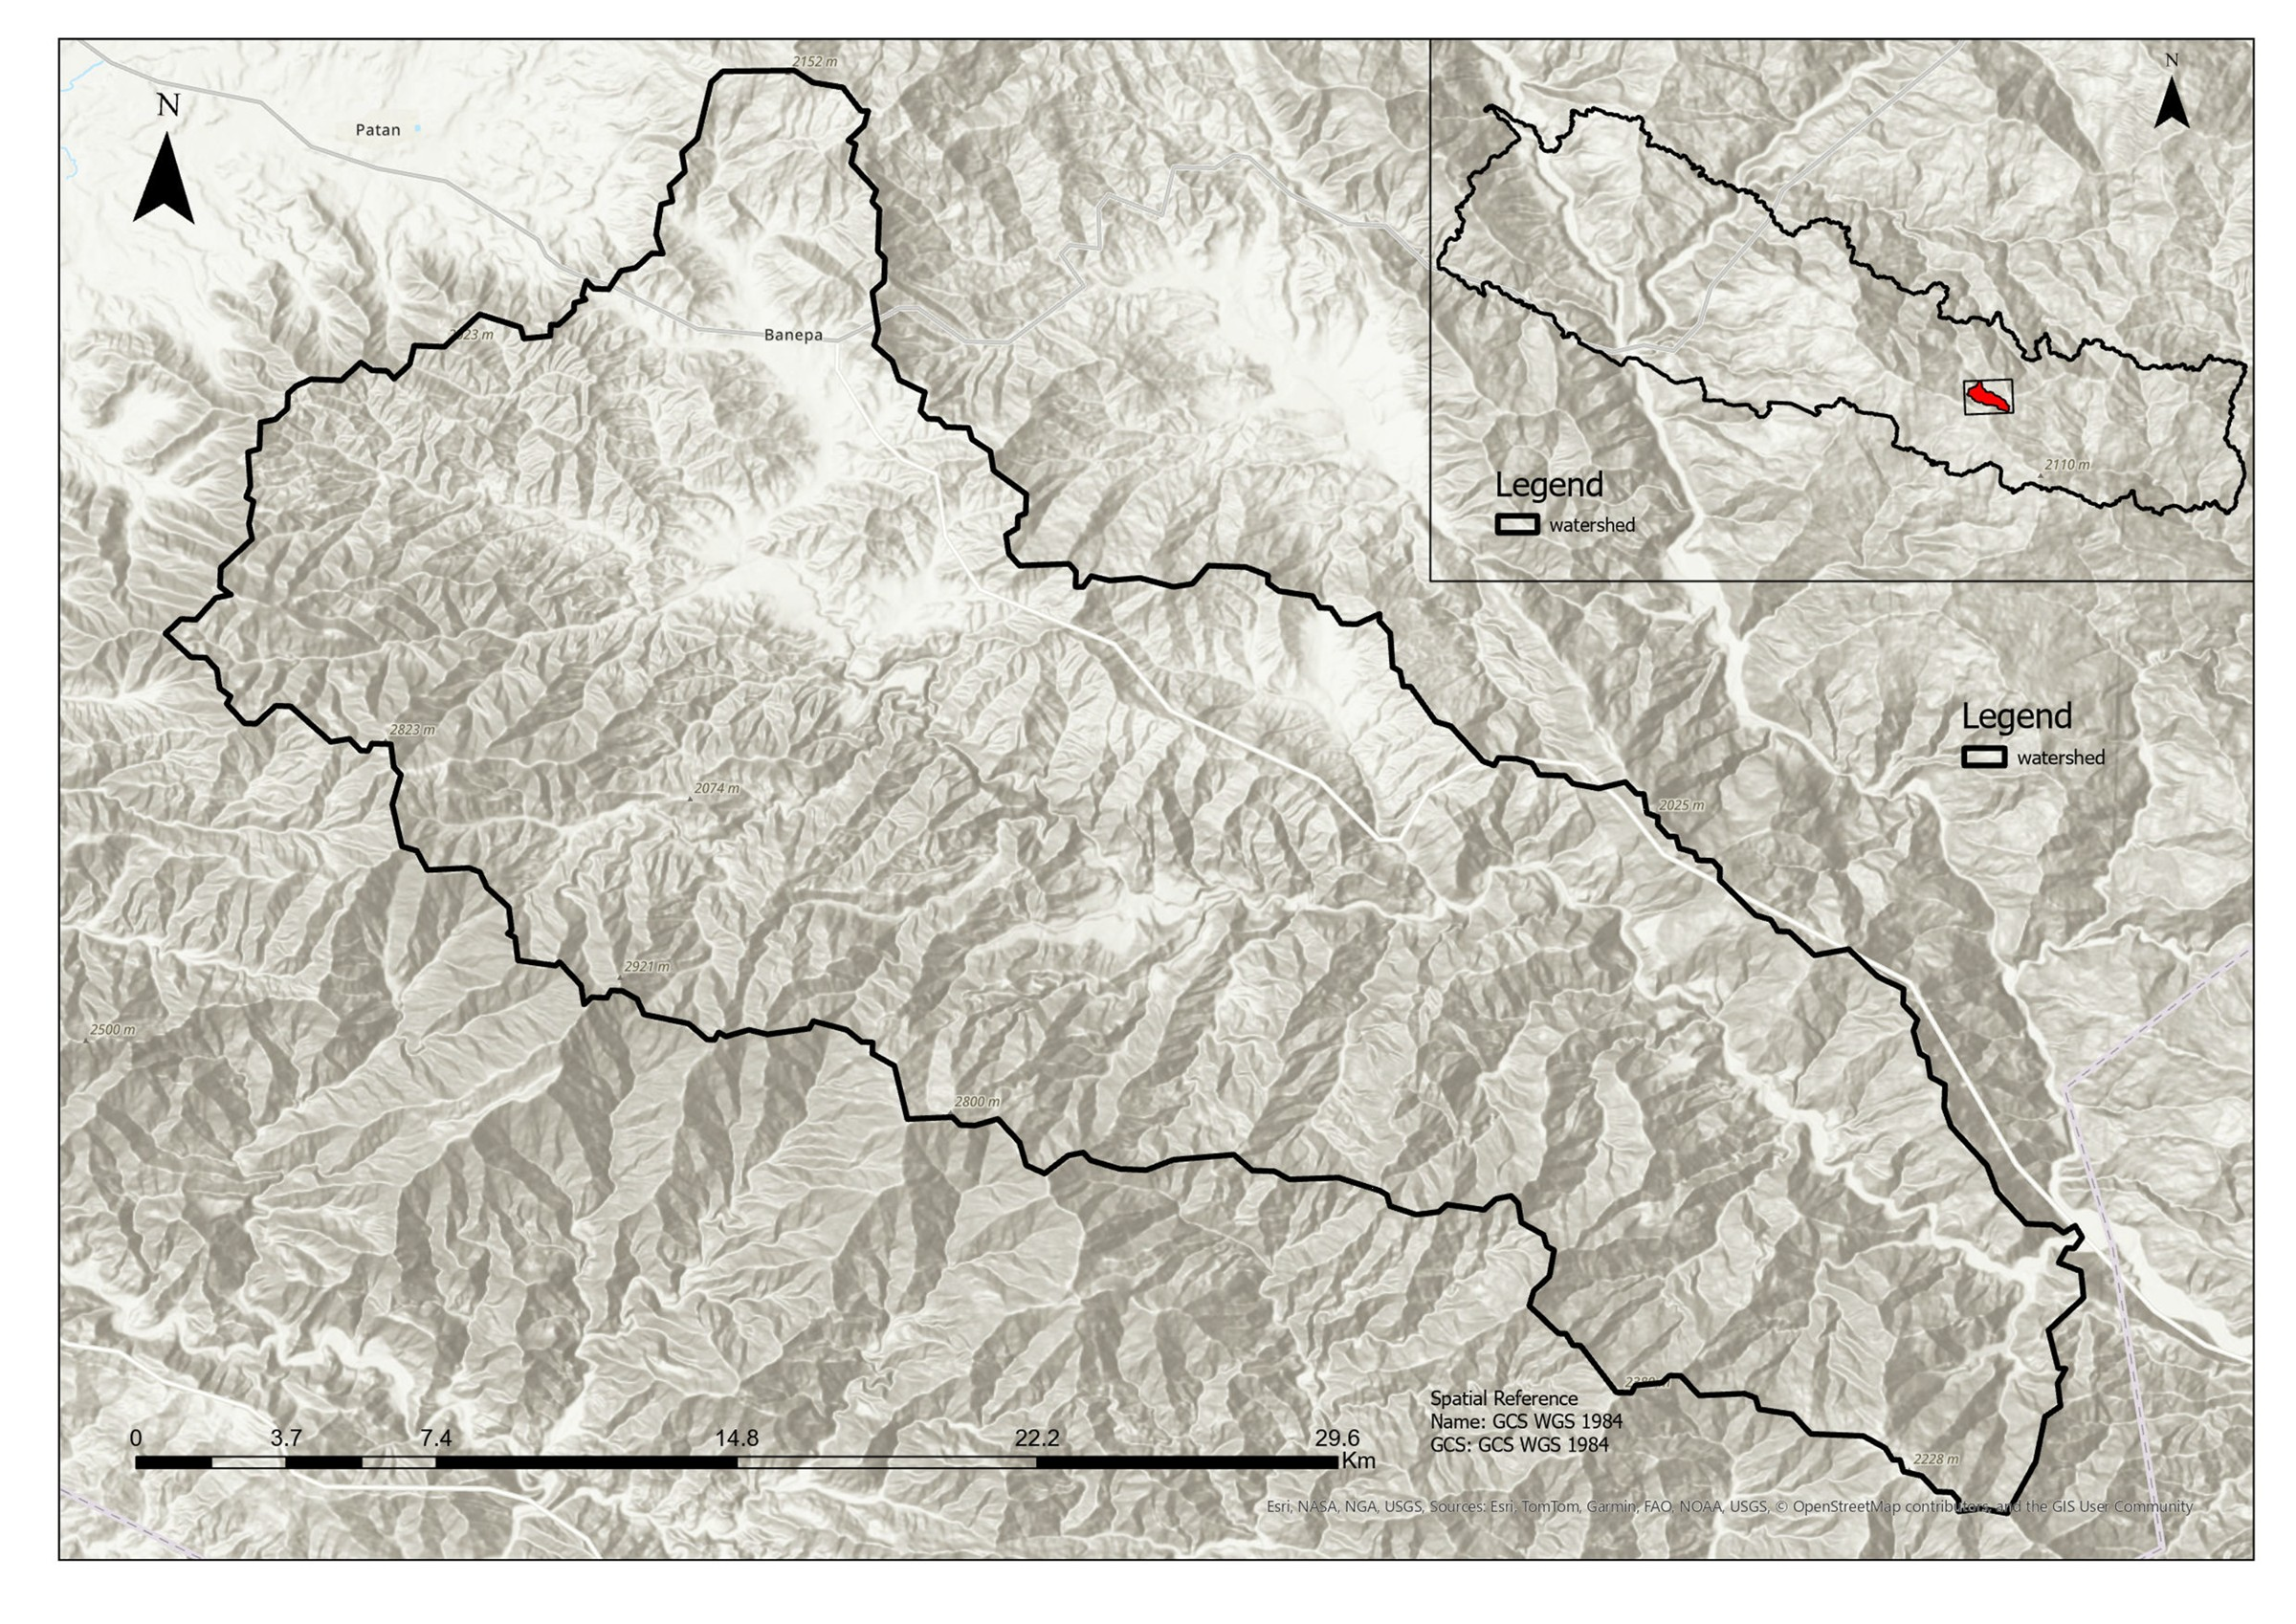
\includegraphics[width=0.95\linewidth]{figures/fig01_study_area_map}
\caption{Roshi Khola watershed boundary and location within Nepal (inset).}
\label{fig:map}
\end{figure}

Springs were assigned to the Roshi watershed using a spatial join against the watershed boundary polygon, since this boundary cuts across municipal administrative limits. Table~\ref{tab:inventory} summarises the inventory. The published description of the inventory reports 5,689 water sources, including 5,168 springs and 521 ponds \citep{pandit2026}; the survey export used in this project contains 5,692 records (5,170 springs and 522 ponds). After spatial filtering to the Roshi watershed and data-quality screening, 3,287 springs were retained as the analysis dataset. The other 2,056 springs of the inventory are not used anywhere in this report and are reserved for the staged generalisability testing of the dissertation phase.

\begin{table}[htbp]
\centering
\small
\caption{Spring inventory and analysis dataset}
\label{tab:inventory}
\begin{tabularx}{\linewidth}{LR}
\toprule
\textbf{Item} & \textbf{Count} \\
\midrule
Records in the survey export (springs and ponds) & 5,692 \\
Spring records & 5,170 \\
Pond records (not analysed) & 522 \\
Springs in the Roshi Khola analysis dataset & 3,287 \\
Active / dried springs in the analysis dataset & 2,560 / 727 \\
Springs outside the analysis dataset (reserved) & 2,056 \\
\bottomrule
\end{tabularx}
\end{table}

\subsection{Spring inventory}\label{sec:inventory}

The inventory was collected by trained community resource persons with a mobile survey application, and the dataset is publicly available through ICIMOD's Regional Database System \citep{thapa2025}. It records the location and condition of each spring (active or dried) and, for dried springs, the year of drying. Most records are dated between 2023-12-18 and 2024-04-18 (5th to 95th percentile of the record dates; 86\% of dated records are from 2024), so spring status describes conditions at the end of 2023 and in early 2024.

The raw survey records the drying year in the Bikram Sambat calendar. In the analysis table it was converted to the Gregorian (AD) calendar and stored in a column named \emph{Dried since how many years?}, which in fact holds the calendar year of drying. For 721 of the 723 dried springs with a recorded year, the difference between the two calendars is exactly 57 years; the remaining entries are inconsistent and are treated as data-entry errors. Drying years range from 1943 to 2023 (median 2015); 4 dried springs have no recorded year, and 241 (33.1\%) report 2015.

Of the 3,287 springs, 2,560 (77.9\%) are active and 727 (22.1\%) are dried; 2,784 (84.7\%) are classified as perennial and 503 (15.3\%) as seasonal. The perennial/seasonal classification is informative but not deterministic: 15.5\% of perennial springs are dried, compared with 58.6\% of seasonal springs.

\textbf{Reported cause of drying.} The raw survey also records a \emph{Reason of drying} for each dried spring. Matching the dried springs of the analysis dataset to the survey by coordinates gave a cause for all 727 of them (Table~\ref{tab:cause}). Earthquake and drought are reported almost equally often, and 195 of the 229 earthquake-attributed springs dried in 2015, the year of the Gorkha earthquake, which accounts for the spike of drying in that year (Figure~\ref{fig:cause}).

\begin{table}[htbp]
\centering
\small
\caption{Reported cause of drying for the dried springs of the analysis dataset (Drought includes \emph{Reduced Precipitation})}
\label{tab:cause}
\begin{tabularx}{\linewidth}{LRR}
\toprule
\textbf{Reported cause} & \textbf{Dried springs} & \textbf{Share of dried (\%)} \\
\midrule
Earthquake & 229 & 31.5 \\
Drought & 226 & 31.1 \\
Infrastructure development & 105 & 14.4 \\
Source neglected or disrupted & 95 & 13.1 \\
Natural disaster & 64 & 8.8 \\
Land use (deforestation, plantation) & 5 & 0.7 \\
Unknown & 3 & 0.4 \\
\bottomrule
\end{tabularx}
\end{table}

\begin{figure}[htbp]
\centering
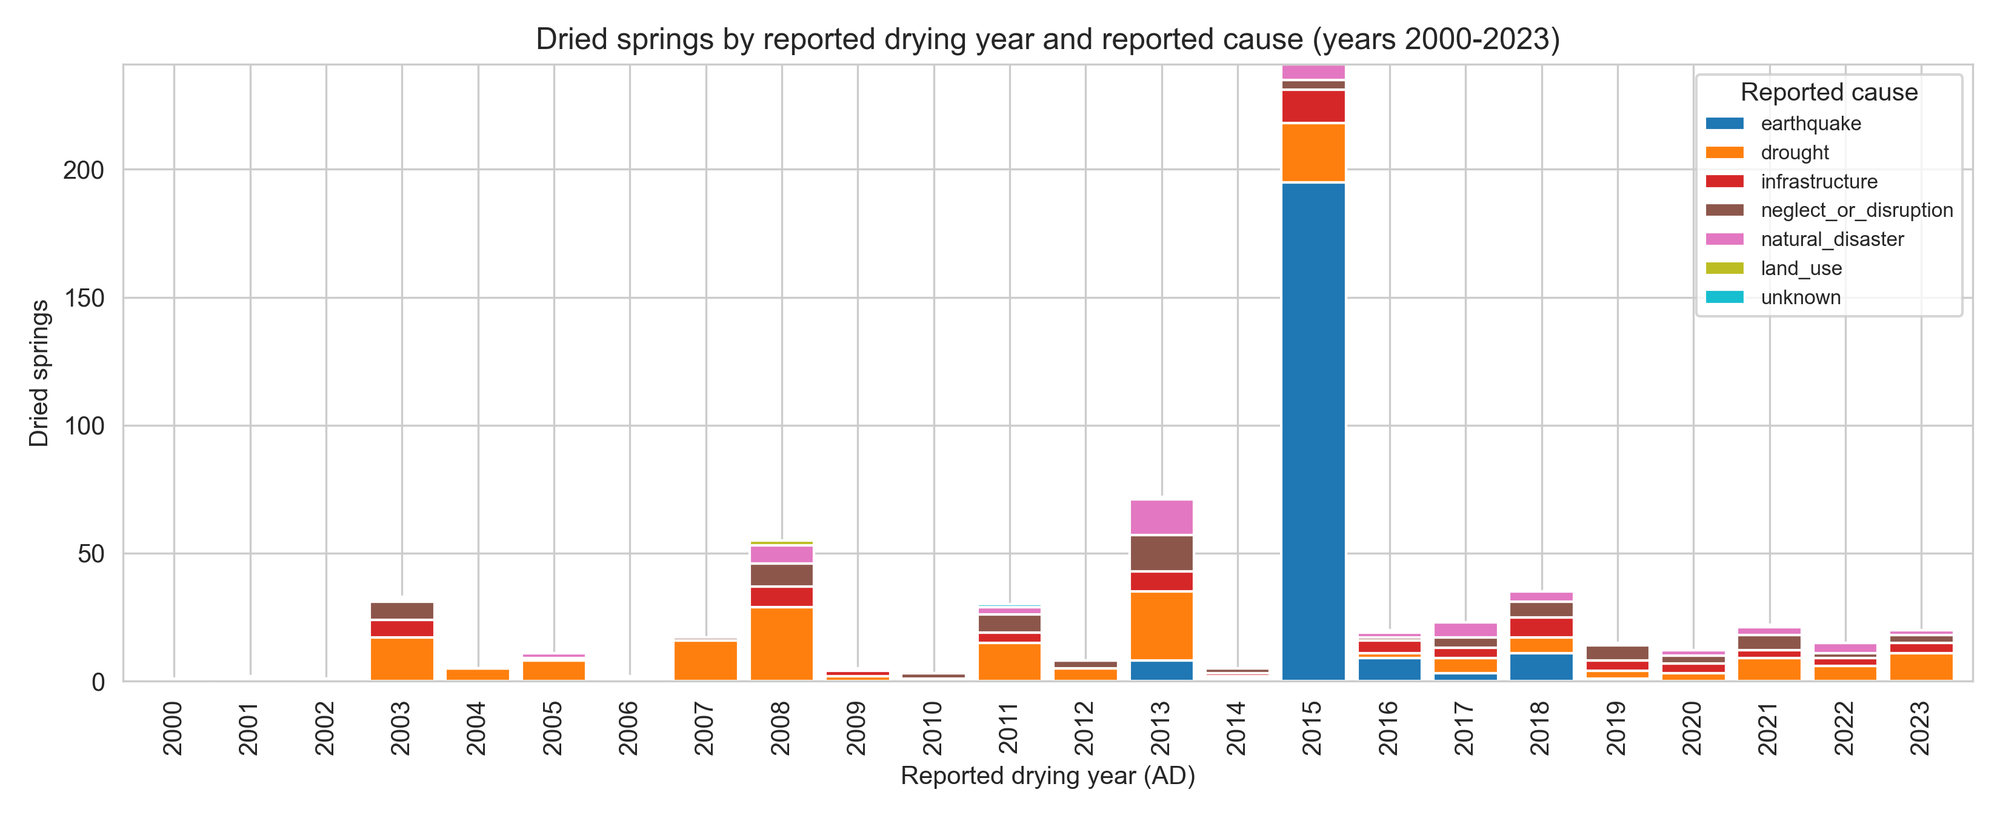
\includegraphics[width=0.95\linewidth]{figures/fig02_overview_drying_year_by_cause}
\caption{Dried springs by reported drying year (2000 to 2023) and reported cause.}
\label{fig:cause}
\end{figure}

\subsection{Watershed boundary and spatial harmonisation}

A watershed boundary polygon was used to constrain all analysis to the target basin. Spring occurrence and behaviour are governed by catchment-scale hydrological processes; springs outside the basin are subject to different recharge regimes, and including them would introduce spatial heterogeneity unrelated to the study objective. All vector and raster datasets were projected into a common coordinate reference system before any overlay or extraction, because projection mismatches can shift point locations relative to raster cells or polygons and produce incorrect attribute assignments \citep{zandbergen2009}.

Two data-quality observations bear on the evaluation. 51 springs share exact coordinates with another spring, and 36 rows are identical on all attributes; such duplicates can fall on both sides of a random train/test split. In the Model 3 split, 22 test springs (3 of them dried) share coordinates with a training spring, and leaving them out leaves the test ROC-AUC unchanged (0.748 against 0.748), so the duplicates do not inflate the reported performance.

\subsection{Topographic data (SRTM DEM)}\label{sec:topo}

Topographic information was derived from the SRTM digital elevation model \citep{farr2000,yang2011}. Topography is one of the most important controls on groundwater emergence in mountainous terrain \citep{forster1988,condon2015,broxton2009}: elevation influences recharge zones and vertical climatic gradients; slope affects infiltration opportunity and runoff; and aspect controls solar exposure, evapotranspiration demand and local moisture conditions \citep{gutierrez2013}. Elevation was extracted at each spring's coordinates, and slope (S) and aspect (A) were derived from the elevation surface:

\begin{equation}
S = \arctan\left(\sqrt{\left(\frac{\partial z}{\partial x}\right)^2 + \left(\frac{\partial z}{\partial y}\right)^2}\right)
\end{equation}

\begin{equation}
A = \arctan\left(\frac{\partial z/\partial y}{\partial z/\partial x}\right)
\end{equation}

where $\partial$z/$\partial$x and $\partial$z/$\partial$y are the rates of change of elevation in the east-west and north-south directions. Aspect was also grouped into eight 45\textdegree{} classes (N, NE, E, SE, S, SW, W, NW) and expressed as one-hot indicators. The slope was stored as \texttt{Slope\_\allowbreak{}sin} and \texttt{Slope\_\allowbreak{}cos}. However, \texttt{Slope\_\allowbreak{}sin} lies between 0.999999 and 1.0 for every spring, which corresponds to a slope of about 90\textdegree{} everywhere and indicates an error in the slope derivation (for example, slope computed on a DEM in geographic degrees without metre scaling). The slope variables therefore carry no information and are not interpreted in this report. Elevation, slope and aspect are not predictors in the proposal-compliant models.

Springs are concentrated at mid-elevations (median 1533 m; 1,820 of 3,287 springs lie between 1,400 and 1,700 m; Figure~\ref{fig:elev}). The share of dried springs decreases with elevation, from 33.6\% below 1,000 m and 30.6\% between 1,000 and 1,400 m to 22.0\% between 1,400 and 1,700 m and 13.4\% between 1,700 and 2,000 m (17.2\% above 2,000 m, where springs are few). By aspect, the share of dried springs is lowest on east- and north-east-facing slopes (13.8\% and 14.2\%) and highest on south-west-, south- and west-facing slopes (31.9\%, 29.7\% and 29.5\%; Figure~\ref{fig:aspect}, Figure~\ref{fig:polar}).

\begin{figure}[htbp]
\centering
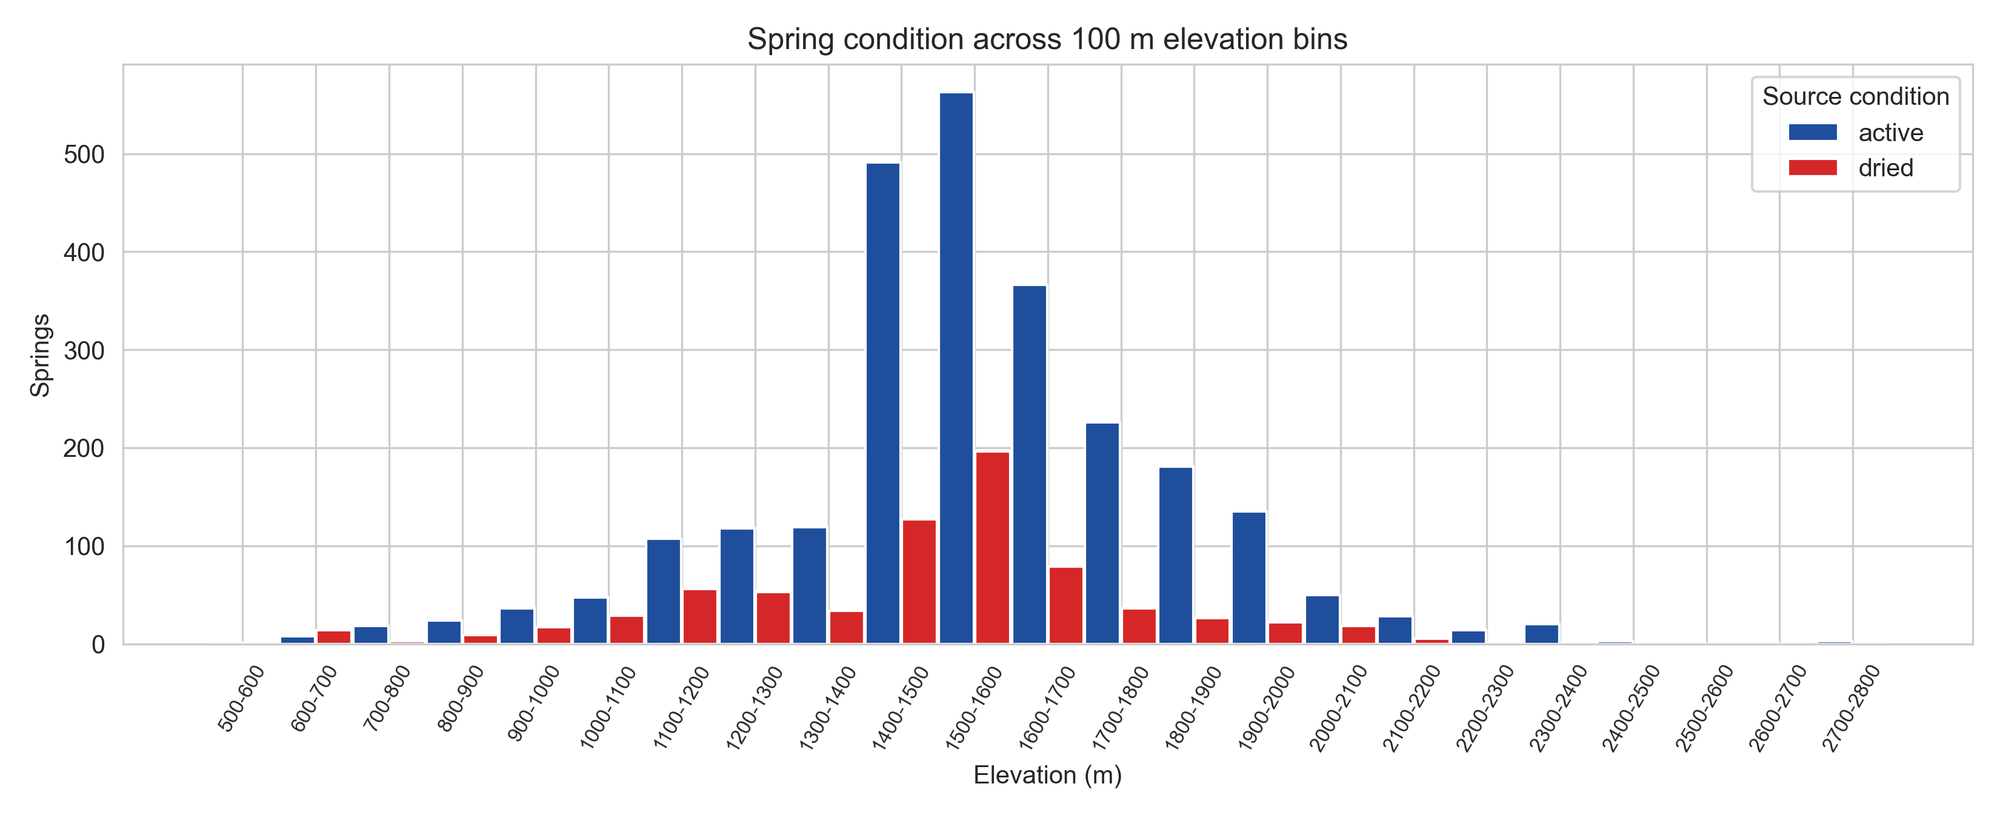
\includegraphics[width=0.95\linewidth]{figures/fig03_overview_elevation_bins}
\caption{Spring condition across 100 m elevation bins.}
\label{fig:elev}
\end{figure}

\begin{figure}[htbp]
\centering
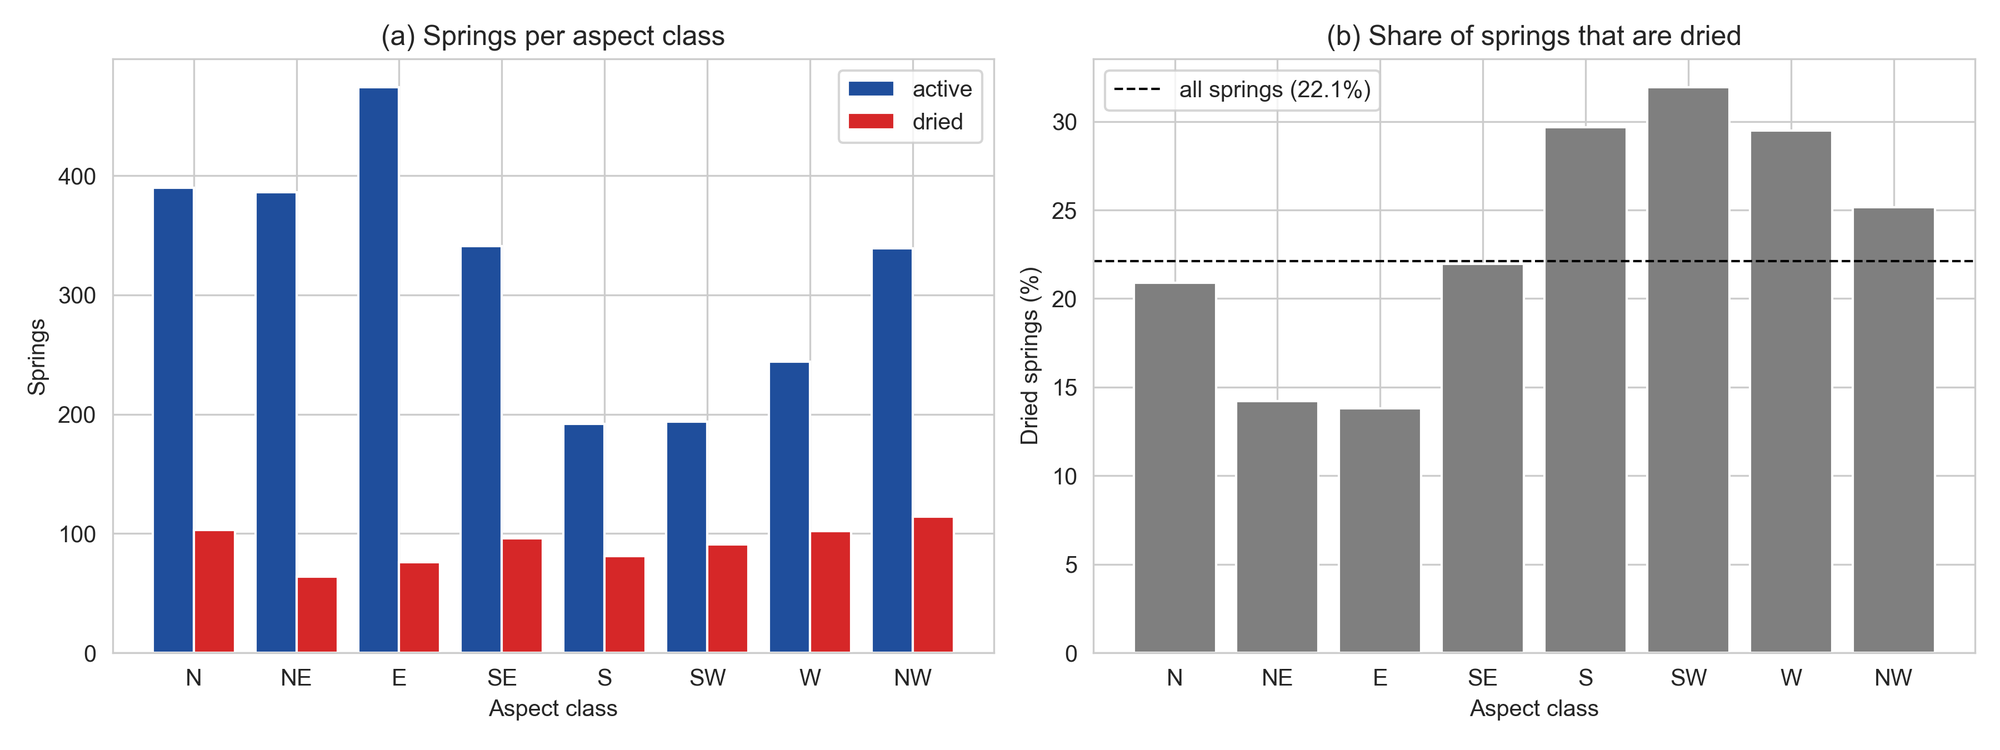
\includegraphics[width=0.95\linewidth]{figures/fig04_overview_aspect}
\caption{(a) Active and dried springs per aspect class; (b) share of springs in each aspect class that are dried, with the overall share as a dashed line.}
\label{fig:aspect}
\end{figure}

\begin{figure}[htbp]
\centering
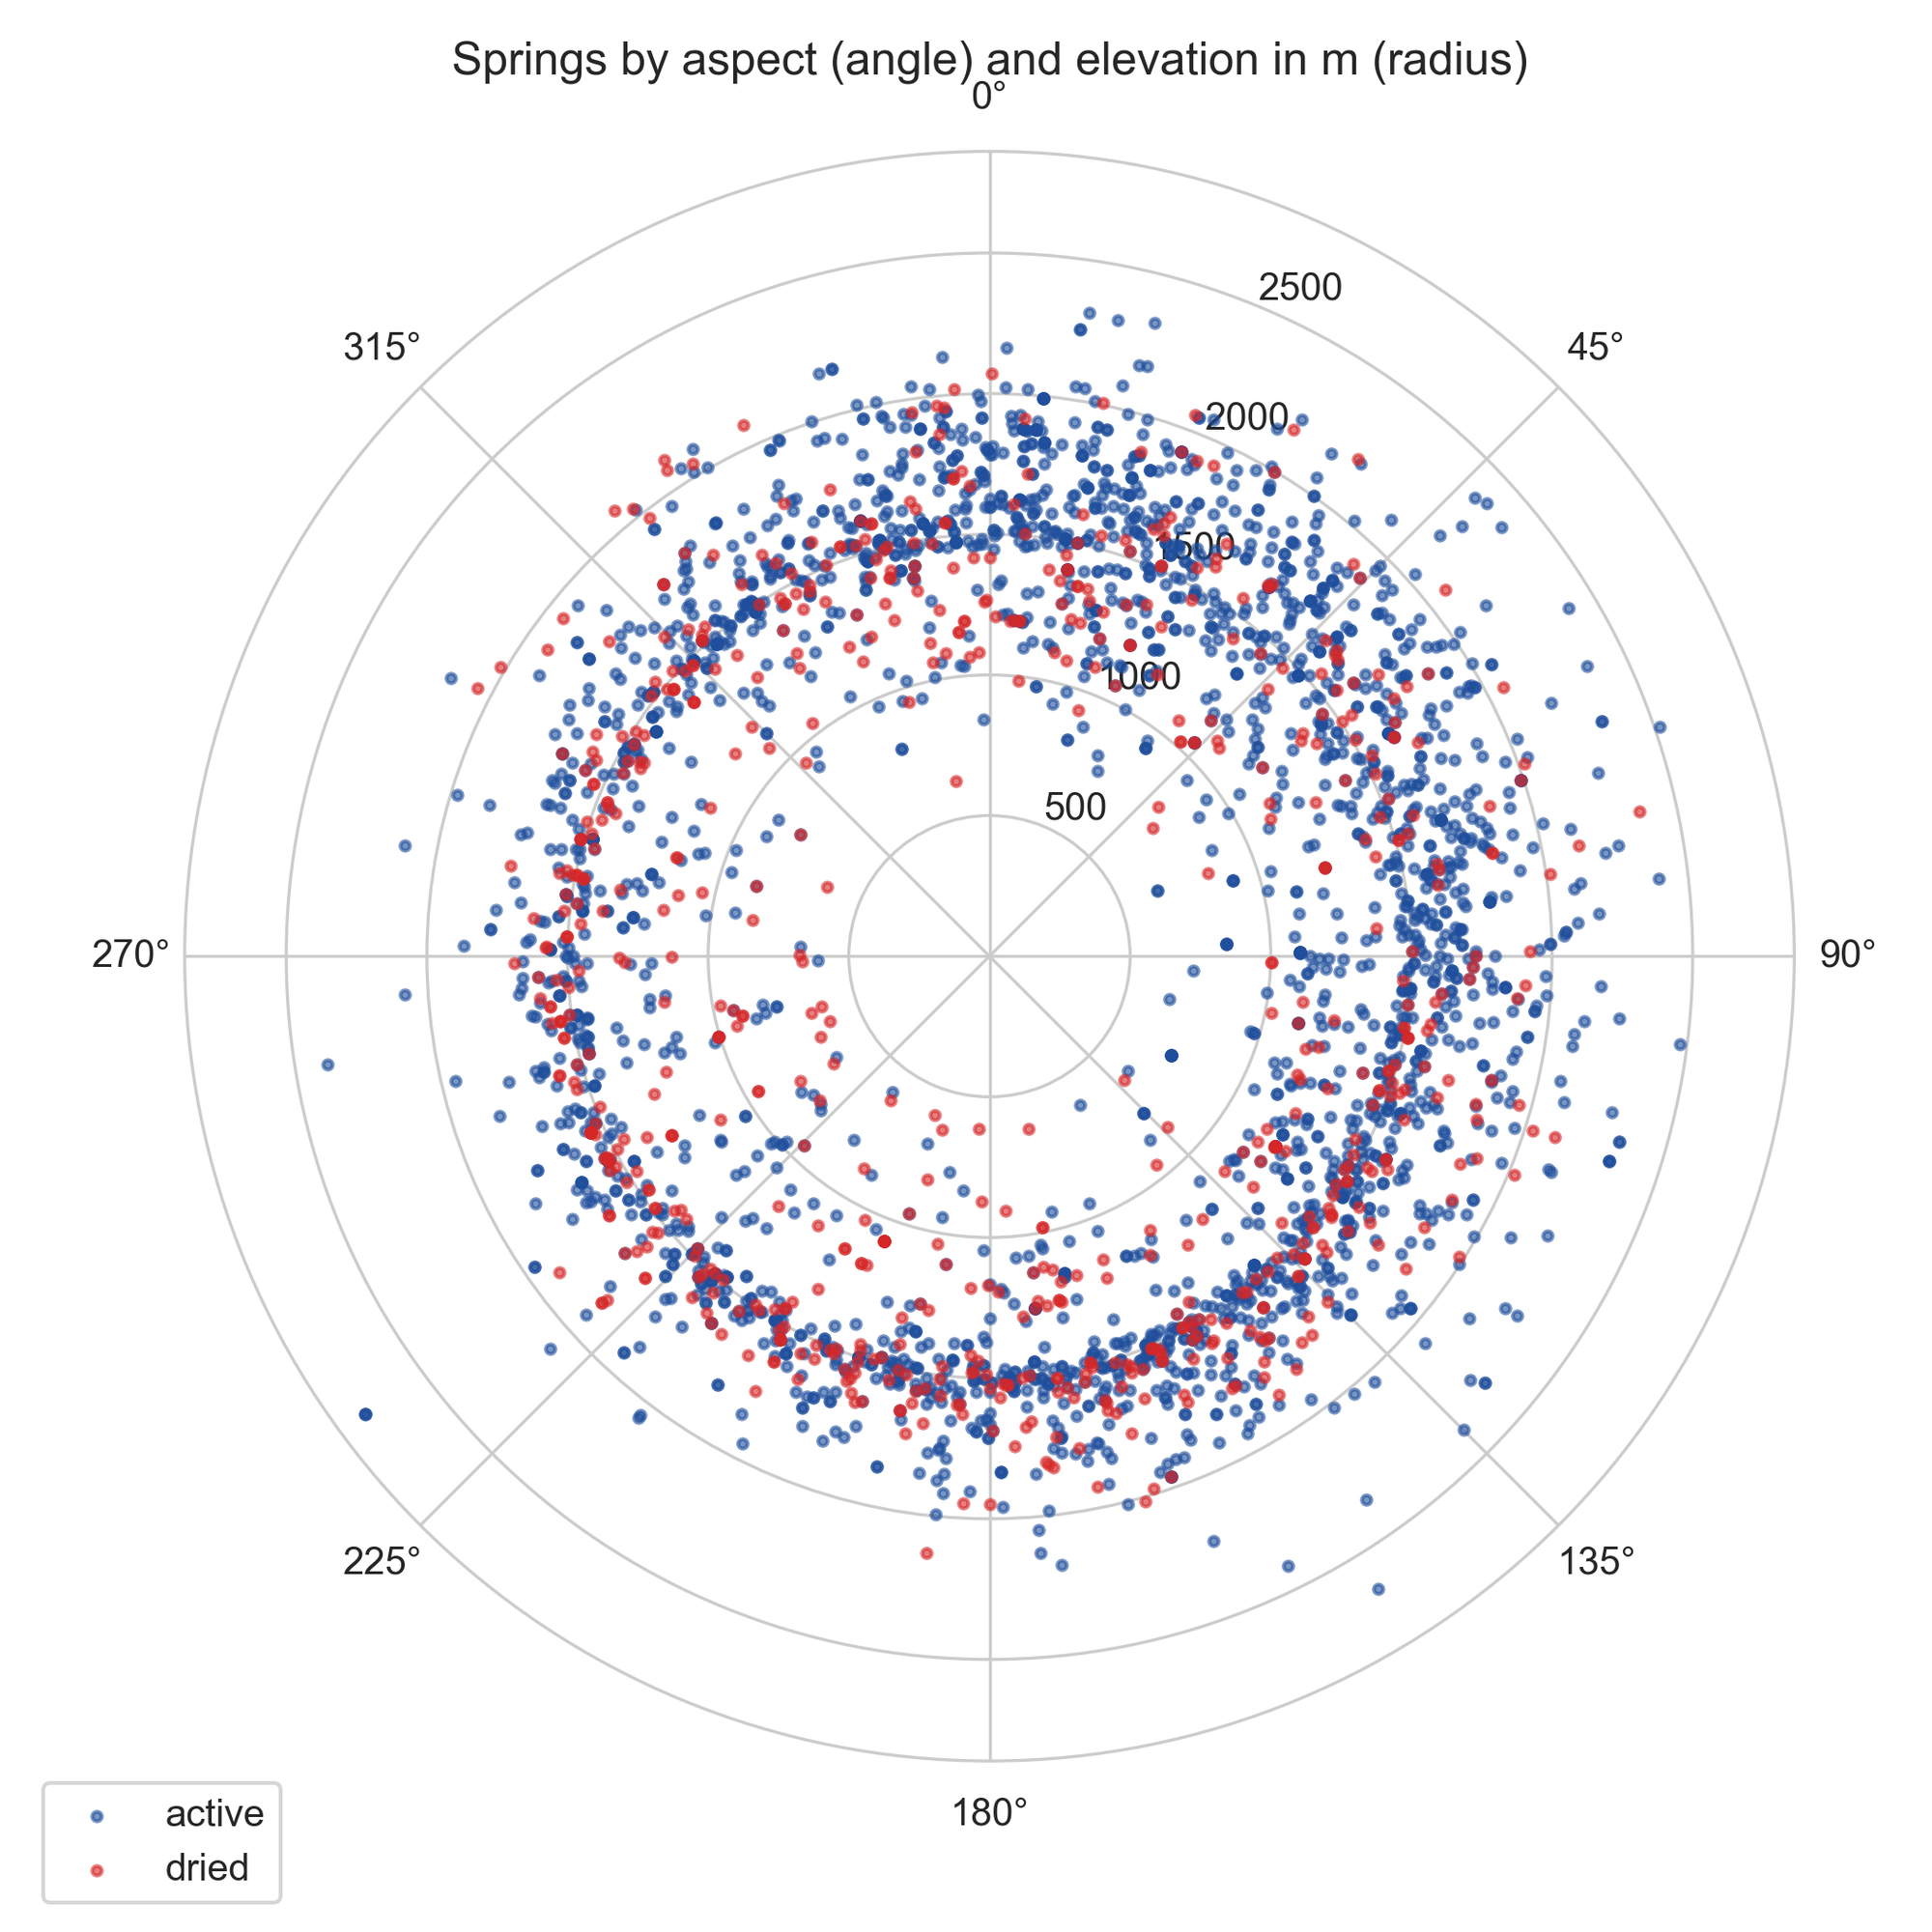
\includegraphics[width=0.65\linewidth]{figures/fig05_overview_elevation_aspect_polar}
\caption{Active and dried springs by aspect (angle, north at the top) and elevation (radius, m).}
\label{fig:polar}
\end{figure}

\subsection{Land use and land cover (ICIMOD)}\label{sec:lulc}

The ICIMOD regional land-cover product was used to characterise the surroundings of each spring. Land cover influences infiltration, evapotranspiration, soil-moisture retention, runoff generation and human disturbance \citep{jayawickreme2007,bosmans2017}, and in mountain environments it reflects slope modification, deforestation and cultivation pressure that affect spring recharge \citep{pant2026}. Land cover was summarised within a 1 km buffer around each spring rather than at the spring point, because spring discharge is influenced by a contributing area wider than the emergence point \citep{dreiss1983}. Within each buffer, pixel counts per class were converted to percentage cover. For dried springs, the land-cover year closest to the reported drying year was used.

Land cover is excluded as a modelled predictor for two reasons. Future land-cover datasets corresponding to the SSP scenarios planned for the dissertation are unavailable, which would make historical training and future projection data inconsistent. In addition, the historical product covers only 2000 to 2022, so springs that dried before 2000 cannot be assigned a representative land-cover condition, and the missing values would be correlated with the label. Land cover is retained as contextual background only.

\subsection{Geological data}\label{sec:geology}

Geological and lithological attributes were extracted from the geological map of the study area. Spring occurrence is controlled by rock type, fracture density, permeability and the contrast between aquifers and aquitards \citep{ra2018,doctor2008}. Each spring was spatially joined to the geological polygon in which it occurs, and the corresponding formation and rock type were assigned as categorical attributes (26 springs have no formation). Geological variables were not used as predictors because the mapped formations are coarse and extend over large areas, leaving many neighbouring springs with identical geological attributes.

\subsection{Road and infrastructure data}\label{sec:roads}

Road construction can alter slope stability, intercept shallow groundwater, redirect runoff and fragment recharge areas \citep{dutton2005,montgomery1994}. Roads were analysed within a 1 km buffer around each spring and counted by eight compass sectors (\texttt{Road-N} to \texttt{Road-NW}), since roads upslope, downslope or lateral to a spring may have different hydrological effects. Dried springs have a higher mean number of road crossings than active springs in 7 of the 8 directions (all except north), and a higher mean total (1.93 against 1.66 crossings; Figure~\ref{fig:roads}). These are descriptive associations, not evidence of an independent or causal effect, and road variables are not predictors in the proposal-compliant model.

\begin{figure}[htbp]
\centering
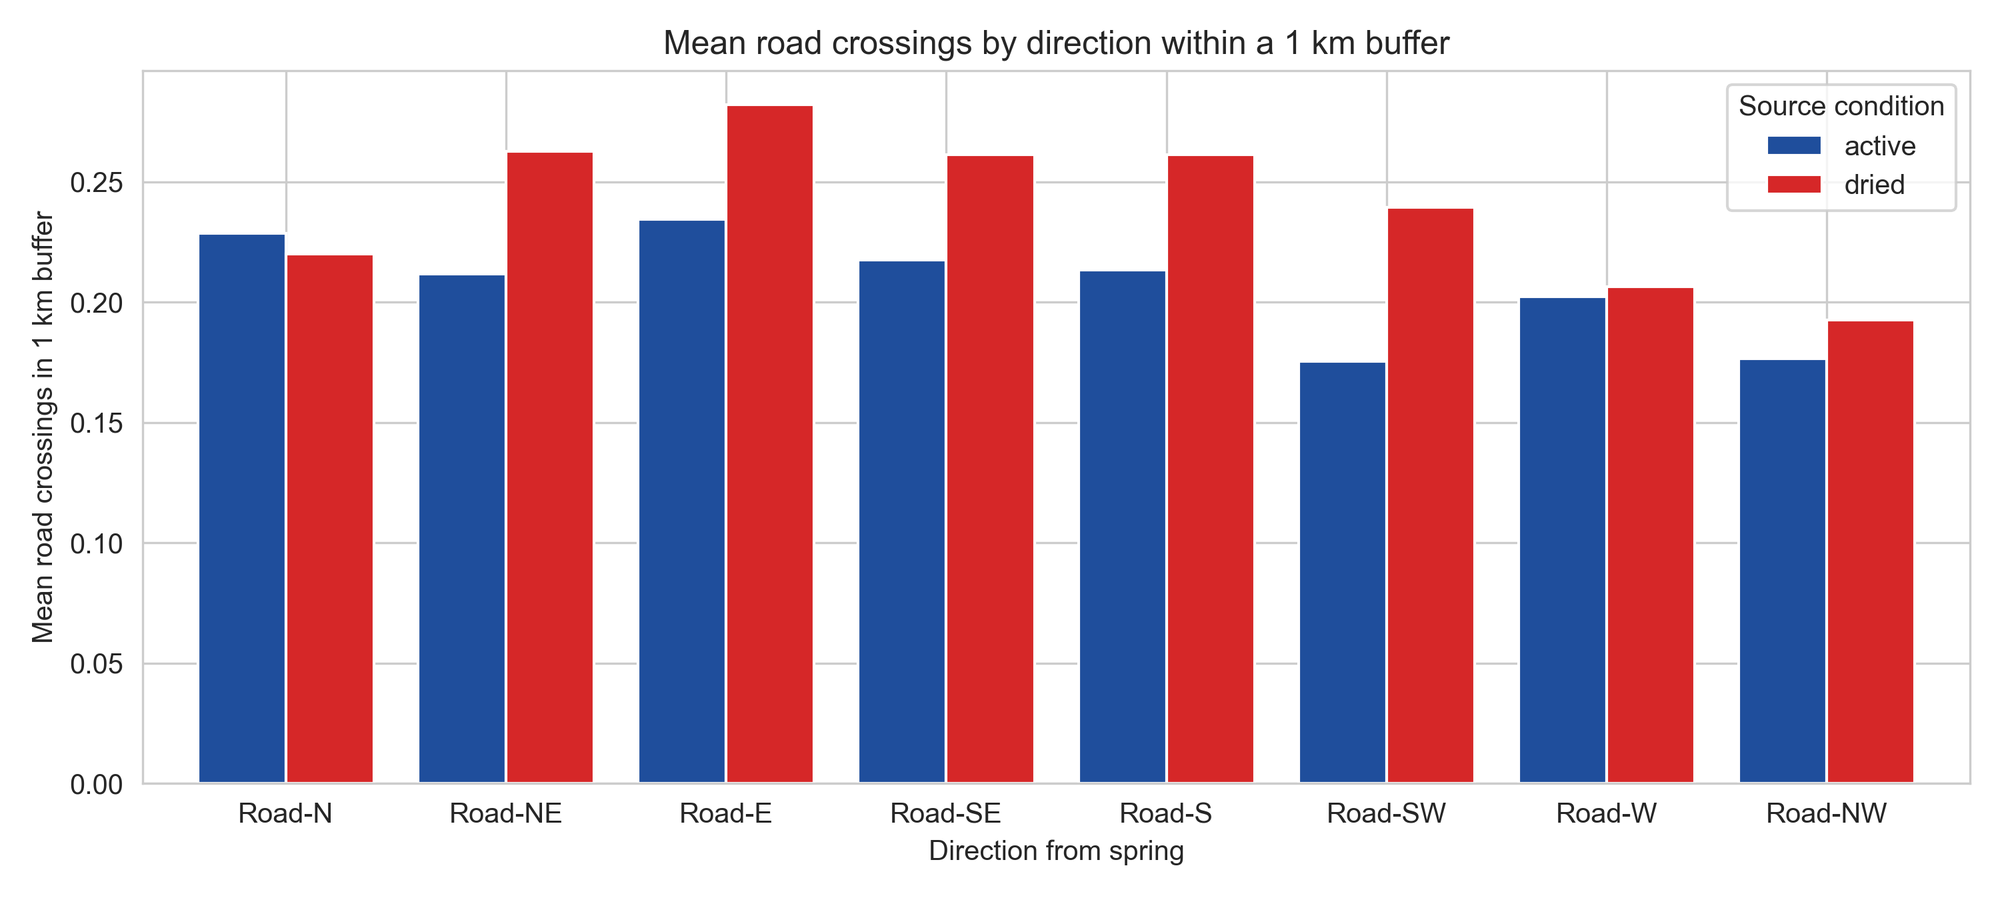
\includegraphics[width=0.9\linewidth]{figures/fig06_overview_road_crossings}
\caption{Mean road crossings within a 1 km buffer by direction for active and dried springs.}
\label{fig:roads}
\end{figure}

\subsection{Climate reanalysis data (ERA5-Land)}\label{sec:era5}

Climate data were obtained from the ERA5-Land reanalysis \citep{munozsabater2021}, the land-surface component of ERA5 \citep{hersbach2020}. The NetCDF file used covers 1950-01 to 2026-04 (916 monthly time steps) on a 0.1\textdegree{} grid (about 9 to 11 km) over 0 to 40\textdegree{} N and 60 to 100\textdegree{} E, with four variables: 2 m air temperature (\texttt{t2m}), 2 m dewpoint temperature (\texttt{d2m}), total precipitation (\texttt{tp}) and potential evaporation (\texttt{pev}). The 3,287 springs fall within only 12 ERA5-Land grid cells (between 1 and 1,065 springs per cell), so all springs within a cell receive identical climate values. As discussed in Section~\ref{sec:lit-reanalysis}, these values represent regional climate forcing, with temperature more reliable than precipitation \citep{khadka2022,lavers2022}.

\subsubsection{Extraction and temporal aggregation}

For each spring, the nearest ERA5-Land grid cell was selected; nearest-cell extraction avoids interpolation artefacts and is reproducible. The monthly series were averaged to calendar years, using complete years only. Temperature and dewpoint were converted from kelvin to \textdegree{}C. Precipitation and potential evaporation, stored as monthly means of daily accumulations in metres, were converted to millimetres per year (multiplying by 1,000 and by 365). Potential evaporation was also multiplied by $-$1 to remove the ECMWF sign convention (negative values denote evaporation), so that larger values mean greater evaporative demand.

\subsubsection{Trend estimation and 15-year summary}

Temporal trends were estimated with the non-parametric Mann-Kendall test \citep{mann1945}, which detects monotonic trends without assuming a distribution, and their magnitude with Sen's slope \citep{sen1968}, the median of all pairwise slopes, which is insensitive to outliers. The slope, rather than its statistical significance, is used as the predictor because the aim is to encode the magnitude and direction of change at each location. The 15-year mean of each variable was computed over the same window. Each spring therefore has eight climate features: four trends (\texttt{Dewpoint\_\allowbreak{}rate}, \texttt{Temperature\_\allowbreak{}rate}, \texttt{Precipitation\_\allowbreak{}rate}, \texttt{Evaporation\_\allowbreak{}rate}) and four means (\texttt{Dewpoint\_\allowbreak{}mean}, \texttt{Temperature\_\allowbreak{}mean}, \texttt{Precipitation\_\allowbreak{}mean}, \texttt{Evaporation\_\allowbreak{}mean}).

\subsubsection{Climate window definition: two versions}\label{sec:windows}

\textbf{Version A (label-conditional window).} An active spring uses the 15 years ending in the survey year (2009 to 2023); a dried spring uses the 15 years ending at its own reported drying year. A complete window requires an end year of at least 1964 (ERA5-Land begins in 1950), so 5 springs that dried earlier and 4 dried springs without a recorded year have no Version A features, leaving 3,278 springs. The design was intended to describe each spring over the period most relevant to its status, but it leaks the label (Section~\ref{sec:leakage}).

\textbf{Version B (fixed window).} Every spring, active or dried, uses the same window (2009 to 2023), which ends in the survey year. The features then describe each location's recent climate independently of when or whether the spring dried. Using a common window for all classes follows the principle that predictor construction must not depend on information that is only known because the outcome is known \citep{kaufman2011}.

Figure~\ref{fig:windows} shows why the two versions behave so differently. Regional temperature varies from year to year and is higher in recent decades (the 2010s average 0.37 \textdegree{}C warmer than the 1950s across the 12 cells), while the windows of dried springs end in many different years, mostly before the survey year that ends every active spring's window.

\begin{figure}[htbp]
\centering
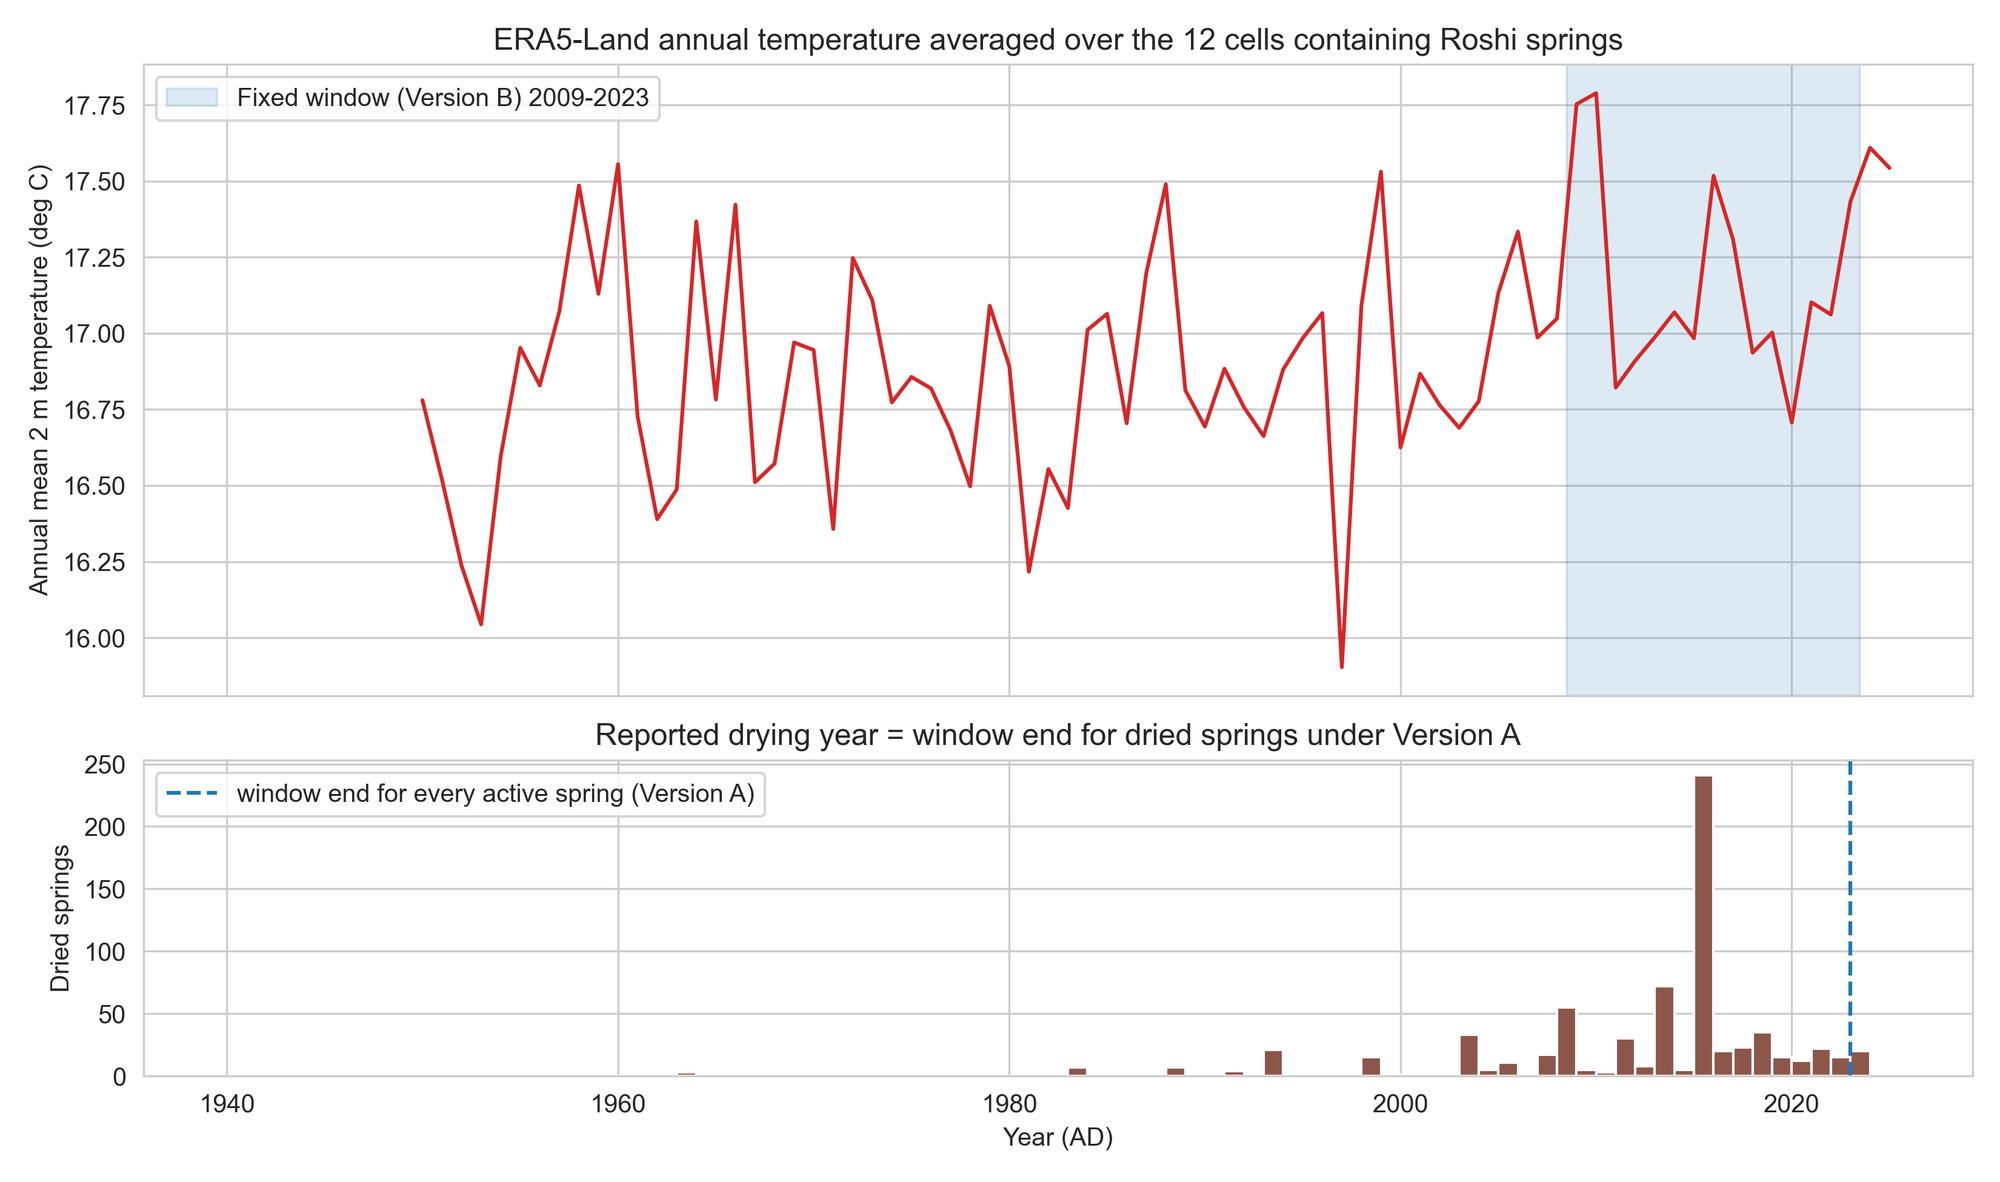
\includegraphics[width=0.95\linewidth]{figures/fig07_climate_timeseries_windows}
\caption{Top: ERA5-Land annual mean temperature averaged over the 12 cells containing Roshi springs, with the fixed Version B window shaded. Bottom: reported drying years, which set the end of the Version A window for dried springs.}
\label{fig:windows}
\end{figure}

Under Version A, the climate distributions of active and dried springs differ strongly, especially for the trends (Figure~\ref{fig:distA}). The median precipitation trend, for example, is 25.3 mm/yr per year for active springs but 0.9 for dried springs, and the median temperature trend is -0.0028 against 0.0190 \textdegree{}C per year. Under Version B the trend distributions of the two classes almost coincide (median precipitation trend 25.3 against 25.2; Figure~\ref{fig:distB}), while differences in the 15-year means remain (median temperature mean 16.52 \textdegree{}C for active and 17.33 \textdegree{}C for dried springs). Most of the separation seen under Version A is therefore a product of the window timing, not of climate at the springs. The submitted version of this report interpreted the Version A distributions as evidence of ``tipping points'' and of evaporative demand as ``the primary driver'' of drying; those interpretations are withdrawn.

\begin{figure}[htbp]
\centering
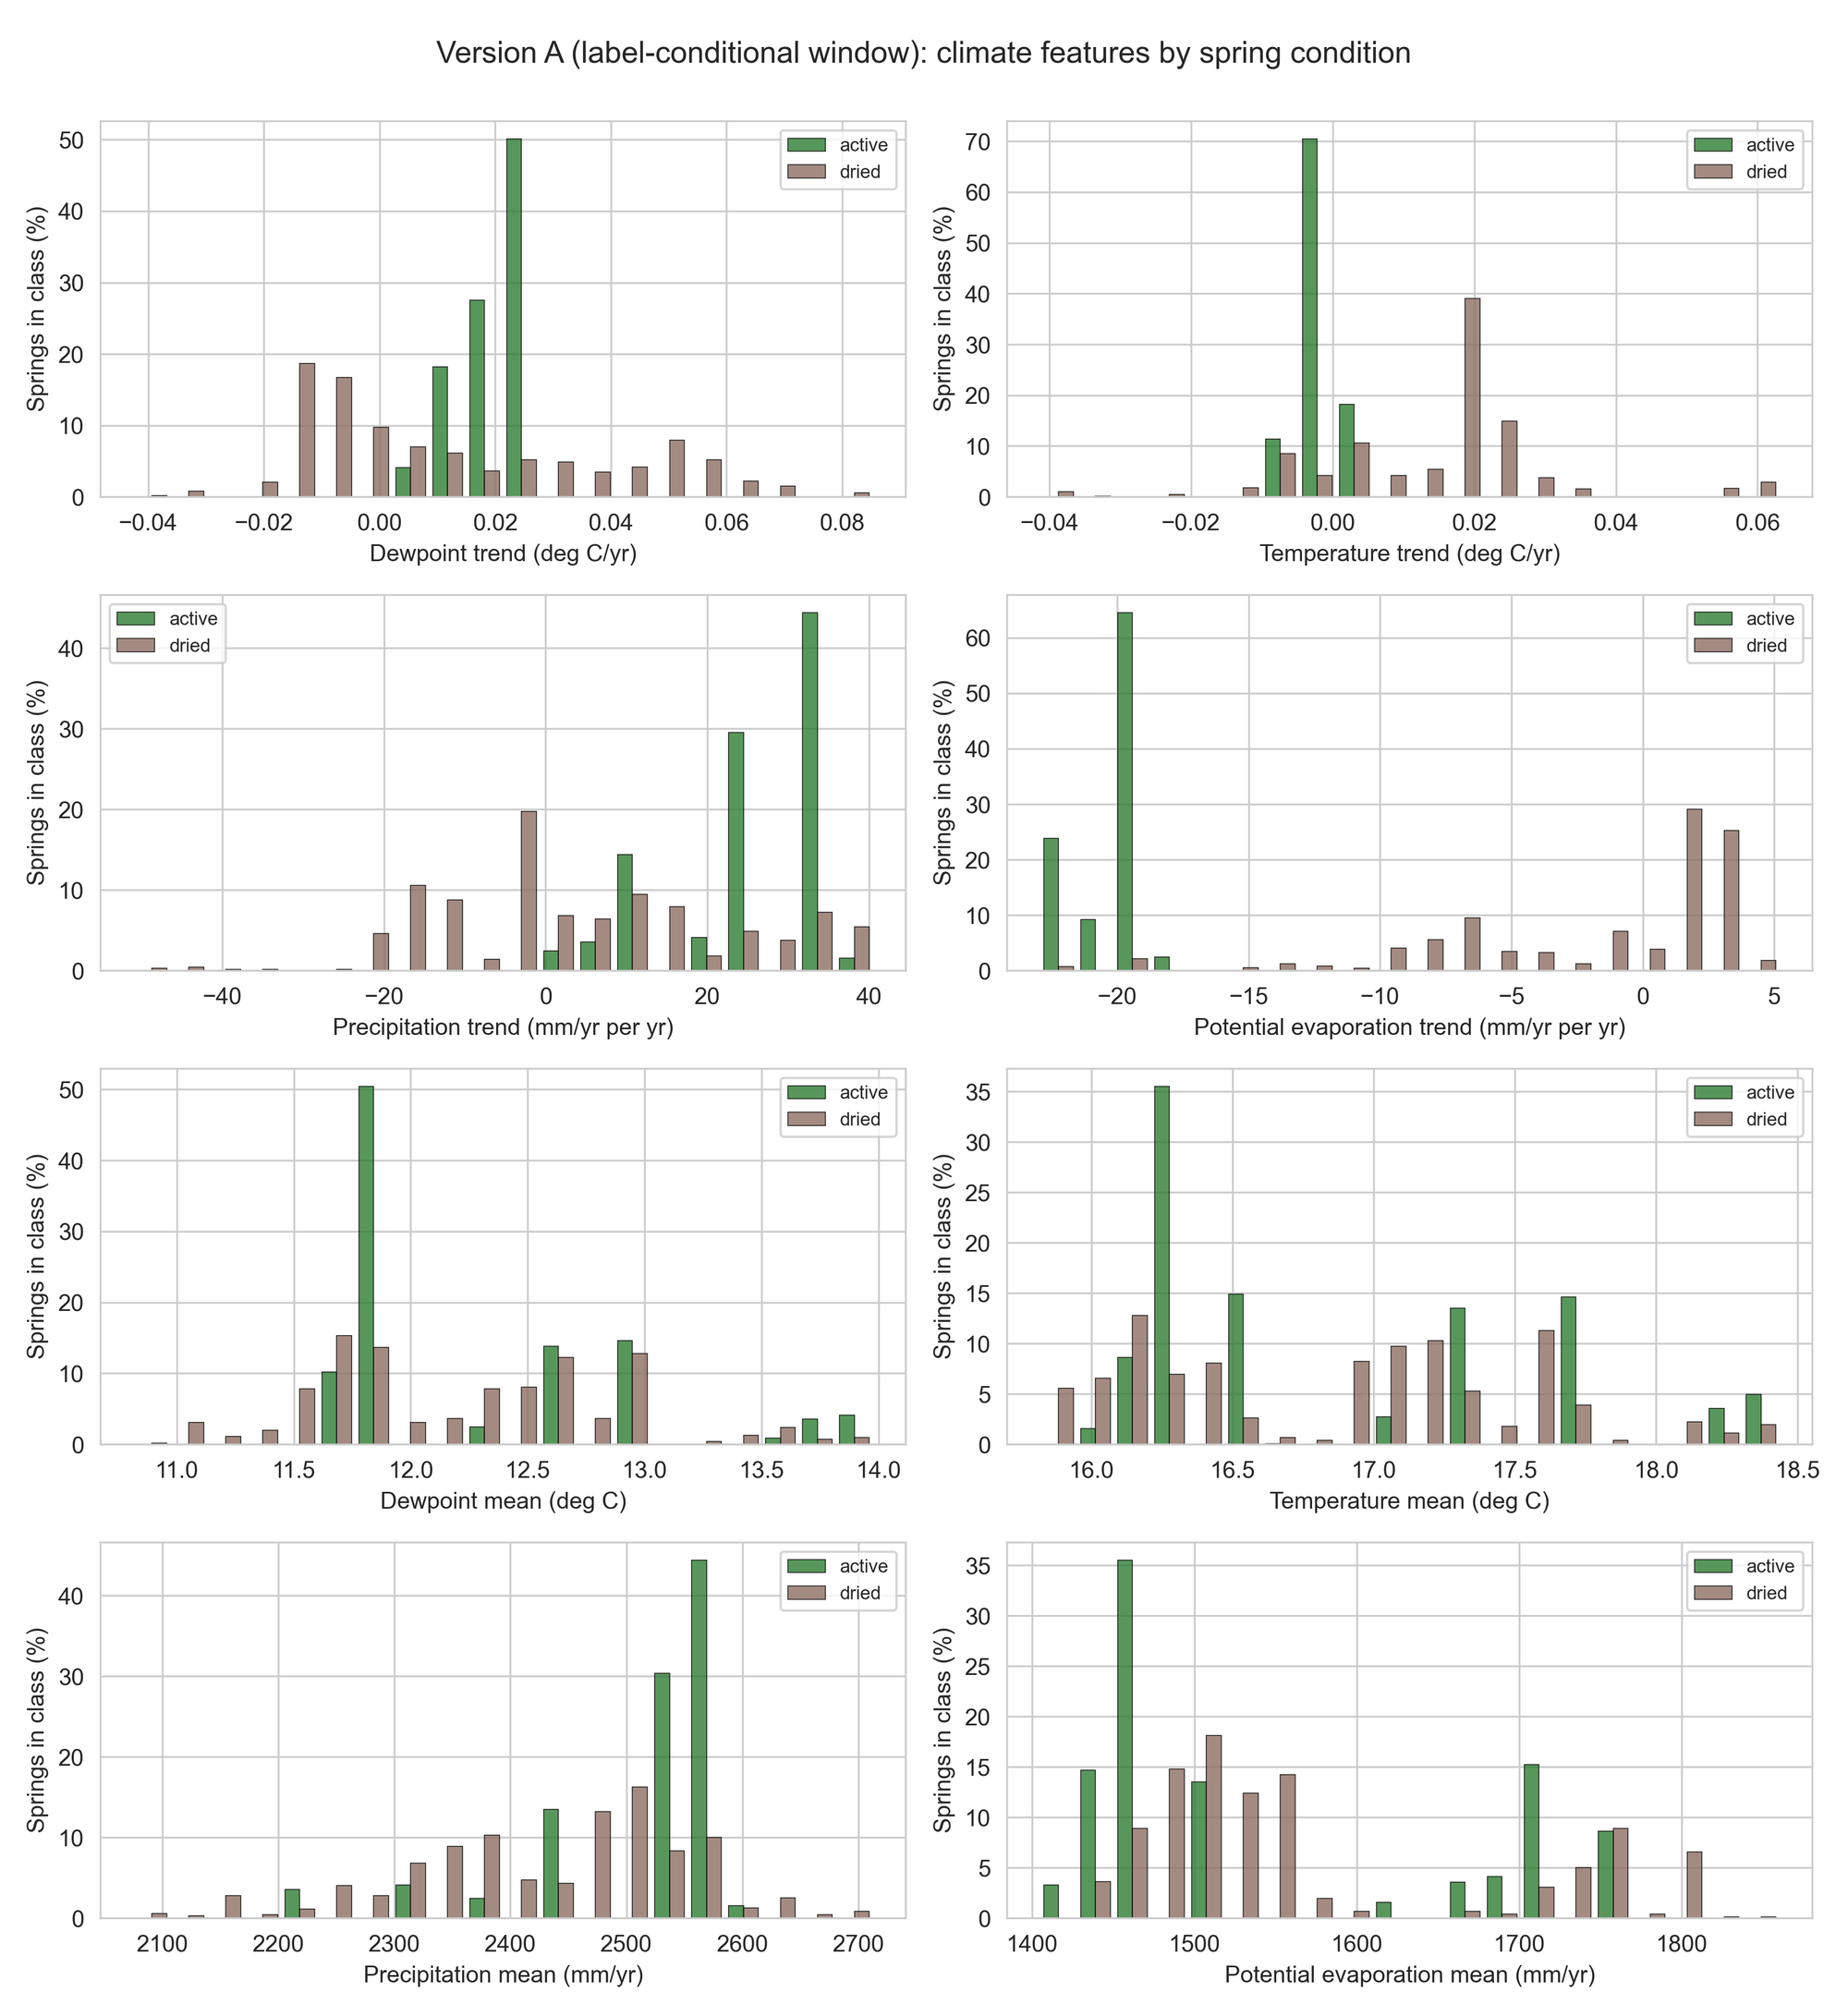
\includegraphics[width=0.85\linewidth]{figures/fig08_climate_distribution_version_a}
\caption{Climate features by spring condition under Version A (label-conditional window). Each class sums to 100\%.}
\label{fig:distA}
\end{figure}

\begin{figure}[htbp]
\centering
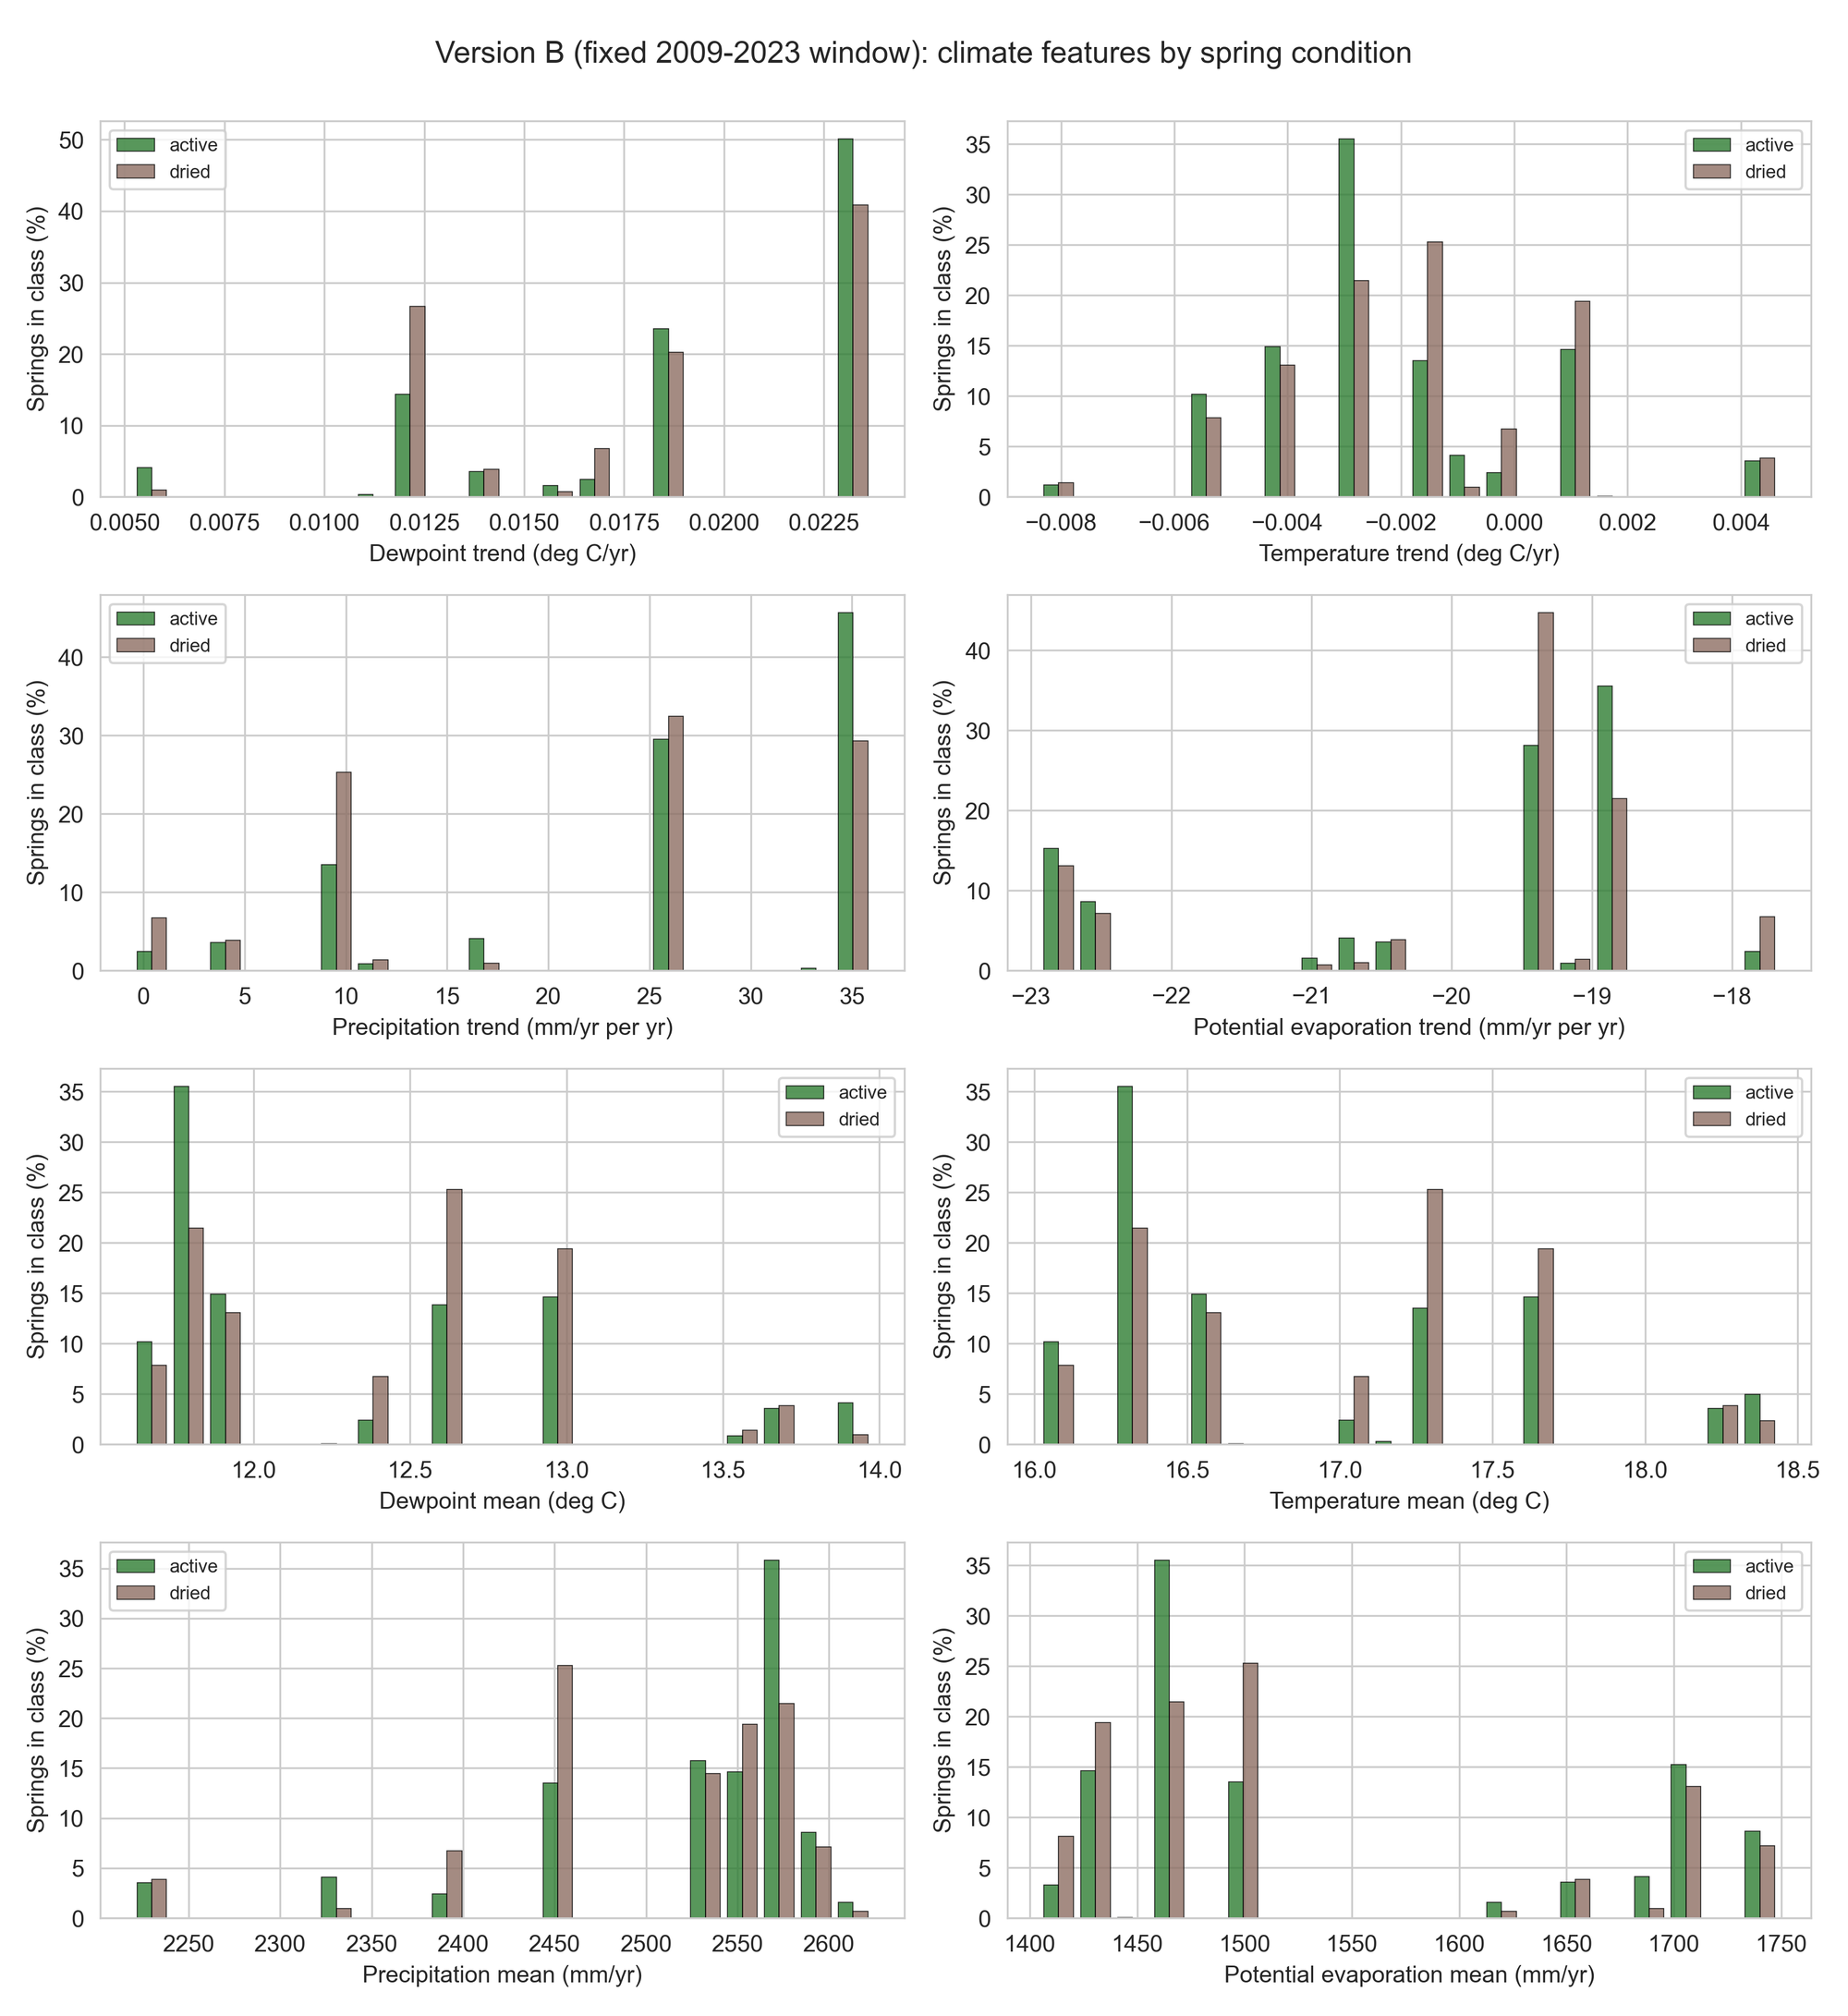
\includegraphics[width=0.85\linewidth]{figures/fig09_climate_distribution_version_b}
\caption{Climate features by spring condition under Version B (fixed window, 2009 to 2023). Each class sums to 100\%.}
\label{fig:distB}
\end{figure}

\subsection{Dataset assembly}\label{sec:assembly}

All layers were consolidated into one master table of 3,287 springs combining spring attributes, terrain derivatives, land-cover summaries, geological attributes, road-network counts and climate means and trends (Table~\ref{tab:datasets}). The climate features used in this report are recomputed by the project code for both window versions rather than taken from the master table (Appendix A).

\begin{table}[htbp]
\centering
\footnotesize
\caption{Datasets used to build the analysis table}
\label{tab:datasets}
\begin{tabularx}{\linewidth}{LLLLL}
\toprule
\textbf{Dataset} & \textbf{Spatial resolution} & \textbf{Temporal resolution} & \textbf{Key variables} & \textbf{Role in analysis} \\
\midrule
Spring inventory \citep{thapa2025} & Point & Single survey, 2023 to 2024 & location, condition, perennial/seasonal, drying year, reason of drying & Sample, labels and spring type \\
Watershed boundary & Polygon & Static & Roshi Khola basin outline & Restricts analysis to the catchment \\
SRTM DEM & Raster & Static & elevation & Elevation, slope, aspect (context) \\
ICIMOD land cover & Raster & Multi-year, 2000 to 2022 & land-cover classes & 1 km buffer composition (context) \\
Geological map & Polygon & Static & formation, rock type & Geology per spring (context) \\
Road network & Vector & Static & roads by direction sector & Infrastructure pressure (context) \\
ERA5-Land & 0.1\textdegree{} grid & Monthly, 1950 to 2026, aggregated to years & t2m, d2m, tp, pev & Climate means and trends (predictors) \\
\bottomrule
\end{tabularx}
\end{table}

\subsection{Pre-processing and feature engineering}\label{sec:prep}

Source condition was encoded as a binary label (dried = 1, active = 0) and spring type as a binary feature (perennial = 1, seasonal = 0). Under Version A, 9 springs without a complete window were excluded, leaving 3,278; under Version B every spring has a complete window and all 3,287 are used. The reported cause of drying was attached to each dried spring for the label-screening analysis of Section~\ref{sec:m3b}. The proposal also specifies screening dried labels by how long ago the spring dried; that persistence screening is carried forward to the dissertation phase (Section~\ref{sec:future}).

\clearpage
\section{Modelling Methodology}\label{sec:method}

\subsection{Predictor scope}

Following the finalised proposal, the climate predictors derived from ERA5-Land and the perennial/seasonal spring attribute form the modelled feature set. Land cover, geology and road-network layers are not predictors in the proposal-compliant model. Two earlier exploratory models that also include terrain and road variables are documented in Section~\ref{sec:results} for transparency; they are not the project's primary result. Table~\ref{tab:design} lists all model configurations.

\begin{table}[htbp]
\centering
\footnotesize
\caption{Model configurations evaluated in this report}
\label{tab:design}
\begin{tabularx}{\linewidth}{lLLLr}
\toprule
\textbf{Model} & \textbf{Climate window} & \textbf{Predictors} & \textbf{Labels} & \textbf{Springs} \\
\midrule
Model 1 (exploratory) & Version A & 29: 8 climate, spring type, elevation, aspect (degrees and 8 classes), 8 road counts, 2 slope terms & all dried vs active & 3,278 \\
Model 2 (refined) & Version A & 25: 6 climate (no evaporation), spring type, elevation, aspect, 8 road counts & all dried vs active & 3,278 \\
Model 3 (Version A) & Version A & 8 climate + spring type, VIF-screened & all dried vs active & 3,278 \\
\textbf{Model 3} (primary) & Version B & 8 climate + spring type, VIF-screened & all dried vs active & 3,287 \\
Spring type only & none & spring type & all dried vs active & 3,287 \\
Climate only & Version B & 8 climate, VIF-screened & all dried vs active & 3,287 \\
\textbf{Model 3b} & Version B & 8 climate + spring type, VIF-screened & drought-dried vs active & 2,786 \\
Model 3b, climate only & Version B & 8 climate, VIF-screened & drought-dried vs active & 2,786 \\
Earthquake contrast & Version B & 8 climate + spring type, VIF-screened & earthquake-dried vs active & 2,789 \\
\bottomrule
\end{tabularx}
\end{table}

\subsection{Multicollinearity screening (variance inflation factor)}

Multicollinearity screening with the variance inflation factor (VIF) was applied to the climate predictors. For each candidate predictor x$_i$, the candidates were standardised, x$_i$ was regressed on all other candidates by ordinary least squares, and

\begin{equation}
\mathrm{VIF}_i = \frac{1}{1 - R_i^2}
\end{equation}

was computed, where R$_i$\textsuperscript{2} is the coefficient of determination of that regression. The predictor with the highest VIF was dropped and the VIFs recomputed until all remaining climate predictors had VIF $\leq$ 10 or only two remained. The screening is the first step of the modelling pipeline, so in every train/test split and every cross-validation fold it is fitted on the training springs only. It is used as a pragmatic redundancy-control step, not as a claim that Random Forest requires independent predictors; collinearity mainly complicates the interpretation of variable importance and the transfer of models to places or times with a different correlation structure \citep{dormann2013}.

\subsection{Train/test split, cross-validation and new-area test}

Each configuration was evaluated in three ways:

\begin{enumerate}
  \item \textbf{Held-out test set.} A stratified 70/30 split (\texttt{random\_\allowbreak{}state = 42}) preserves the class ratio in both partitions. Stratification matters because the dried class is the minority and accuracy can be dominated by the majority class \citep{he2009}.
  \item \textbf{Shuffled stratified 5-fold cross-validation.} Five folds with shuffling (\texttt{random\_\allowbreak{}state = 42}), reported as mean $\pm$ standard deviation over the folds. The submitted version used unshuffled folds; because the dataset file is ordered, the share of dried springs in unshuffled folds ranges from 11.4\% to 38.7\% (Section~\ref{sec:m3}).
  \item \textbf{New-area test (leave-one-grid-cell-out).} Each of the 12 ERA5-Land cells is held out in turn, the model is trained on springs in the other cells, and the pooled out-of-fold ROC-AUC is reported. The test shows how far performance depends on having seen the same location, and hence the same climate values, during training \citep{roberts2017,wenger2012}.
\end{enumerate}

\subsection{Random Forest classifier}

A Random Forest classifier \citep{breiman2001} was used throughout. A Random Forest is an ensemble of decision trees, each trained on a bootstrap sample of the training data with a random subset of features considered at each split, and predictions are aggregated by voting. Averaging over many trees reduces the variance of individual trees while retaining non-linear relationships and interactions. The configuration was the same for all models: 2,000 trees, \texttt{class\_\allowbreak{}weight = "balanced"} (which weights each dried spring about 3.5 times as heavily as each active spring, the inverse of the class frequencies) and \texttt{random\_\allowbreak{}state = 42}. A \texttt{StandardScaler} step is kept for continuity with the earlier work, although it has no effect on tree-based models. The proposal specifies SMOTE \citep{chawla2002} and class weighting for the multi-algorithm comparison of the dissertation. This report uses class weighting only, and any oversampling in the dissertation will be applied within training folds only \citep{santos2018}.

\subsection{Evaluation metrics and variable importance}

The positive class is dried (label 1) throughout. With TP, TN, FP and FN the numbers of true positives, true negatives, false positives and false negatives:

\begin{equation}
\mathrm{Accuracy} = \frac{TP + TN}{TP + TN + FP + FN}, \quad \mathrm{Precision} = \frac{TP}{TP + FP}, \quad \mathrm{Recall} = \frac{TP}{TP + FN}
\end{equation}

\begin{equation}
F_1 = \frac{2 \cdot \mathrm{Precision} \cdot \mathrm{Recall}}{\mathrm{Precision} + \mathrm{Recall}}
\end{equation}

The ROC-AUC is the area under the receiver operating characteristic curve. It equals the probability that a randomly chosen dried spring receives a higher predicted probability of drying than a randomly chosen active spring (0.5 for random ranking, 1 for perfect ranking). Because the response is imbalanced, recall and F1 for the dried class are reported alongside ROC-AUC rather than relying on accuracy \citep{he2009,saito2015}. The PR-AUC (average precision) summarises precision over all levels of recall; unlike ROC-AUC, its value for random ranking equals the share of dried springs in the test set (0.221 for Model 3), so it is read against that baseline \citep{saito2015}. To show how much the test-set values depend on which springs happen to be in the test set, 95\% confidence intervals for the test ROC-AUC and PR-AUC were obtained by a percentile bootstrap: the test springs were resampled with replacement 2,000 times and both measures recomputed for the fitted model.

Variable importance is reported in two forms: the Random Forest's impurity-based importance, and permutation importance, the mean drop in test-set ROC-AUC when one predictor is randomly shuffled (10 repeats). Permutation importance is measured on unseen springs and is less affected by the biases of impurity-based importance \citep{strobl2007}.

\begin{figure}[htbp]
\centering
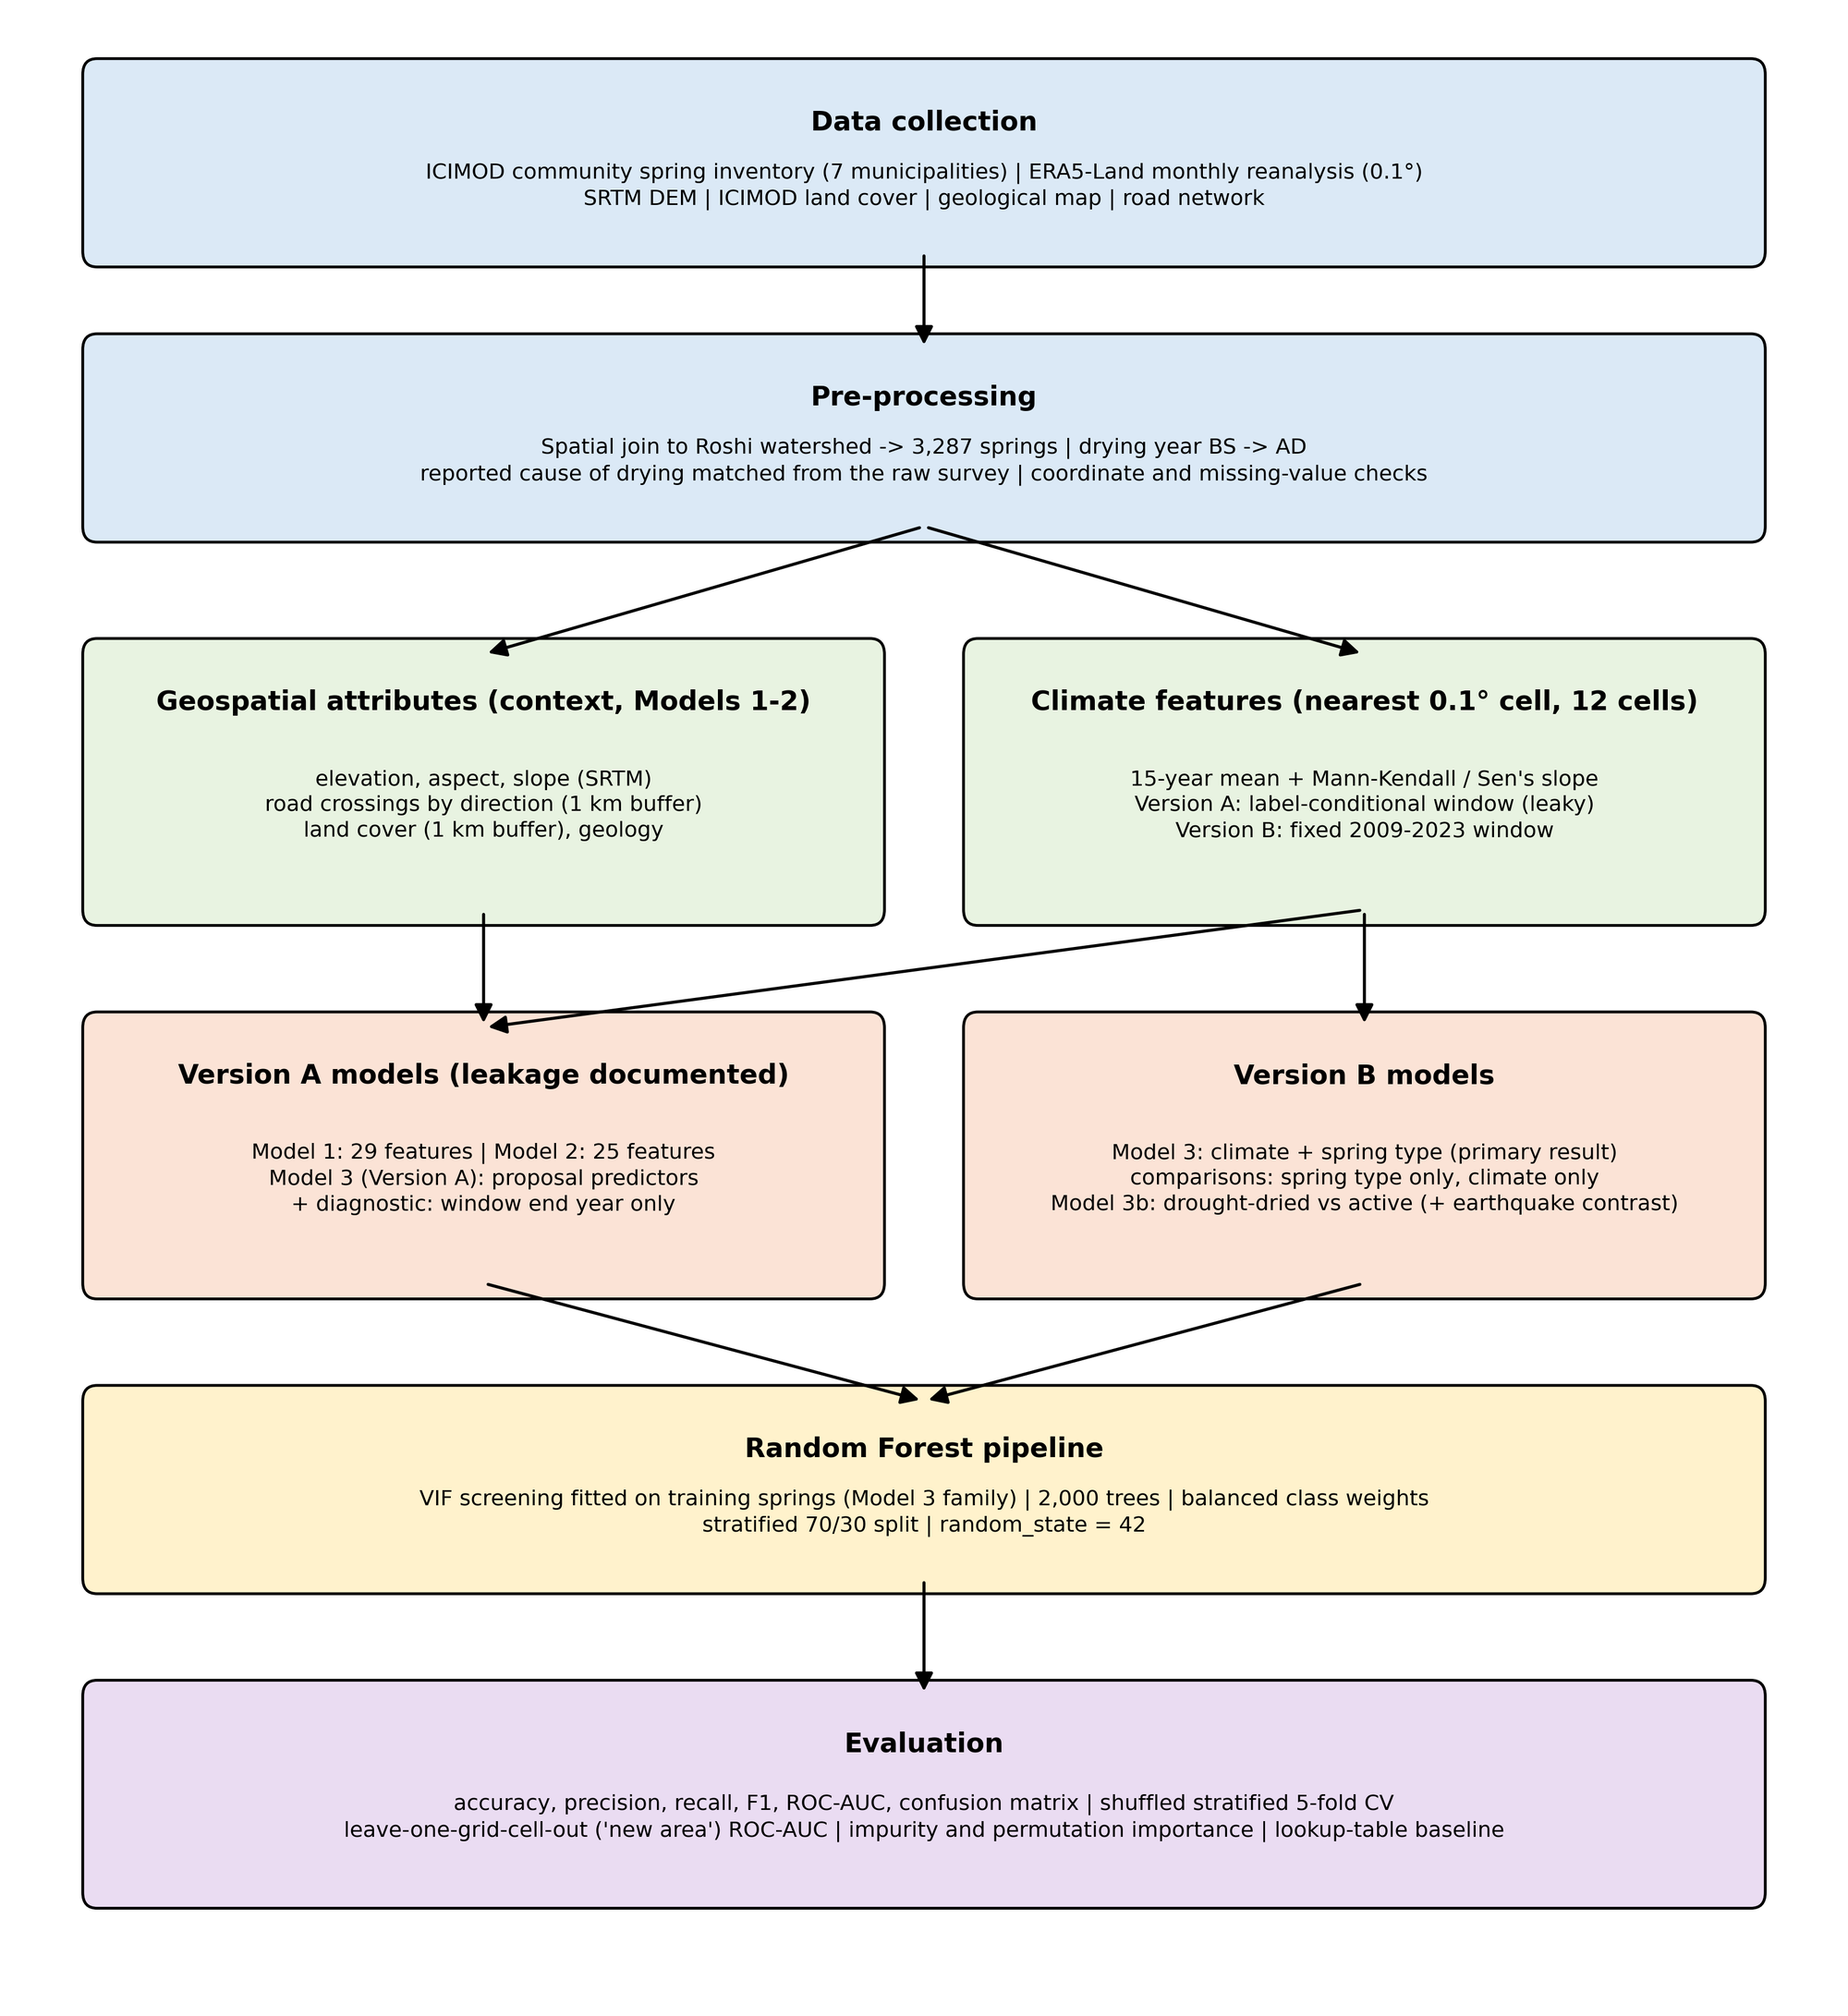
\includegraphics[width=0.8\linewidth]{figures/fig10_methodology_flowchart}
\caption{Methodological workflow of the project.}
\label{fig:flow}
\end{figure}

\clearpage
\section{Model Development and Results}\label{sec:results}

Five model configurations were developed in sequence, plus comparison and sensitivity runs (Table~\ref{tab:design}). Models 1 and 2 were exploratory and progressively narrowed the feature set. Model 3 was built to match the proposal and was first run with the Version A window. The near-perfect scores of these three models led to the leakage diagnosis of Section~\ref{sec:leakage}, after which Model 3 was re-run with the fixed Version B window; that run is the primary result. All results below come from the reproducible notebooks listed in Appendix A.

\subsection{Model 1: exploratory full-feature model}\label{sec:m1}

Model 1 was an initial broad feature-screening model, built before the proposal excluded terrain and roads from the predictor set. It uses 29 predictors: spring type, elevation, aspect in degrees and as eight one-hot classes, eight directional road counts, the two slope terms and the eight Version A climate features, without VIF screening. In the submitted version, every predictor was cast to an integer before training, which truncated the dewpoint, temperature and evaporation trends, the evaporation mean and \texttt{Slope\_\allowbreak{}cos} to zero. That error has been corrected here, so the figures below differ from those submitted.

Model 1 reaches accuracy 0.994, F1 0.986 and ROC-AUC 0.995 on the test set (Table~\ref{tab:versionA}, Figure~\ref{fig:m1cm}), with only 3 active springs misclassified as dried and 3 dried springs missed. Its most important predictors are climate trend features (\texttt{Evaporation\_\allowbreak{}rate} 37.0\%, \texttt{Temperature\_\allowbreak{}rate} 19.1\% of impurity importance; Figure~\ref{fig:m1imp}).

\begin{figure}[htbp]
\centering
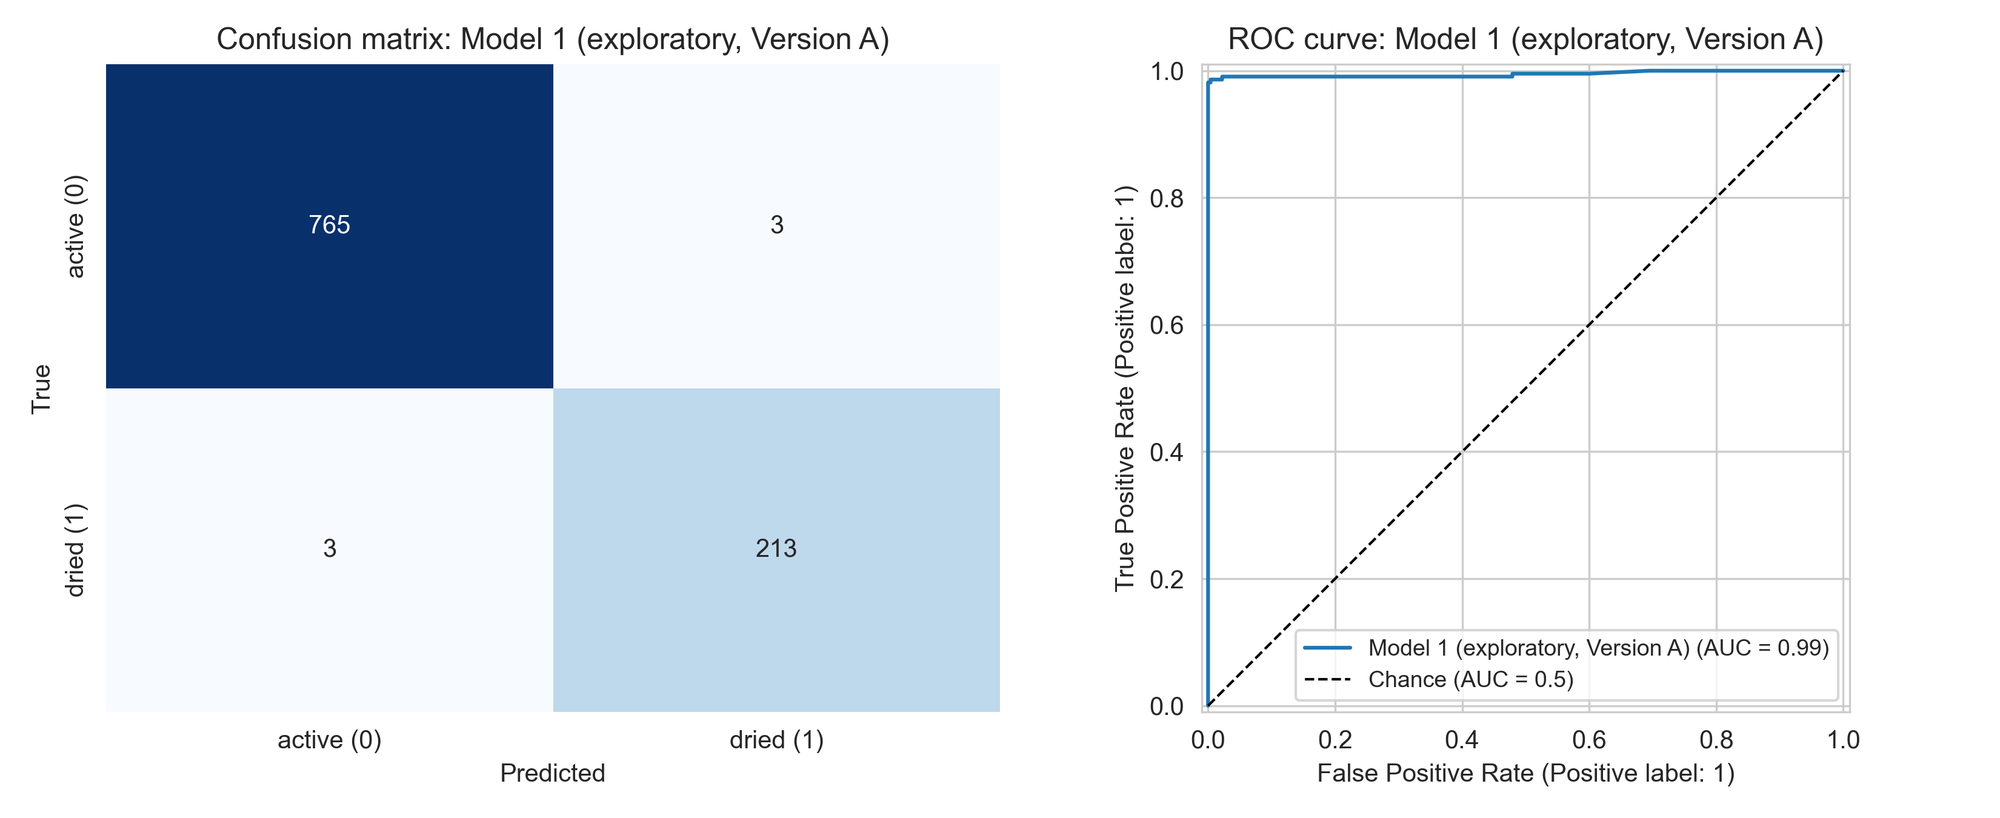
\includegraphics[width=0.95\linewidth]{figures/fig11_model1_exploratory_confusion_roc}
\caption{Model 1: confusion matrix and ROC curve on the held-out test set.}
\label{fig:m1cm}
\end{figure}

\begin{figure}[htbp]
\centering
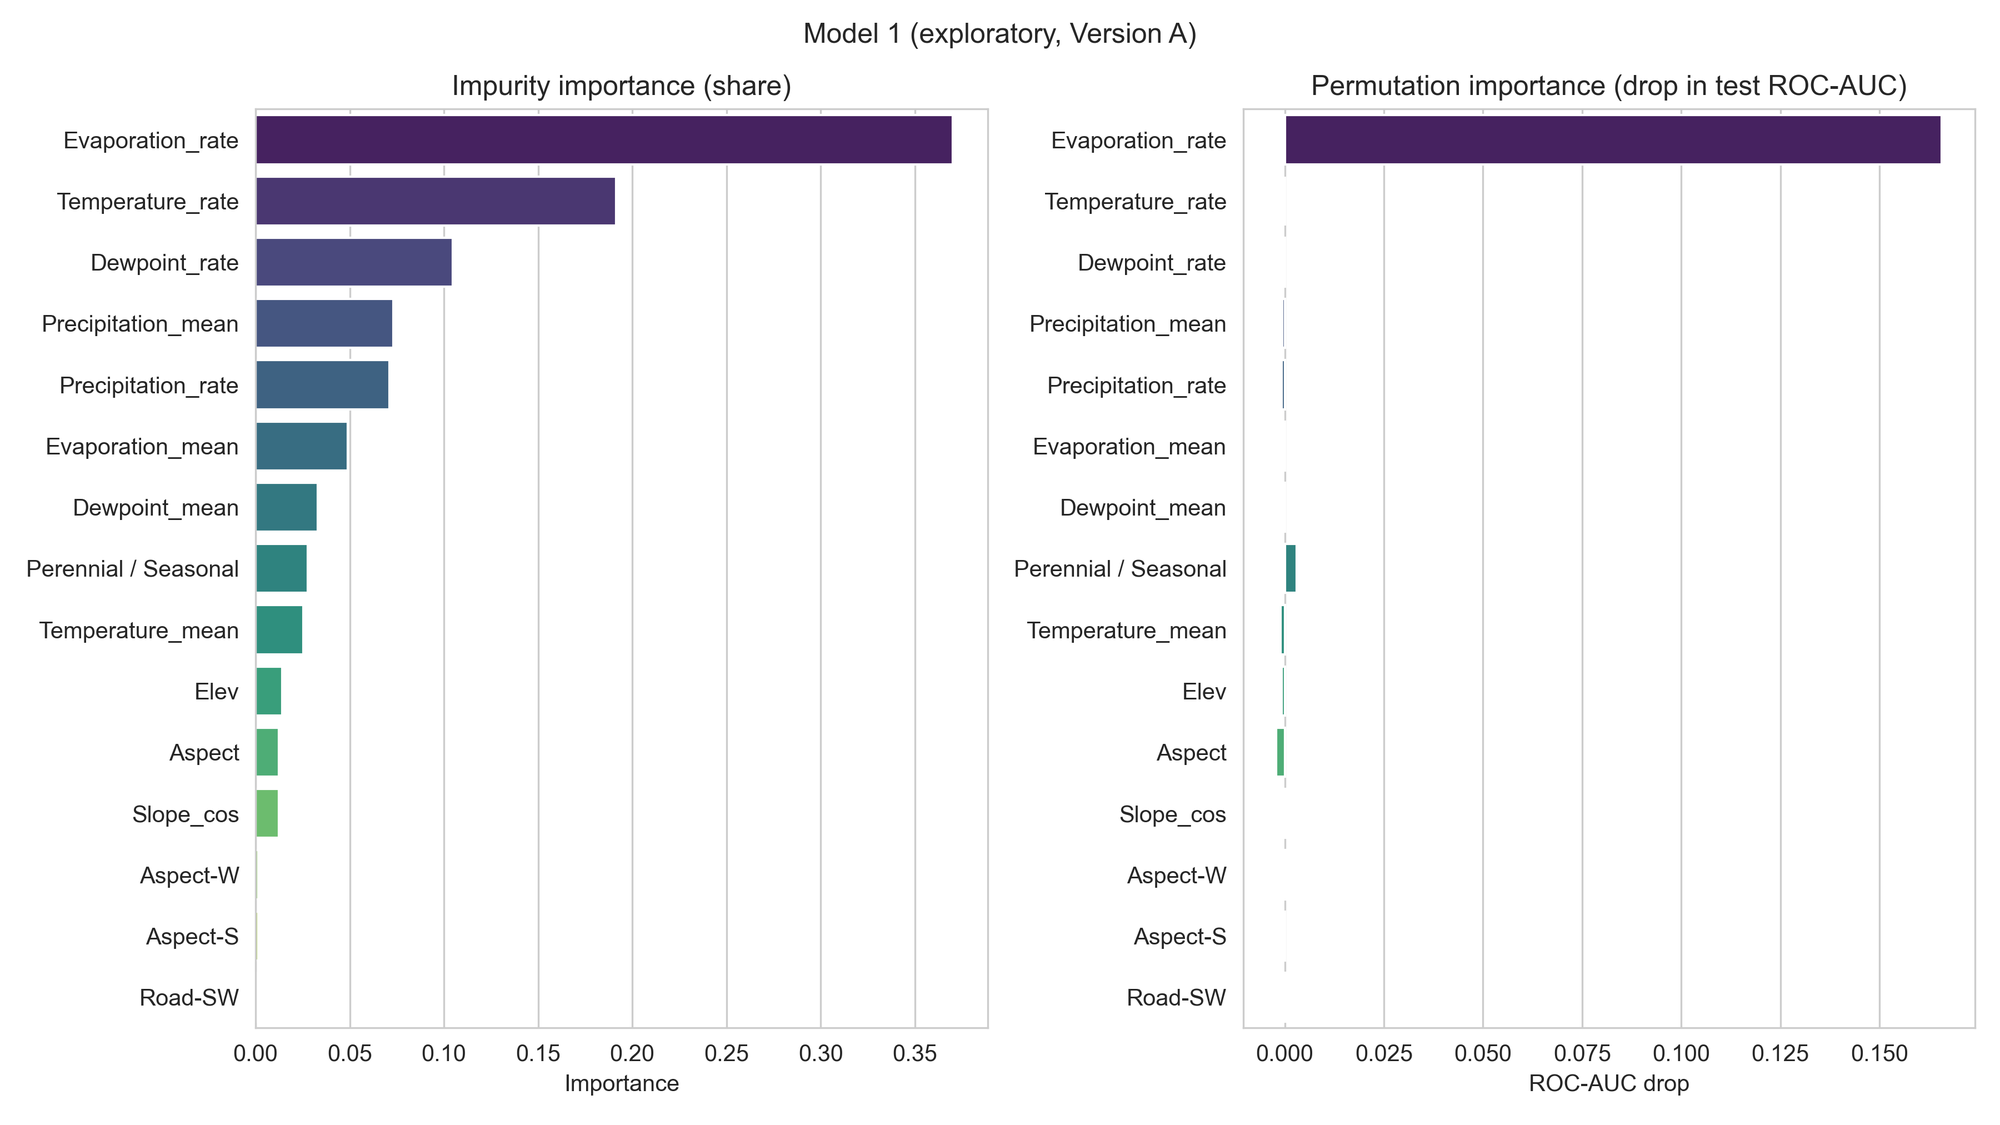
\includegraphics[width=0.95\linewidth]{figures/fig12_model1_exploratory_feature_importance}
\caption{Model 1: impurity and permutation importance of the 15 most important predictors.}
\label{fig:m1imp}
\end{figure}

\subsection{Model 2: refined feature set}\label{sec:m2}

Model 2 narrowed the feature set of Model 1 towards the variables that could be used in the planned scenario projections. Land cover and geology were not used (land cover cannot be projected consistently with the SSP scenarios and is missing before 2000; the geological map is too coarse), the evaporation mean and trend were removed, and the degenerate slope terms were left out. The submitted version justified removing evaporation by its low importance in Model 1. That low importance was an artefact of the integer casting described above: with the error corrected, \texttt{Evaporation\_\allowbreak{}rate} is the most important predictor of Model 1. The original Model 2 code was not archived, so Model 2 was re-created from its description; it uses 25 predictors.

Model 2 performs almost identically to Model 1 (accuracy 0.990, F1 0.977, ROC-AUC 0.994; Table~\ref{tab:versionA}, Figure~\ref{fig:m2cm}). Its most important predictors are again climate trends (\texttt{Temperature\_\allowbreak{}rate} 32.3\%, \texttt{Dewpoint\_\allowbreak{}rate} 20.0\%; Figure~\ref{fig:m2imp}). In the submitted version, the confusion-matrix figure shown for Model 2 was the same image as that of Model 1.

\begin{figure}[htbp]
\centering
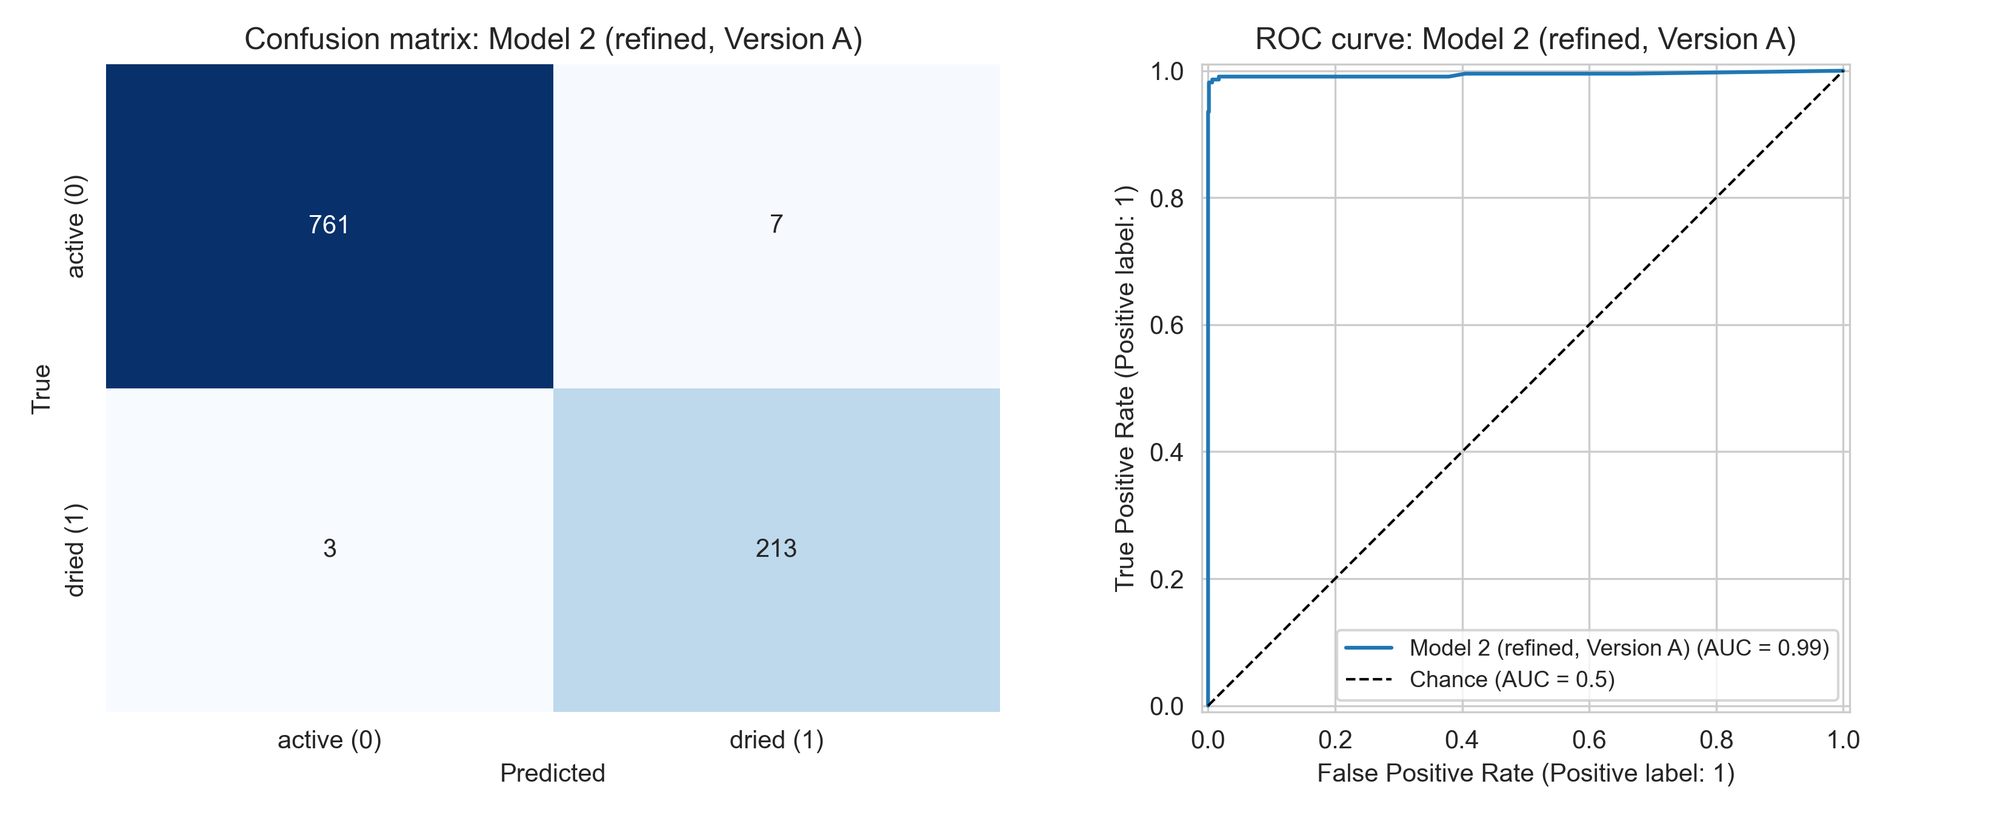
\includegraphics[width=0.95\linewidth]{figures/fig13_model2_refined_confusion_roc}
\caption{Model 2: confusion matrix and ROC curve on the held-out test set.}
\label{fig:m2cm}
\end{figure}

\begin{figure}[htbp]
\centering
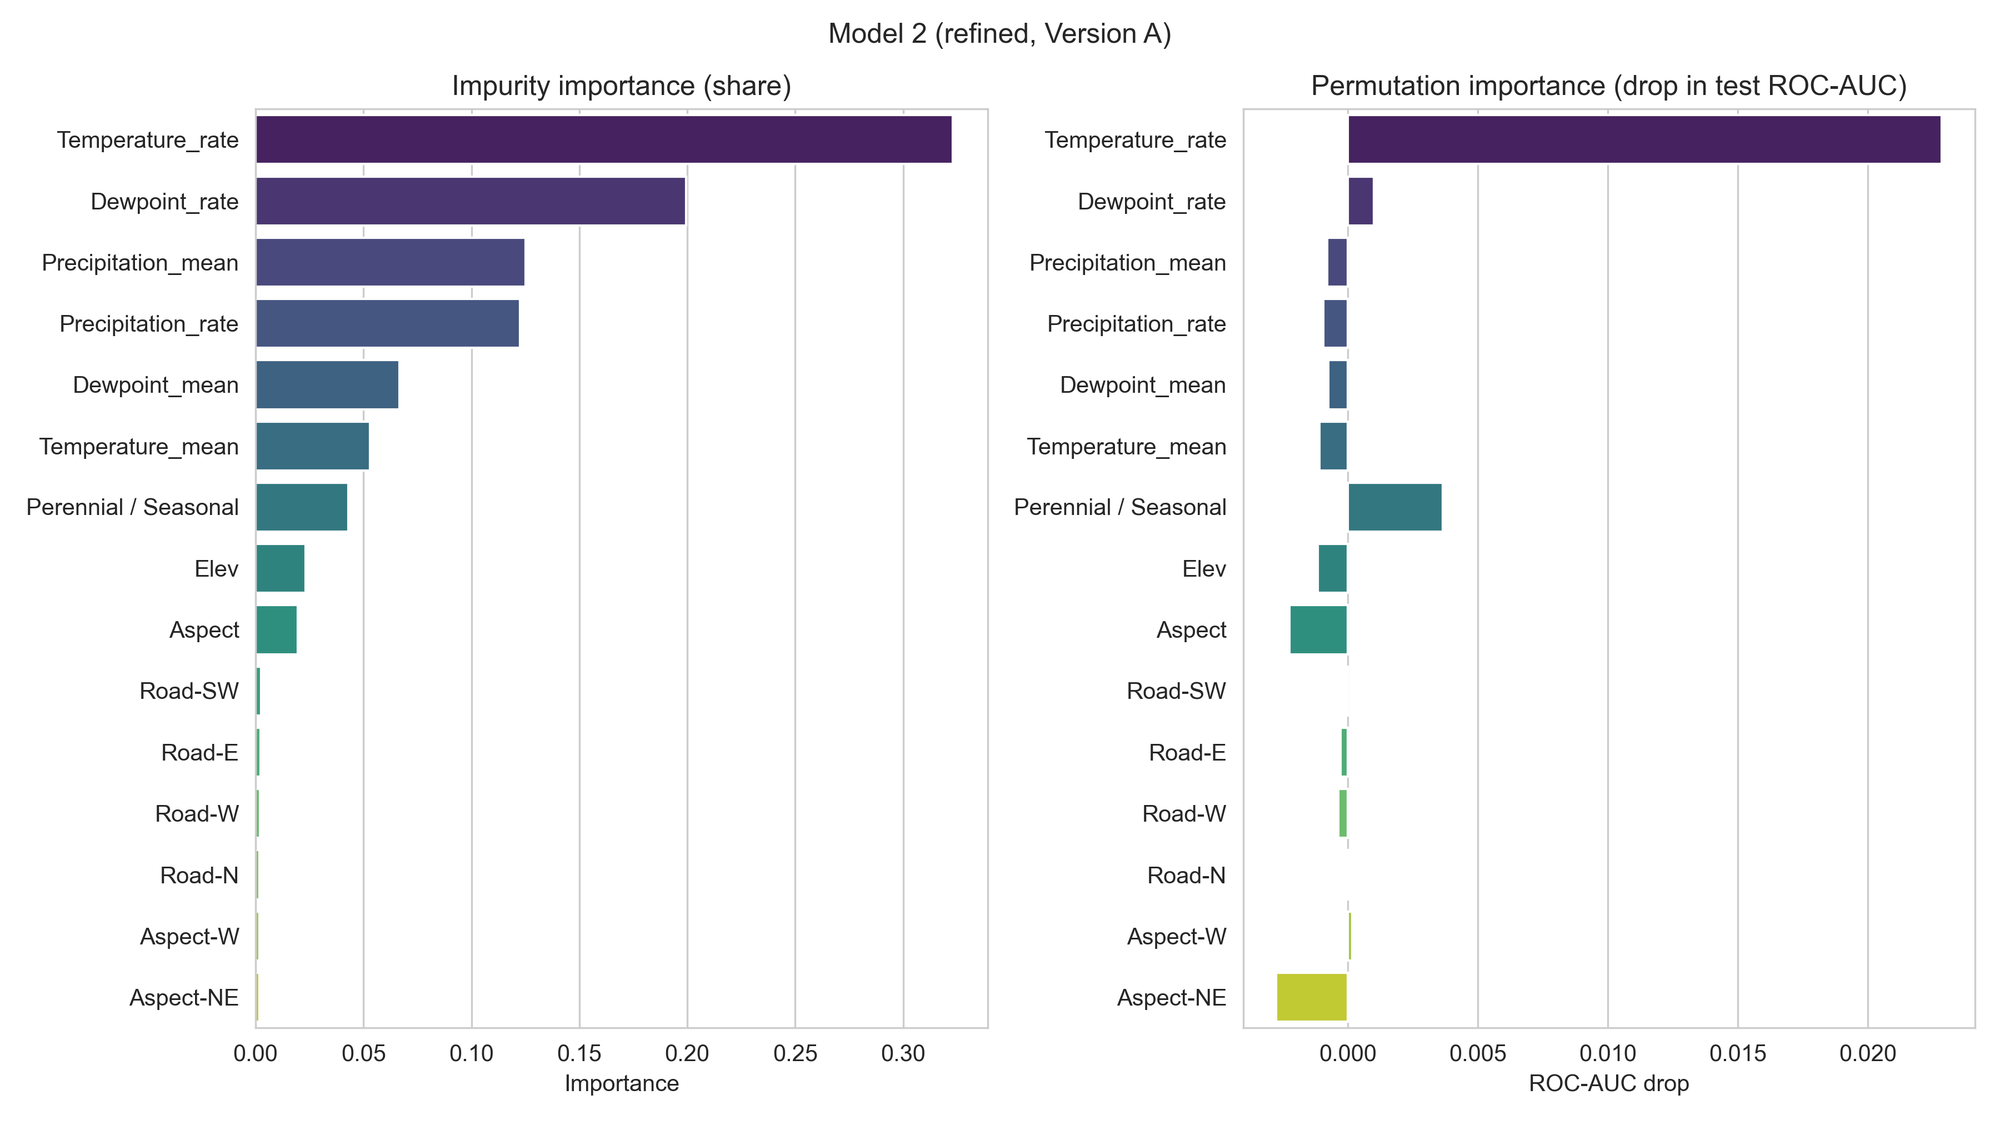
\includegraphics[width=0.95\linewidth]{figures/fig14_model2_refined_feature_importance}
\caption{Model 2: impurity and permutation importance of the 15 most important predictors.}
\label{fig:m2imp}
\end{figure}

\subsection{Model 3 with the Version A window}\label{sec:m3va}

Model 3 implements the proposal's predictor set: the eight climate features and spring type, with VIF screening. With the Version A window, the screening removed \texttt{Dewpoint\_\allowbreak{}mean} (VIF 50.2) and the model reached accuracy 0.983, F1 0.962 and ROC-AUC 0.998 (Table~\ref{tab:versionA}, Figure~\ref{fig:m3vacm}), with \texttt{Evaporation\_\allowbreak{}rate} (41.3\%) and \texttt{Temperature\_\allowbreak{}rate} (22.9\%) as the leading predictors (Figure~\ref{fig:m3vaimp}). In the submitted version these near-perfect values were attributed to Model 2.

\begin{table}[htbp]
\centering
\small
\caption{Results of the three models built on Version A climate features (test set n = 984, of which 216 dried; cross-validation over 3,278 springs)}
\label{tab:versionA}
\begin{tabularx}{\linewidth}{LRRR}
\toprule
\textbf{Metric} & \textbf{Model 1} & \textbf{Model 2} & \textbf{Model 3 (Version A)} \\
\midrule
Accuracy & 0.994 & 0.990 & 0.983 \\
Precision & 0.986 & 0.968 & 0.938 \\
Recall & 0.986 & 0.986 & 0.986 \\
F1 & 0.986 & 0.977 & 0.962 \\
ROC-AUC & 0.995 & 0.994 & 0.998 \\
5-fold CV F1 (mean $\pm$ sd) & 0.985 $\pm$ 0.006 & 0.983 $\pm$ 0.004 & 0.974 $\pm$ 0.014 \\
5-fold CV ROC-AUC (mean $\pm$ sd) & 0.994 $\pm$ 0.003 & 0.994 $\pm$ 0.004 & 0.992 $\pm$ 0.004 \\
\bottomrule
\end{tabularx}
\end{table}

\begin{figure}[htbp]
\centering
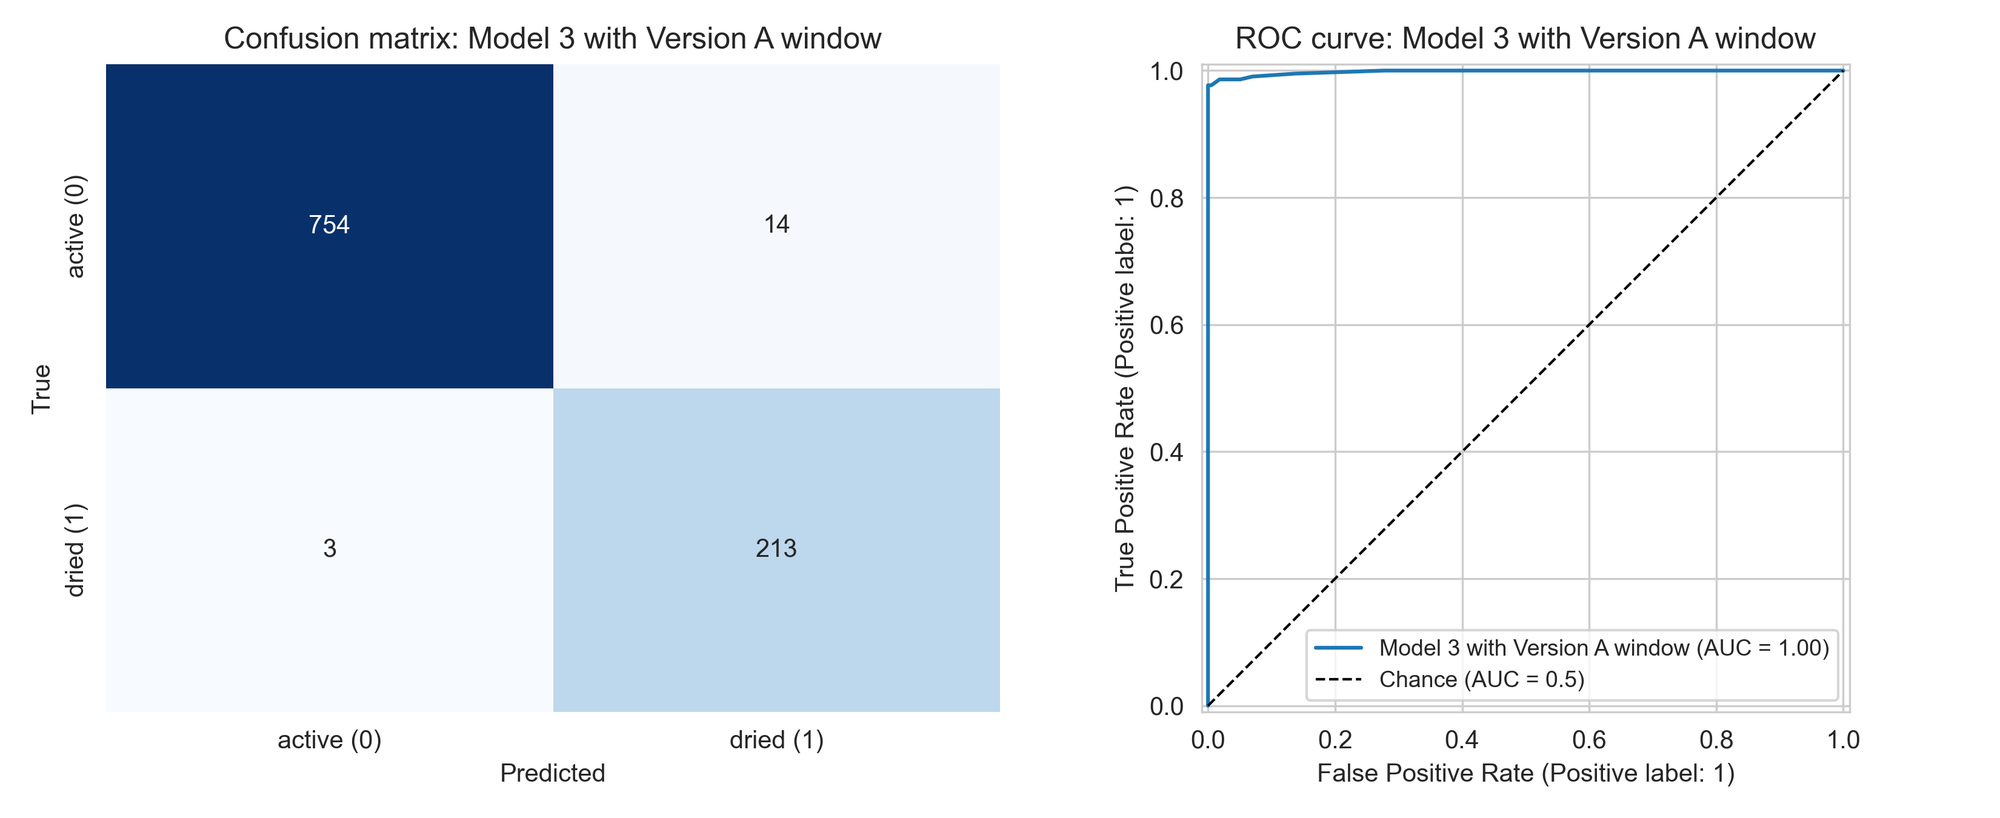
\includegraphics[width=0.95\linewidth]{figures/fig15_model3_version_a_confusion_roc}
\caption{Model 3 with the Version A window: confusion matrix and ROC curve on the held-out test set.}
\label{fig:m3vacm}
\end{figure}

\begin{figure}[htbp]
\centering
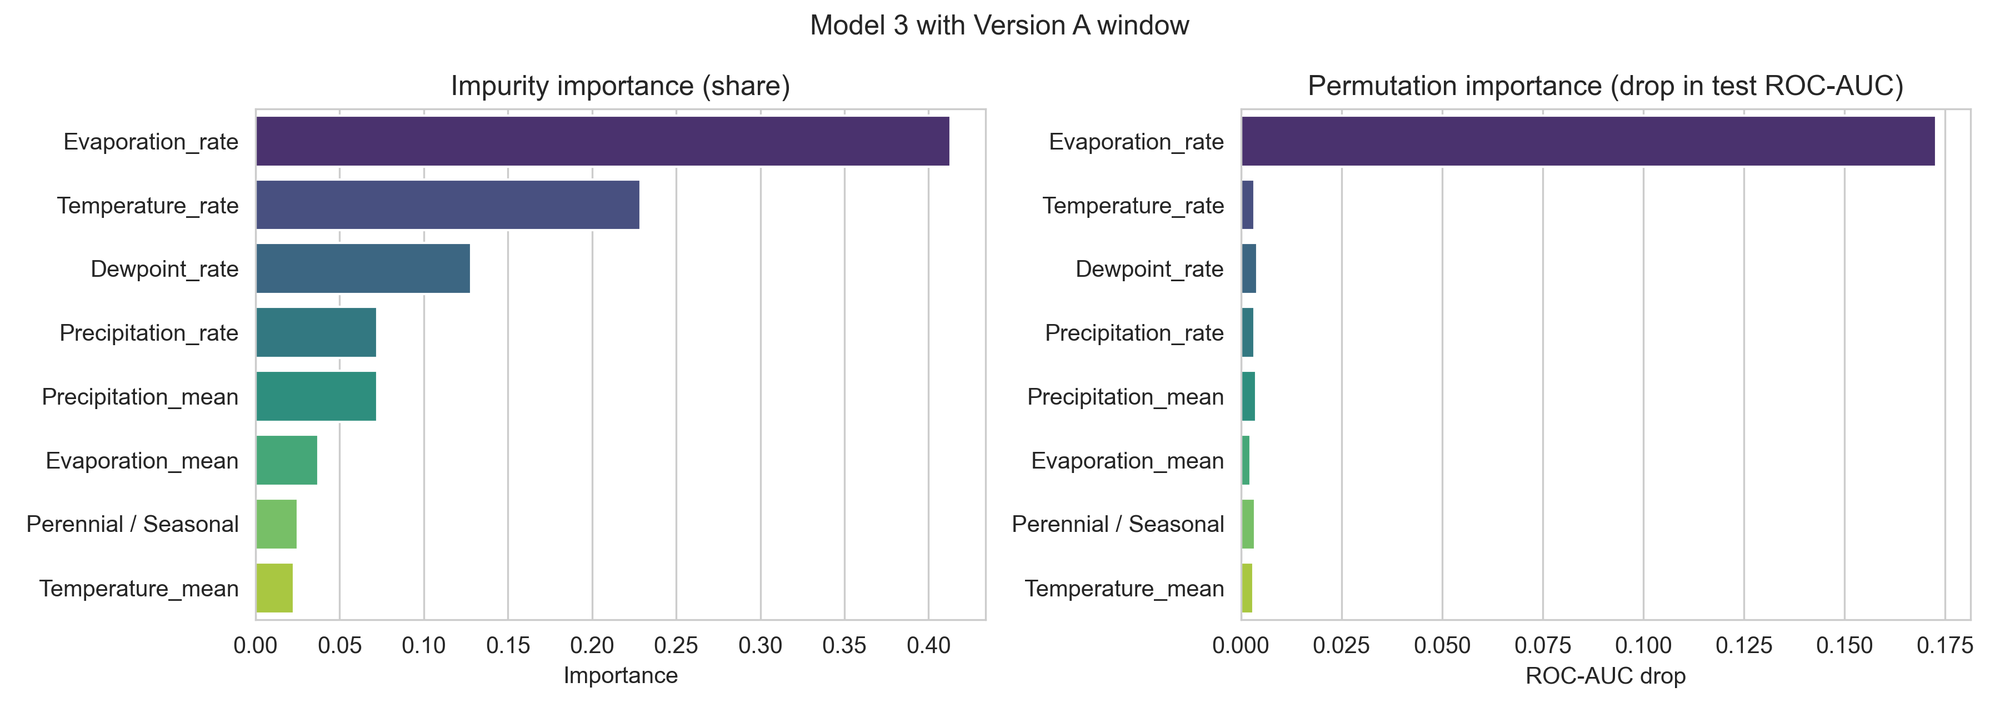
\includegraphics[width=0.95\linewidth]{figures/fig16_model3_version_a_feature_importance}
\caption{Model 3 with the Version A window: impurity and permutation importance.}
\label{fig:m3vaimp}
\end{figure}

\subsection{Discovery of the temporal leakage in the Version A window}\label{sec:leakage}

ROC-AUC values of 0.994 to 0.998 are implausibly high for a real-world hydrological classification task based on regional climate data, and they warranted scrutiny rather than acceptance.

The cause lies in the construction of the Version A window. Every active spring's window ends in the survey year, 2023, whereas a dried spring's window ends in its own drying year, which for most dried springs is earlier (median 2015; only 20 dried springs dried in 2023). The calendar period from which a spring's climate features are drawn is therefore almost mechanically determined by its label. Because regional climate varies from year to year (Figure~\ref{fig:windows}), climate summaries over different periods differ systematically, and the model can learn the period of the window rather than any relationship between climate and spring status. In the terms of \citet{kaufman2011}, the predictors were constructed using information (the drying year) that is only available because the outcome is known, which is target leakage.

A direct diagnostic confirms the explanation. A Random Forest given only one input, the end year of each spring's Version A window, with no climate information at all, classifies the test springs with accuracy 0.994, F1 0.986 and ROC-AUC 0.986. The near-perfect performance of Models 1, 2 and 3 (Version A) is therefore an artefact of predictor construction. The dominance of the trend features fits this explanation, since trends are the features most sensitive to the choice of period. The correction is to give every spring the same window (Version B).

\subsection{Model 3 with the fixed window (primary result)}\label{sec:m3}

With the fixed window (2009 to 2023), the VIF screening on the training springs removed \texttt{Dewpoint\_\allowbreak{}mean} (VIF 938.6) and then \texttt{Evaporation\_\allowbreak{}mean} (VIF 75.6 after the first removal), leaving six climate predictors with VIFs between 1.37 and 9.39 (Table~\ref{tab:vif}). Together with spring type, Model 3 therefore uses \texttt{Dewpoint\_\allowbreak{}rate}, \texttt{Temperature\_\allowbreak{}rate}, \texttt{Precipitation\_\allowbreak{}rate}, \texttt{Evaporation\_\allowbreak{}rate}, \texttt{Temperature\_\allowbreak{}mean}, \texttt{Precipitation\_\allowbreak{}mean} and the perennial/seasonal attribute.

\begin{table}[htbp]
\centering
\small
\caption{VIF of the Version B climate predictors in the Model 3 training data, before screening and after the two removals}
\label{tab:vif}
\begin{tabularx}{\linewidth}{LRR}
\toprule
\textbf{Predictor} & \textbf{Initial VIF} & \textbf{Final VIF} \\
\midrule
Dewpoint\_mean & 938.6 & removed (1st) \\
Temperature\_mean & 884.5 & 5.72 \\
Evaporation\_mean & 77.2 & removed (2nd) \\
Precipitation\_rate & 65.0 & 4.75 \\
Evaporation\_rate & 60.7 & 1.37 \\
Precipitation\_mean & 43.1 & 7.20 \\
Dewpoint\_rate & 21.4 & 9.39 \\
Temperature\_rate & 10.8 & 8.68 \\
\bottomrule
\end{tabularx}
\end{table}

On the held-out test set (987 springs, 218 dried), Model 3 achieved the results in Table~\ref{tab:m3}. In the confusion matrix (Figure~\ref{fig:m3cm}), 584 of 769 active springs are correctly classified and 185 are misclassified as dried, while 126 of 218 dried springs are correctly identified and 92 are missed.

\begin{table}[htbp]
\centering
\small
\caption{Model 3 (fixed window): test-set, cross-validation and new-area results}
\label{tab:m3}
\begin{tabularx}{\linewidth}{LR}
\toprule
\textbf{Measure} & \textbf{Value} \\
\midrule
Accuracy (test) & 0.719 \\
Precision (test) & 0.405 \\
Recall (test) & 0.578 \\
F1 (test) & 0.476 \\
ROC-AUC (test) & 0.748 \\
ROC-AUC (test), 95\% bootstrap CI & 0.710 to 0.783 \\
PR-AUC (test; random ranking = 0.221) & 0.466 \\
PR-AUC (test), 95\% bootstrap CI & 0.404 to 0.533 \\
5-fold CV F1, shuffled (mean $\pm$ sd) & 0.511 $\pm$ 0.023 \\
5-fold CV ROC-AUC, shuffled (mean $\pm$ sd) & 0.760 $\pm$ 0.011 \\
New-area ROC-AUC (leave-one-grid-cell-out) & 0.630 \\
\bottomrule
\end{tabularx}
\end{table}

\begin{figure}[htbp]
\centering
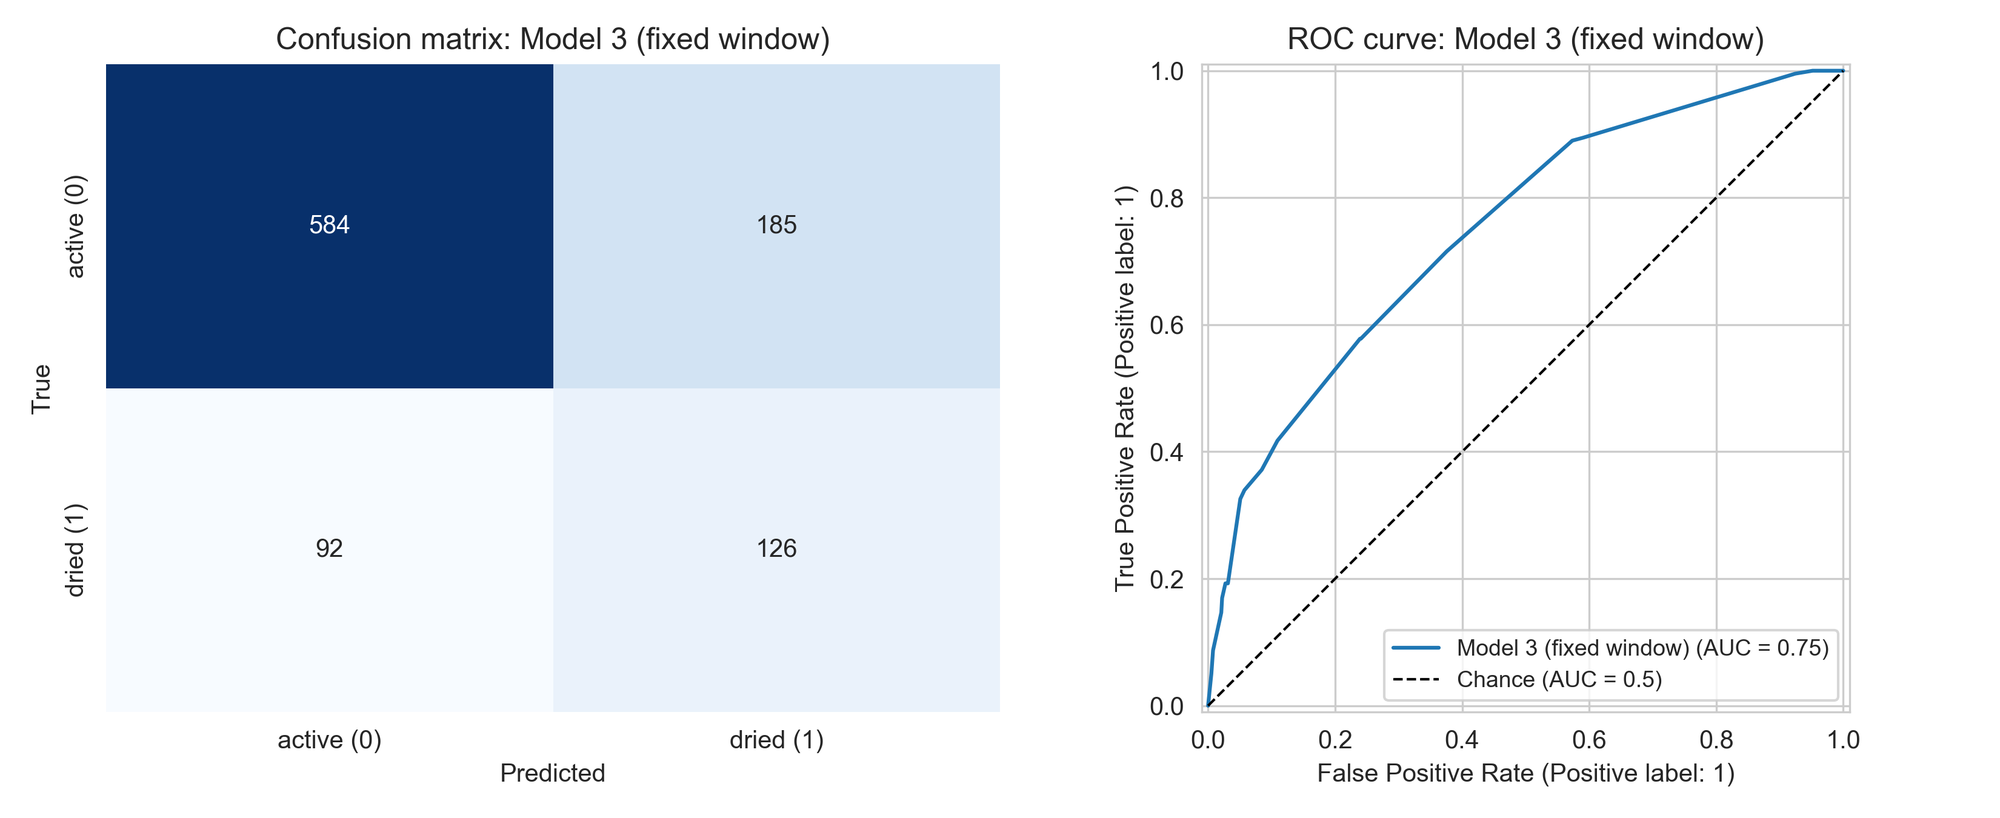
\includegraphics[width=0.95\linewidth]{figures/fig17_model3_final_confusion_roc}
\caption{Model 3 (fixed window): confusion matrix and ROC curve on the held-out test set.}
\label{fig:m3cm}
\end{figure}

\textbf{Cross-validation.} The submitted version reported a 5-fold cross-validated F1 of 0.360 $\pm$ 0.106, obtained with folds taken in file order. The dataset file is ordered: the share of dried springs in its five consecutive fifths is 20.7\%, 19.5\%, 20.4\%, 11.4\%, 38.7\%, so unshuffled folds differ strongly in class balance, and one fold scored F1 0.166. With shuffled stratified folds the cross-validated F1 is 0.511 $\pm$ 0.023, consistent with the test-set value. Most of the apparent instability in the submitted version came from the fold construction rather than from the model.

\subsection{What Model 3 learns}\label{sec:m3-imp}

Perennial/seasonal classification dominates both importance measures (Table~\ref{tab:imp}, Figure~\ref{fig:m3imp}). It accounts for 64.9\% of impurity importance, and shuffling it lowers the test ROC-AUC by 0.164, whereas shuffling any single climate predictor changes the test ROC-AUC by at most 0.003. The climate predictors are strongly redundant with one another, so the loss of one shuffled predictor can be compensated by the others; together they still carry information (see the comparison in Section~\ref{sec:m3b}).

\begin{table}[htbp]
\centering
\small
\caption{Model 3 variable importance}
\label{tab:imp}
\begin{tabularx}{\linewidth}{LRR}
\toprule
\textbf{Predictor} & \textbf{Impurity importance (\%)} & \textbf{Permutation importance (ROC-AUC drop)} \\
\midrule
Perennial / Seasonal & 64.9 & 0.1643 \\
Precipitation\_rate & 8.6 & 0.0033 \\
Temperature\_mean & 7.4 & 0.0028 \\
Temperature\_rate & 6.5 & -0.0010 \\
Precipitation\_mean & 5.0 & -0.0007 \\
Dewpoint\_rate & 3.9 & 0.0013 \\
Evaporation\_rate & 3.6 & -0.0013 \\
\bottomrule
\end{tabularx}
\end{table}

\begin{figure}[htbp]
\centering
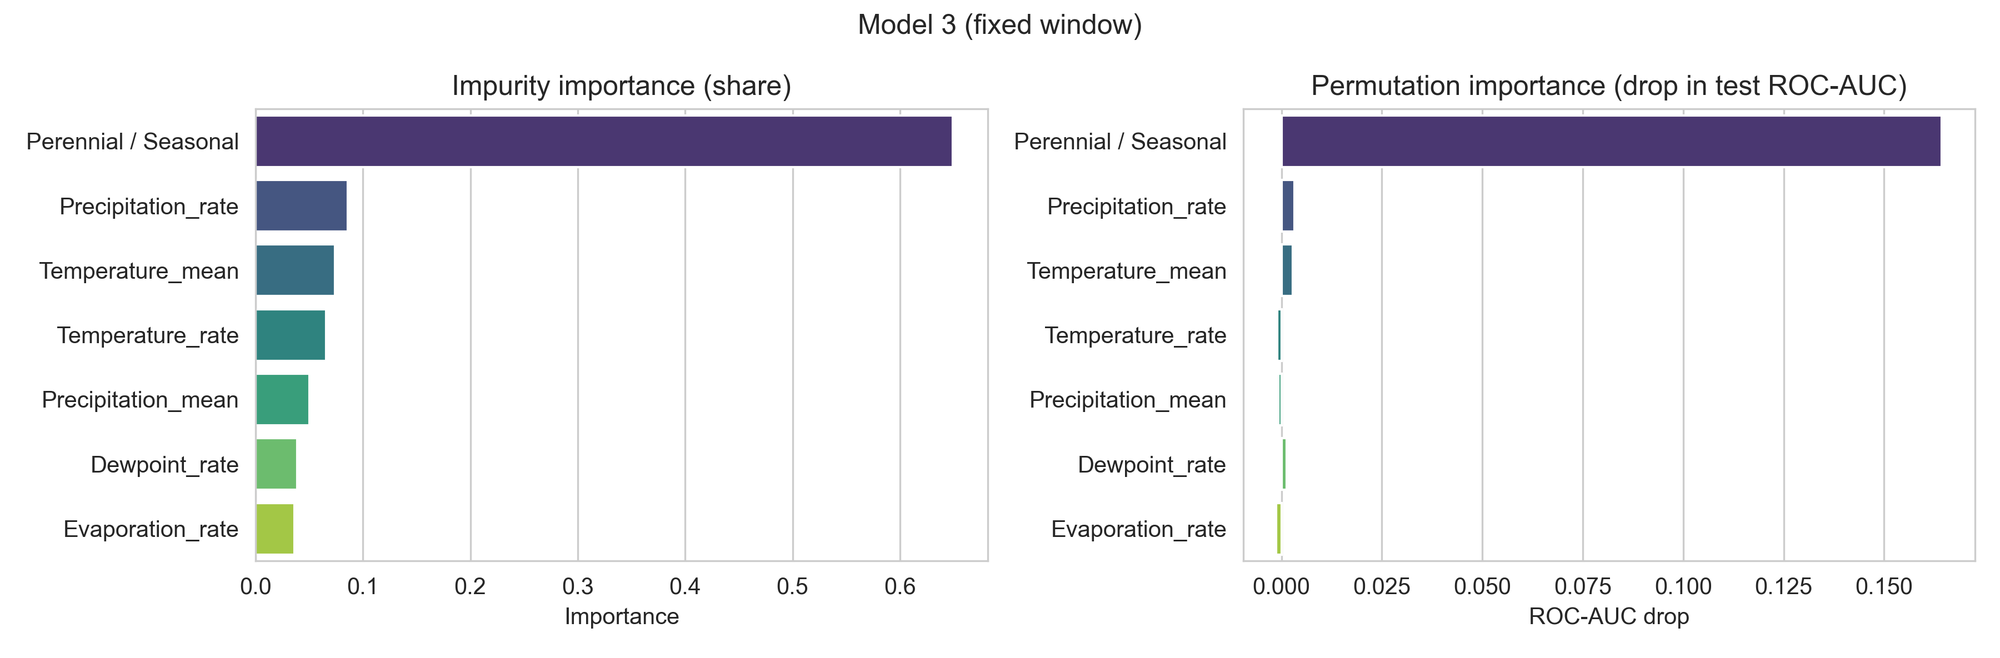
\includegraphics[width=0.95\linewidth]{figures/fig18_model3_final_feature_importance}
\caption{Model 3 (fixed window): impurity and permutation importance.}
\label{fig:m3imp}
\end{figure}

Because all springs in a grid cell share the same climate values, the 3,287 springs have only 23 distinct combinations of predictor values (12 cells $\times$ 2 spring types, where present), and 99.9\% of test springs have an exact counterpart in the training set. A simple lookup table that assigns each test spring the dried share of its predictor combination in the training set reaches a test ROC-AUC of 0.748, the same as the Random Forest (0.748). Model 3 therefore learns the dried rate of each grid cell for perennial and seasonal springs; it cannot distinguish springs within a cell that share a spring type.

\subsection{Input comparison and Model 3b: label screening by drying cause}\label{sec:m3b}

Table~\ref{tab:compare} and Figure~\ref{fig:compare} compare Model 3 with models that use only spring type or only climate, and with models trained on subsets of the dried springs defined by their reported cause. Spring type alone reaches a test ROC-AUC of 0.651 and climate alone 0.625; together (Model 3) they reach 0.748, so each carries information the other does not.

Model 3b repeats Model 3 but keeps only the 226 springs whose drying was attributed to drought or reduced precipitation, compared with all 2,560 active springs. Its test ROC-AUC is 0.854 (95\% CI 0.811 to 0.893; cross-validated 0.862 $\pm$ 0.030), and with climate predictors alone 0.771, compared with 0.625 for climate alone on all dried springs. The contrast model, which keeps only the 229 earthquake-attributed dried springs, reaches 0.709 (95\% CI 0.644 to 0.769). The confidence intervals of Model 3b and Model 3 (0.710 to 0.783) do not overlap, nor do those of Model 3b and the earthquake contrast. Climate predictors therefore separate drought-dried springs from active springs better than they separate earthquake-dried springs. That is the physically expected direction: the climate signal is present but diluted when drying from non-climatic causes is mixed into the dried class.

Model 3b's F1 (0.393) is lower than Model 3's even though its ROC-AUC is higher, because dried springs make up only 8.1\% of its data. With so few positives, the false alarms (161) outnumber the correctly identified dried springs (56 of 68), which lowers precision and F1. Its PR-AUC (0.338) is lower than Model 3's (0.466) for the same reason, but relative to random ranking it is higher: 4.2 times the 0.081 expected by chance, against 2.1 times for Model 3. ROC-AUC does not depend on class prevalence and is the appropriate measure for comparing these configurations (Figure~\ref{fig:m3bcm}).

\begin{table}[htbp]
\centering
\footnotesize
\caption{Comparison of input sets and label screening by reported cause (test set: stratified 30\%; CV: shuffled 5-fold; new area: leave-one-grid-cell-out)}
\label{tab:compare}
\begin{tabularx}{\linewidth}{LRRRRRR}
\toprule
\textbf{Configuration} & \textbf{Springs (dried)} & \textbf{Test F1} & \textbf{Test ROC-AUC} & \textbf{CV F1} & \textbf{CV ROC-AUC} & \textbf{New-area ROC-AUC} \\
\midrule
Spring type only & 3,287 (727) & 0.459 & 0.651 & 0.480 & 0.662 & 0.584 \\
Climate only & 3,287 (727) & 0.370 & 0.625 & 0.401 & 0.637 & 0.527 \\
\textbf{Model 3} (climate + type) & 3,287 (727) & 0.476 & 0.748 & 0.511 & 0.760 & 0.630 \\
\textbf{Model 3b}: drought-dried vs active & 2,786 (226) & 0.393 & 0.854 & 0.391 & 0.862 & 0.752 \\
Model 3b, climate only & 2,786 (226) & 0.283 & 0.771 & 0.292 & 0.768 & 0.543 \\
Earthquake-dried vs active & 2,789 (229) & 0.229 & 0.709 & 0.214 & 0.704 & 0.571 \\
\bottomrule
\end{tabularx}
\end{table}

\begin{figure}[htbp]
\centering
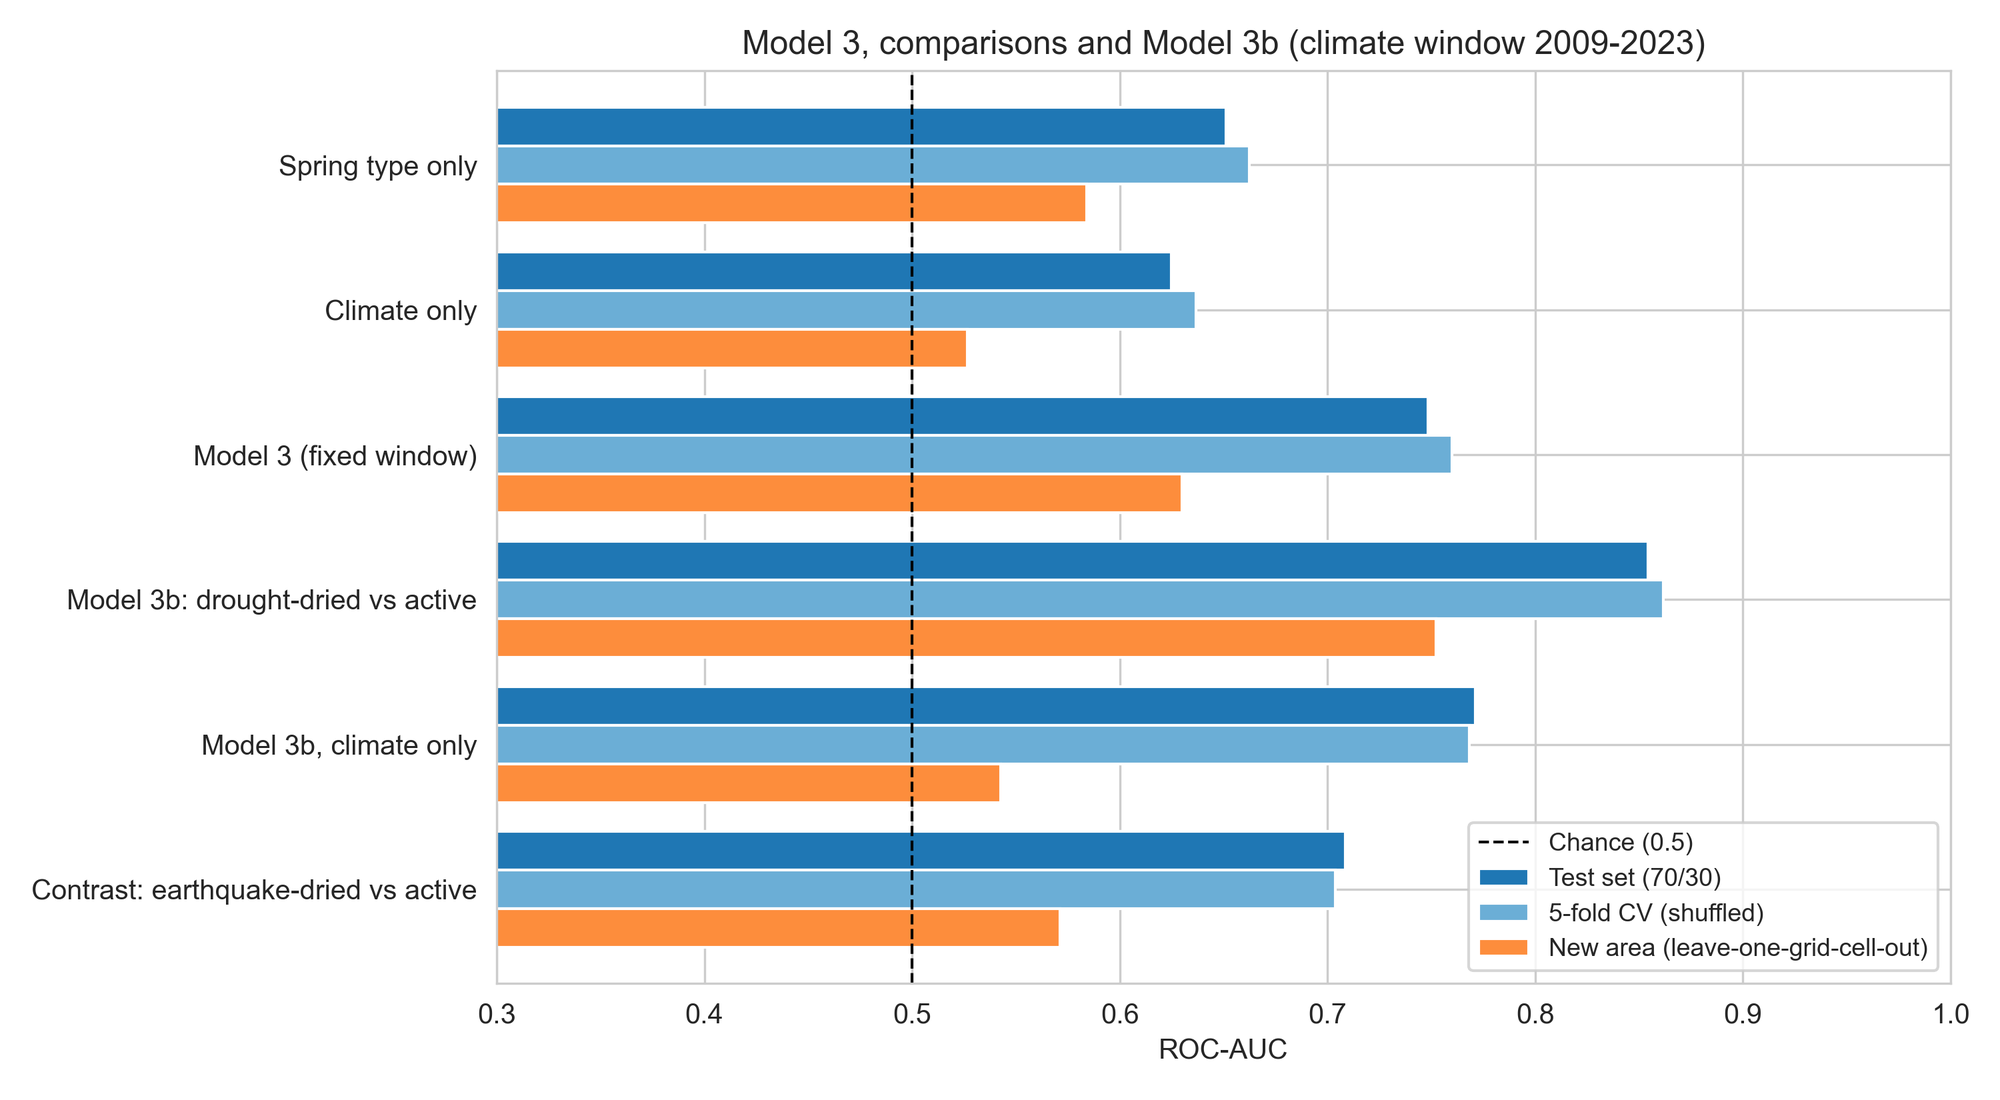
\includegraphics[width=0.95\linewidth]{figures/fig19_model3_comparison}
\caption{ROC-AUC of Model 3, the input comparisons and Model 3b on the test set, in shuffled 5-fold cross-validation and in the new-area (leave-one-grid-cell-out) test.}
\label{fig:compare}
\end{figure}

\begin{figure}[htbp]
\centering
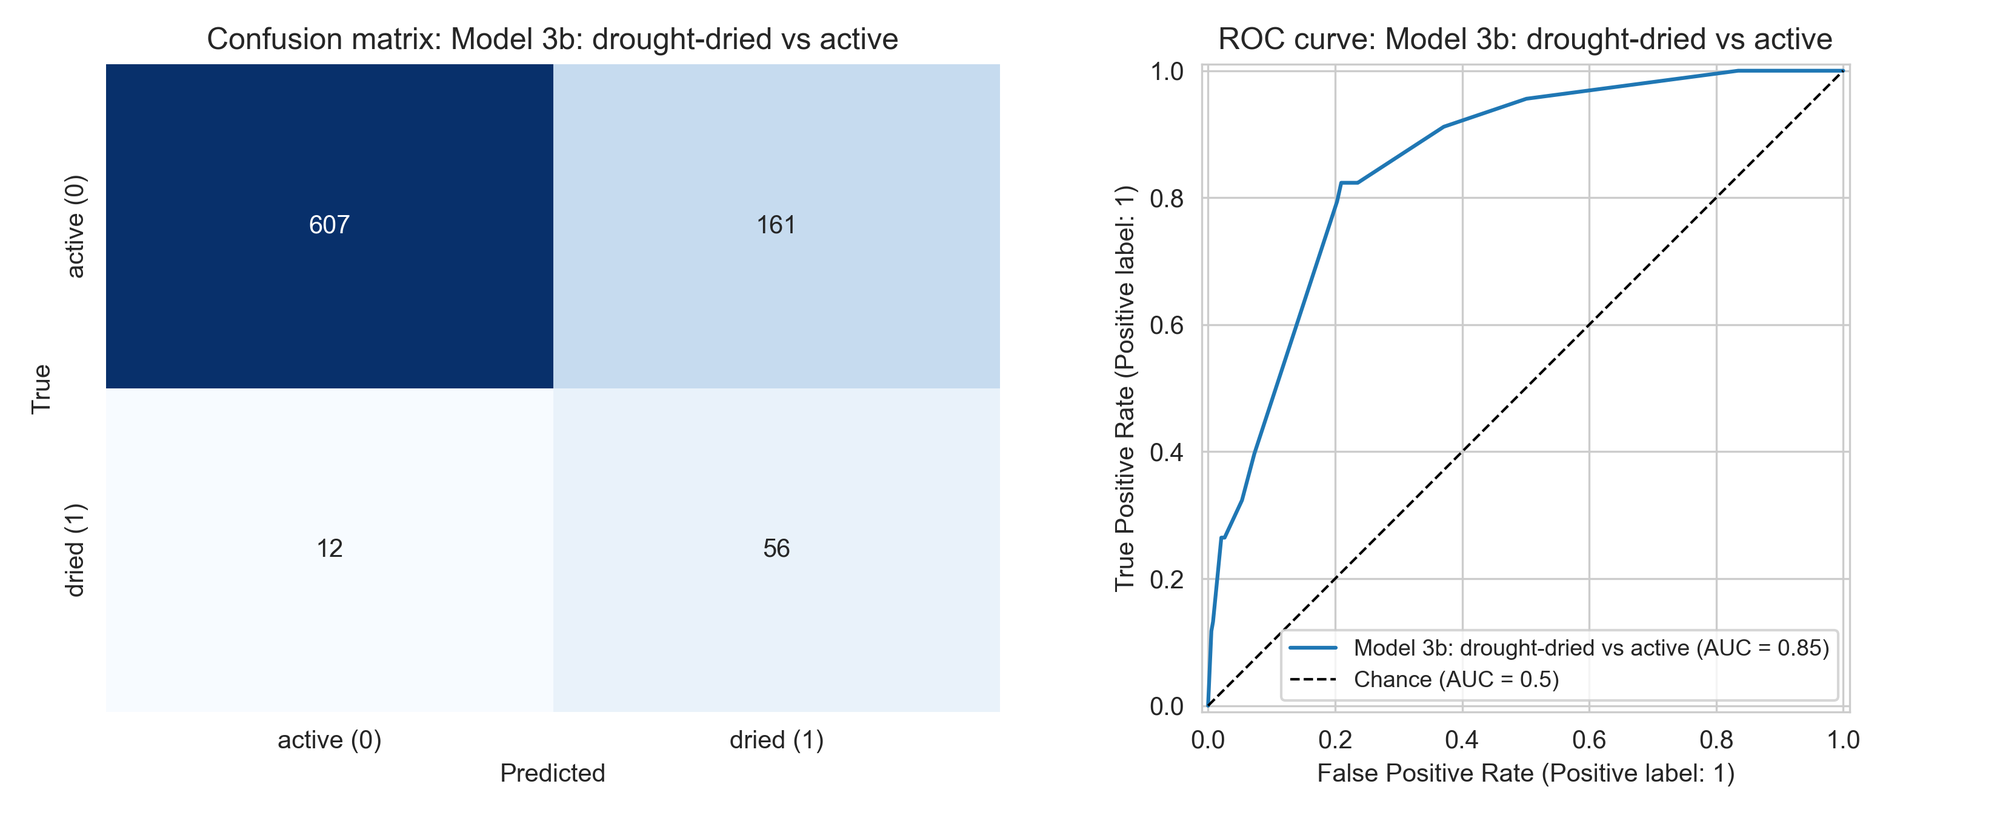
\includegraphics[width=0.95\linewidth]{figures/fig20_model3b_drought_confusion_roc}
\caption{Model 3b (drought-dried vs active springs): confusion matrix and ROC curve on the held-out test set.}
\label{fig:m3bcm}
\end{figure}

\subsection{Performance in unseen areas}\label{sec:newarea}

When whole grid cells are held out, performance falls for every configuration (Table~\ref{tab:compare}, orange bars in Figure~\ref{fig:compare}). Model 3 reaches a new-area ROC-AUC of 0.630, compared with 0.748 on the random test split, and climate alone falls to 0.527, close to random ranking. Model 3b keeps a new-area ROC-AUC of 0.752, but with climate predictors alone it falls to 0.543, so in unseen areas its skill comes mainly from spring type. With only 12 distinct climate locations, the climate predictors identify which cell a spring is in, and a model trained on the other cells has no basis to rank the springs of a new cell by climate. It is the main limitation of the current climate inputs (Section~\ref{sec:limits}).

\clearpage
\section{Discussion}\label{sec:discussion}

\subsection{Descriptive spatial, terrain and infrastructure findings}

Springs in the Roshi Khola watershed are concentrated at mid-elevations. The share of dried springs decreases with elevation and is lower on east- and north-east-facing slopes than on south-, south-west- and west-facing slopes (Section~\ref{sec:topo}), a pattern consistent with the influence of solar radiation and evaporative demand on moisture retention \citep{gutierrez2013,broxton2009}. Dried springs also have more road crossings within 1 km in seven of eight directions, consistent with the capacity of road construction to intercept shallow groundwater and redirect runoff \citep{montgomery1994,dutton2005}. These are descriptive associations: elevation, aspect, roads and climate are correlated across the watershed, and none of these patterns is evidence of an independent or causal effect.

\subsection{Interpretation of model performance}\label{sec:interpret}

The corrected model predicts spring status better than chance, with a test ROC-AUC of 0.748 and a cross-validated ROC-AUC of 0.760 $\pm$ 0.011, against 0.5 for random ranking. The result gives modest support to the within-watershed part of the working hypothesis, and the support is limited for three reasons. First, the perennial/seasonal attribute carries most of the signal. That is physically expected, because seasonal springs are more susceptible to running dry, but it also means that climate adds comparatively little once spring type is known. Second, the climate predictors take only 12 distinct values and act as a location identifier; Model 3 is equivalent to a lookup table of the dried rate per grid cell and spring type (Section~\ref{sec:m3-imp}). Third, performance drops in unseen grid cells (Section~\ref{sec:newarea}). Climate variables and spring type thus contain a moderate within-watershed signal, but the model does not establish a causal climate effect and is not suitable for high-confidence operational use.

The label-screening result qualifies this reading. The climate signal is clearer when only drought-dried springs are compared with active springs (Model 3b), and weaker for earthquake-dried springs. In this inventory 229 of 727 dried springs (31.5\%) are attributed to the earthquake, and most of them dried in 2015. The pattern agrees with the immediate drying effect of the 2015 earthquake reported in the Melamchi area \citep{chapagain2019} and with the multiple causes perceived by local governments \citep{thapa2023}. A climate-driven model of spring drying should therefore be trained on labels that reflect climate-related drying.

\subsection{Comparison with the literature}\label{sec:compare-lit}

Published results are useful here only as broad plausibility references, because prediction targets, predictors, sampling units and validation designs differ (Table~\ref{tab:literature}). The test ROC-AUC of Model 3 (0.748) is of the same order as held-out values reported for related Random Forest tasks, such as 0.748 for water-spring potential in Jordan \citep{alshabeeb2023} and 0.757 for a Random Forest groundwater-potential model without climate factors \citep{guo2023}. It is above the prediction-rate AUC of 0.60 for frequency-ratio groundwater-potential mapping in Shivapuri, Nepal \citep{upadhyaya2024}. The submitted version compared Model 3 with the range of 0.65 to 0.80 from that study, but those values are success-rate AUCs computed on the mapping data. The closest analogue, active-versus-depleted classification of mapped springs in Mongolia \citep{ishikawa2025}, reported ROC-AUC values of 0.84 to 0.86 with satellite and terrain predictors. \citet{niraula2021} found that accuracy fell from 92\% to 75\% on an independent dataset, which parallels the drop observed here in unseen grid cells. The near-perfect values of the Version A models did not pass this plausibility check, which was one reason for the leakage investigation.

\begin{table}[htbp]
\centering
\footnotesize
\caption{Published performance of related tasks (values from the cited abstracts)}
\label{tab:literature}
\begin{tabularx}{\linewidth}{LLLL}
\toprule
\textbf{Study} & \textbf{Task and data} & \textbf{Validation} & \textbf{Reported performance} \\
\midrule
\citet{alshabeeb2023} & Water-spring potential, Jordan; 200 springs, 13 predictors & 70/30 split & ROC-AUC: RF 0.748, SVM 0.732, MARS 0.727, BRT 0.689 \\
\citet{guo2023} & Groundwater potential (productive wells), Yinchuan Plain & held-out data & ROC-AUC: RF 0.757 without climate factors; climate factors +0.073 \\
\citet{upadhyaya2024} & Groundwater potential, Shivapuri RM, Nepal; frequency ratio & success vs prediction rate & success-rate AUC 0.65 (FR), 0.80 (MFR); prediction-rate AUC 0.60 (both) \\
\citet{niraula2021} & Spring occurrence, Central Himalaya; 621 springs, 815 non-springs & 80/20 split; independent dataset & accuracy 92\% (Bootstrap Forest); 75\% on independent data \\
\citet{ishikawa2025} & Discharging vs depleted springs, Mongolia; 228 labelled springs & cross-validation & ROC-AUC 0.84 (LR), 0.86 (RF), 0.84 (SVM) \\
This project, Model 3 & Active vs dried springs, Roshi Khola; 3,287 springs & 70/30 split; 5-fold CV; new area & ROC-AUC 0.748 (test), 0.760 (CV), 0.630 (new area) \\
\bottomrule
\end{tabularx}
\end{table}

\subsection{Class imbalance and dried-spring recall}

Model 3 recovers 126 of 218 dried springs in the test set (recall 0.578) while producing 185 false positives among 769 active springs. The relatively low precision for the dried class reflects both the difficulty of the task and the imbalance of the data (22.1\% dried). Of the 727 dried springs, 218 (30\%) are in the stratified test set. As Model 3b shows, F1 and precision fall further when the positive class becomes rarer, even if ranking improves. ROC-AUC is used to compare configurations for that reason. The precision-recall view \citep{saito2015} gives the same picture: Model 3's PR-AUC of 0.466 (95\% CI 0.404 to 0.533) is about 2.1 times the 0.221 of random ranking, a clear but modest gain.

\subsection{Limitations}\label{sec:limits}

\begin{itemize}
  \item \textbf{Coarse climate inputs.} All springs fall in 12 ERA5-Land cells, so climate values do not vary within a cell; the new-area ROC-AUC (0.630) is the more realistic estimate of performance at unseen locations. Reanalysis precipitation in mountain terrain is also biased \citep{khadka2022,lavers2022}.
  \item \textbf{Label quality.} Spring status comes from a single survey and community reports. Drying years and causes are recalled, a few drying years are inconsistent between calendars, and the persistence of drying is not verified.
  \item \textbf{Non-climatic drying.} About 31\% of dried springs are attributed to the 2015 earthquake and others to infrastructure, neglect or other causes; including them in the dried class dilutes the climate signal.
  \item \textbf{Spring type.} The perennial/seasonal attribute dominates the model. If dried springs were more likely to be recorded as seasonal, part of its importance could reflect the outcome itself; the survey protocol should be checked.
  \item \textbf{Random-split evaluation.} The test set and cross-validation use random splits, so they describe performance for springs in already-sampled cells. Duplicate springs across the split do not change the test ROC-AUC (0.748 without them), but the bootstrap intervals cover only test-set sampling, not the choice of split or of grid cells.
  \item \textbf{Single algorithm and no tuning.} Only Random Forest with fixed settings was evaluated; algorithm comparison is planned for the dissertation.
\end{itemize}

\clearpage
\section{Future Work}\label{sec:future}

\subsection{Label screening by cause and persistence}

The proposal specifies screening dried labels by how long a spring has been dry, and this report adds screening by the reported cause of drying (Model 3b). The dissertation will combine both: define climate-relevant drying labels (drought or reduced precipitation), treat earthquake- and infrastructure-related drying separately, determine an empirical minimum drying duration, and report results with and without low-confidence labels.

\subsection{From one row per spring to a year-by-year design}\label{sec:augmentation}

The submitted version proposed a temporal augmentation in which each active spring contributes one row per year for 2015 to 2023 and each dried spring one row per year from its drying year to 2023, each with the 15-year window ending in that year. Computed on this dataset, that design would produce 23,040 active and 8,795 dried rows, raising the dried share only from 22.1\% to 27.6\%. It would also reintroduce leakage: 3,021 dried rows (34.3\%) fall in years before 2015, for which no active rows exist, so the row year would again predict the label. Rows for years after drying would also describe climate after the spring had already dried, which cannot explain its drying.

A more defensible use of the drying year is a discrete-time, year-by-year design. Each spring contributes one row per year while it is still flowing, labelled 1 in the year it dries and 0 otherwise, and leaves the data after drying; active springs contribute rows labelled 0 up to the survey year. Predictors are the climate conditions preceding each year (for example, rainfall and temperature anomalies over the previous one to three years). The design asks whether springs dry after dry or hot years, uses the large year-to-year variation in climate rather than the small differences between grid cells, and avoids both leakage problems. All rows of a spring, and preferably of a grid cell, must be kept in the same cross-validation fold \citep{roberts2017,john2025}.

\subsection{Finer climate inputs}

Spring-to-spring climate variation can be introduced by adjusting temperature to each spring's elevation using the DEM, by using higher-resolution precipitation products, and by station-based bias correction of reanalysis values, given the known weaknesses of reanalysis precipitation in Himalayan terrain \citep{khadka2022,lavers2022}.

\subsection{Algorithm comparison}

The dissertation will compare Random Forest with logistic regression, gradient boosting such as XGBoost \citep{chen2016}, support vector machines and, if justified by the predictor set, neural networks, with SMOTE or class weighting applied within training folds only \citep{santos2018}. Such a comparison is only informative once the climate inputs vary at the spring scale; with the current 23 distinct predictor combinations, all algorithms reduce to the same lookup table.

\subsection{Staged generalisability testing}

The 2,056 springs outside the analysis dataset remain untouched for staged transfer tests, first in Panchkhal (near domain) and then in the remaining municipalities \citep{wenger2012}. Many of them lie in climate cells already used by Roshi springs (Table~\ref{tab:outside}): only 37.3\% of Panchkhal's 837 springs fall in cells not used in training, and Panchkhal has a much higher dried share (38.9\%) than Roshi (22.1\%). Transfer results should therefore be reported separately for springs in new cells, and the difference in prevalence should be considered when interpreting precision and F1.

\begin{table}[htbp]
\centering
\footnotesize
\caption{Springs outside the analysis dataset by municipality (inventory records not among the 3,287 analysis springs)}
\label{tab:outside}
\begin{tabularx}{\linewidth}{LRRRR}
\toprule
\textbf{Municipality} & \textbf{Springs} & \textbf{ERA5-Land cells} & \textbf{Springs in cells unused by Roshi springs (\%)} & \textbf{Dried (\%)} \\
\midrule
Panchkhal & 837 & 4 & 37.3 & 38.9 \\
Dhulikhel & 596 & 5 & 22.1 & 20.6 \\
Temal & 497 & 5 & 0.2 & 32.6 \\
Bethanchowk & 65 & 2 & 0.0 & 10.8 \\
Namobuddha & 55 & 3 & 0.0 & 9.1 \\
Roshi RM (outside the watershed) & 4 & 2 & 25.0 & 75.0 \\
Panauti & 2 & 1 & 0.0 & 100.0 \\
\bottomrule
\end{tabularx}
\end{table}

\subsection{Explainability}

SHAP values \citep{lundberg2017} will be computed for the best dissertation-phase model to show which climate or spring attributes push each spring's predicted probability towards active or dried. They will be read alongside permutation importance and interpreted as associations rather than causes \citep{strobl2007}.

\subsection{Future climate scenario projection}

The dissertation will project drying risk for the near term (2025 to 2050), mid term (2051 to 2075) and long term (2076 to 2100) under SSP2-4.5 and SSP5-8.5, using downscaled CMIP6 projections \citep{thrasher2022}, and map the probability of drying for each spring. The projection should use a model trained on climate-relevant drying labels and on climate inputs that vary at the spring scale, because a model that has learned grid-cell identity cannot respond meaningfully to projected changes in climate.

\clearpage
\section{Conclusion}\label{sec:conclusion}

This project asked whether active and dried springs in the Roshi Khola watershed can be distinguished from climate variables and a spring-intrinsic characteristic using machine learning. It produced a 3,287-spring analysis dataset assembled from the community spring inventory, SRTM terrain derivatives, ICIMOD land cover, geological maps, road-network attributes and ERA5-Land climate reanalysis, together with a reproducible code base in which every reported number is generated by the analysis notebooks.

The central methodological finding is the temporal leakage in the original label-conditional climate window. The window end year alone separated active and dried springs with ROC-AUC 0.986, so the near-perfect performance of the earlier models (ROC-AUC 0.994 to 0.998) was an artefact of predictor construction. With a common window (2009 to 2023) for every spring, Model 3 achieved accuracy 0.719, F1 0.476 and ROC-AUC 0.748 on the test set and a cross-validated F1 of 0.511 $\pm$ 0.023. The perennial/seasonal classification is the dominant predictor (64.9\% of impurity importance), and climate adds a smaller but real signal that becomes clearer when only drought-dried springs are considered (Model 3b, ROC-AUC 0.854).

The analysis also shows the limits of the current design. The 3,287 springs share only 12 ERA5-Land cells, so the climate predictors act as a location identifier and performance falls to ROC-AUC 0.630 in unseen cells; in addition, about 31\% of the dried springs are attributed to the 2015 earthquake. For the dissertation, climate predictors must be constructed independently of the label, labels should be screened for climate-related drying, and climate inputs must vary at the spring scale, ideally through a year-by-year design that uses the variation of climate over time. Algorithm comparison, transfer testing and scenario projection can only be interpreted once these conditions are met.

\clearpage
\phantomsection
\addcontentsline{toc}{section}{References}
\bibliographystyle{plainnat}
\bibliography{references}

\clearpage
\appendix

\clearpage
\section{Reproducibility}\label{sec:appendix-repro}

All results in this report are generated by the project repository. The large input files (the ERA5-Land NetCDF, the master analysis table and the raw survey export) are not stored in the repository; their location is set in \texttt{src/spring\_\allowbreak{}drying/config.py}. The analysis runs in the order shown in Table~\ref{tab:notebooks}, and each notebook writes its numbers to \texttt{results/tables/*.json} and its figures to \texttt{results/figures/}. The script \texttt{scripts/export\_\allowbreak{}report\_\allowbreak{}numbers.py} collects those numbers, and \texttt{scripts/build\_\allowbreak{}report.py} builds this report (LaTeX and Word) from them, so no statistic in the report is typed by hand. References were checked against Crossref with \texttt{scripts/check\_\allowbreak{}references.py} (result in \texttt{report/reference\_\allowbreak{}check.csv}). Fixed random seeds (\texttt{random\_\allowbreak{}state = 42}) make every result repeatable.

\begin{table}[htbp]
\centering
\small
\caption{Notebooks and their outputs}
\label{tab:notebooks}
\begin{tabularx}{\linewidth}{LL}
\toprule
\textbf{Notebook} & \textbf{Content} \\
\midrule
\texttt{00\_\allowbreak{}dataset\_\allowbreak{}overview} & class balance, drying years, survey dates, reported cause of drying, data-quality checks, descriptive terrain and road figures, external springs, augmentation size \\
\texttt{01\_\allowbreak{}climate\_\allowbreak{}features} & ERA5-Land extraction; Version A and Version B features; climate distribution figures \\
\texttt{02\_\allowbreak{}model1\_\allowbreak{}exploratory} & Model 1 (Version A, 29 predictors) \\
\texttt{03\_\allowbreak{}model2\_\allowbreak{}refined} & Model 2 (Version A, 25 predictors) \\
\texttt{04\_\allowbreak{}model3\_\allowbreak{}version\_\allowbreak{}a} & Model 3 with the Version A window \\
\texttt{05\_\allowbreak{}model3\_\allowbreak{}final} & Model 3 (fixed window), comparisons, Model 3b, new-area test, PR-AUC and bootstrap CIs, lookup-table baseline, duplicate-spring check, unshuffled-CV check, leakage diagnostic \\
\bottomrule
\end{tabularx}
\end{table}

\clearpage
\section{Corrections relative to the submitted version}\label{sec:appendix-corrections}

\begin{table}[htbp]
\centering
\small
\caption{Changes from the version submitted on 26 September 2026}
\label{tab:corrections}
\begin{tabularx}{\linewidth}{LL}
\toprule
\textbf{Submitted version} & \textbf{This version} \\
\midrule
Climate data described as ERA5 at 0.25\textdegree{} (about 27 km), hourly & ERA5-Land at 0.1\textdegree{} (about 9 to 11 km), monthly means aggregated to years \\
Windows stated as 2009 to 2023, but the code used 2011 to 2025 & All windows end in the survey year: 2009 to 2023 for active springs and for Version B \\
Inventory of about 5,741 sources including 5,168 springs & 5,692 records in the survey export (5,170 springs, 522 ponds); 5,689 sources in the published description \\
Model 1 cast all predictors to integers (five features became zero) & Corrected and re-run; evaporation removal in Model 2 no longer justified by Model 1 importance \\
Model 2 had no archived code; its confusion matrix duplicated Model 1's & Model 2 re-created from its description and re-run \\
``Model 2'' credited with ROC-AUC 1.0 and F1 0.99 & Those values belonged to the proposal-compliant model with the Version A window (Model 3, Version A) \\
VIF screening on all springs before the split & VIF screening fitted on training springs inside the pipeline \\
5-fold CV in file order: F1 0.360 $\pm$ 0.106 & Shuffled stratified 5-fold CV: F1 0.511 $\pm$ 0.023 \\
Leakage diagnostic described as perfect separation & Window end year alone: ROC-AUC 0.986 \\
Model 3 compared with AUC 0.65 to 0.80 of Upadhyaya et al. & Those are success-rate AUCs; the prediction-rate AUC is 0.60 \\
Version A climate distributions read as ``tipping points'' and evaporation as ``the primary driver'' & Interpretations withdrawn; Version A separation is largely a window-timing artefact \\
Slope stored as sin/cos ``to avoid the 0\textdegree{}/360\textdegree{} wrap-around'' & Wrap-around applies to aspect; the slope variables are degenerate and not interpreted \\
Not reported & Reported cause of drying, Model 3b, input comparison, new-area test, lookup-table baseline, PR-AUC and bootstrap CIs, duplicate-spring check, external-spring cell analysis \\
\bottomrule
\end{tabularx}
\end{table}
\end{document}
